\section{Few Basic Kinematic Variable Distribution For aQGC}
\newpage
\begin{figure}[h]
  \begin{center}
	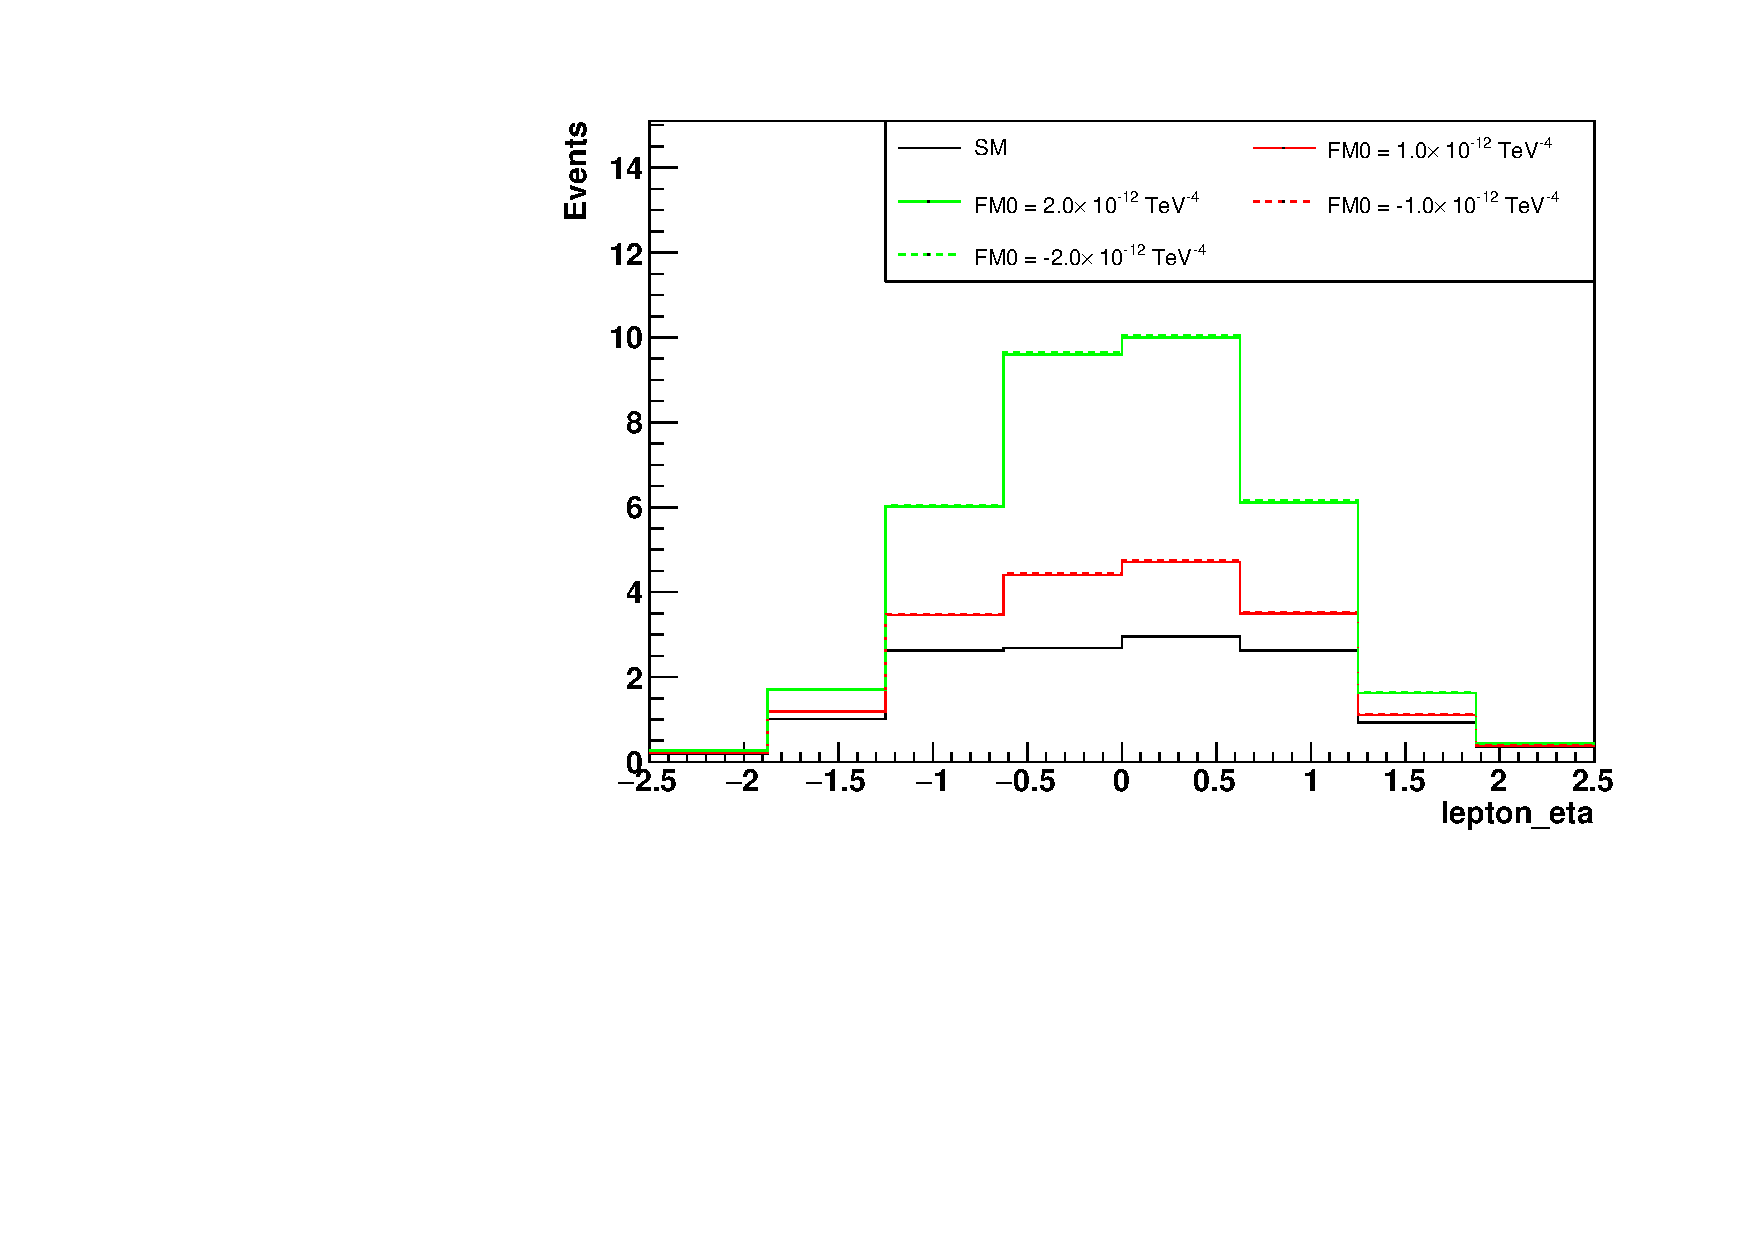
\includegraphics[width=0.45\textwidth]{Plots/aQGC_kinematics/lepton_eta_FM0.pdf}%	
	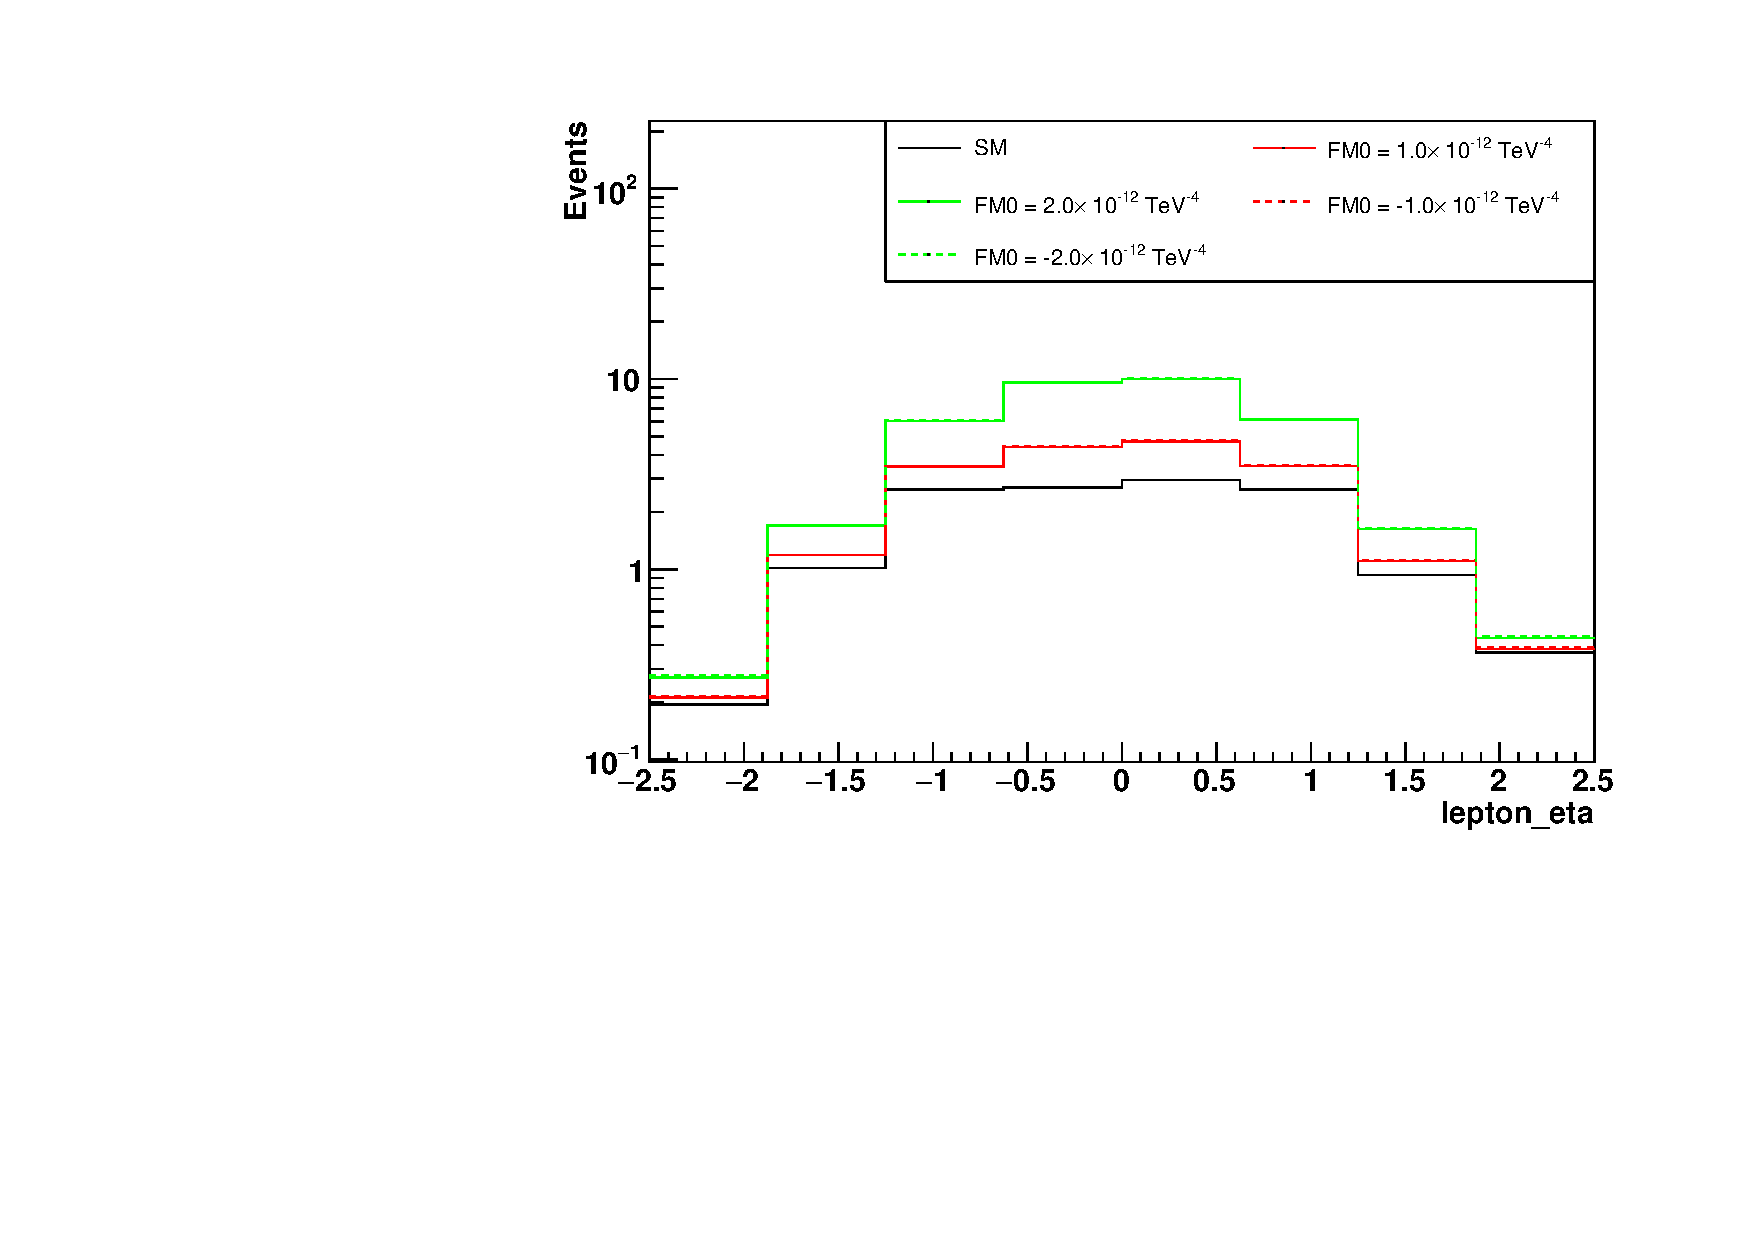
\includegraphics[width=0.45\textwidth]{Plots/aQGC_kinematics/lepton_eta_FM0_log.pdf}\\	
    \caption{}
  \end{center}
\end{figure}

\begin{figure}[h]
  \begin{center}
	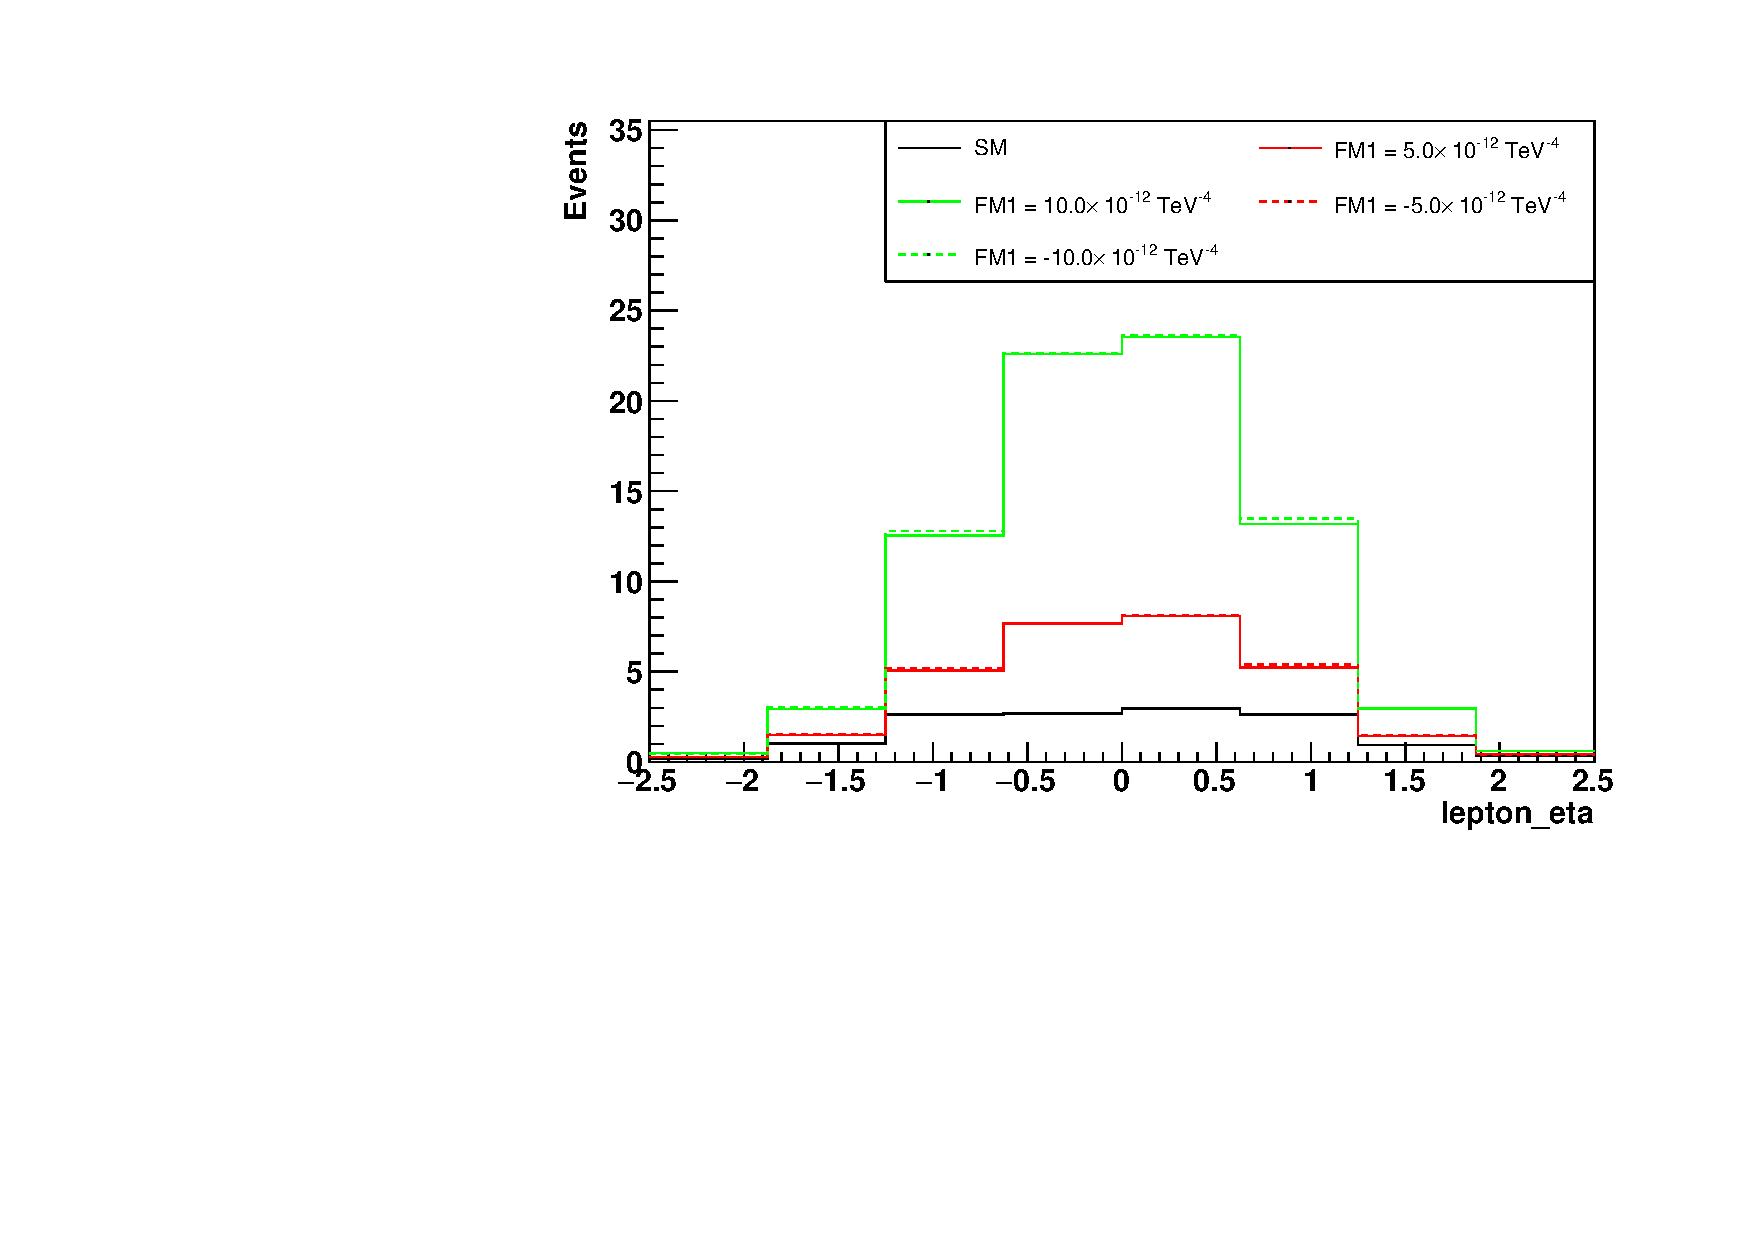
\includegraphics[width=0.45\textwidth]{Plots/aQGC_kinematics/lepton_eta_FM1.pdf}%	
	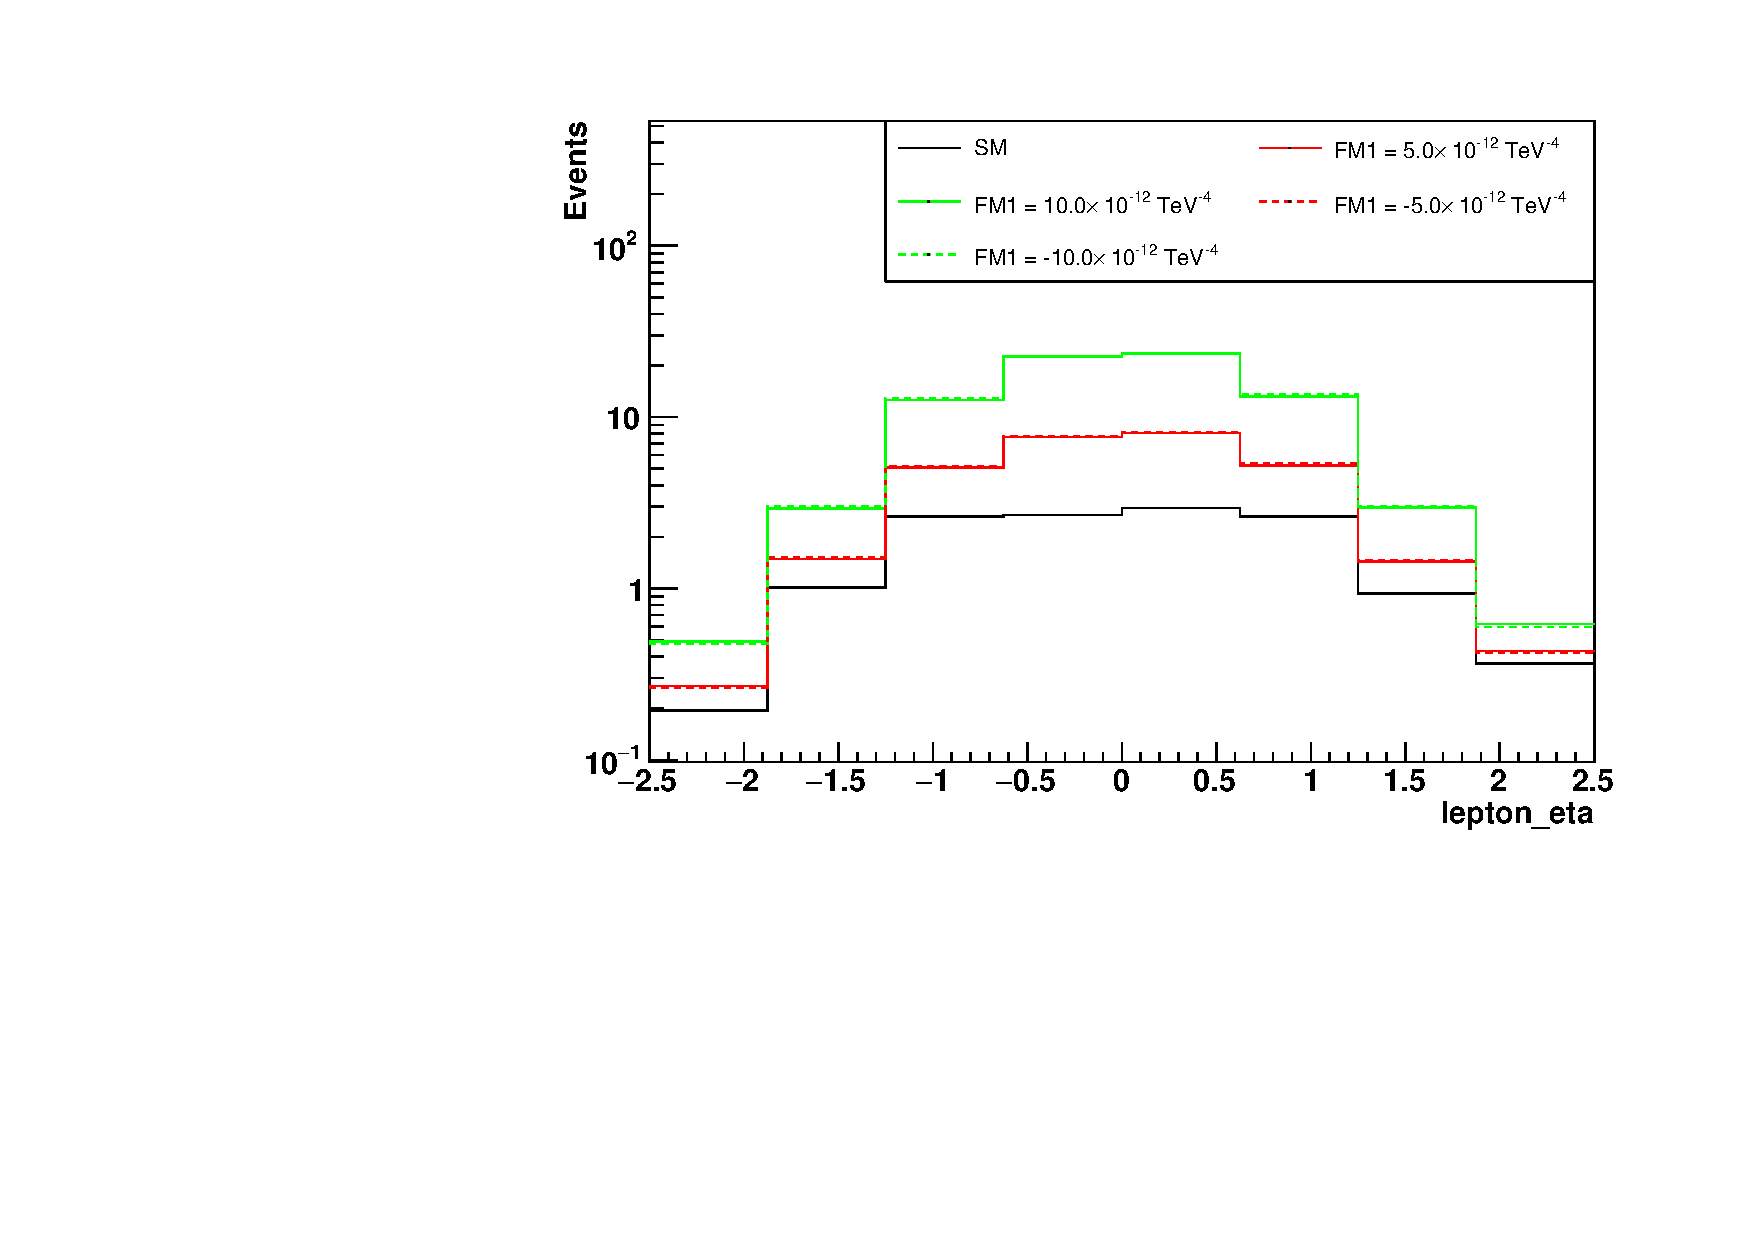
\includegraphics[width=0.45\textwidth]{Plots/aQGC_kinematics/lepton_eta_FM1_log.pdf}\\				
    \caption{}
  \end{center}
\end{figure}

\begin{figure}[h]
  \begin{center}
	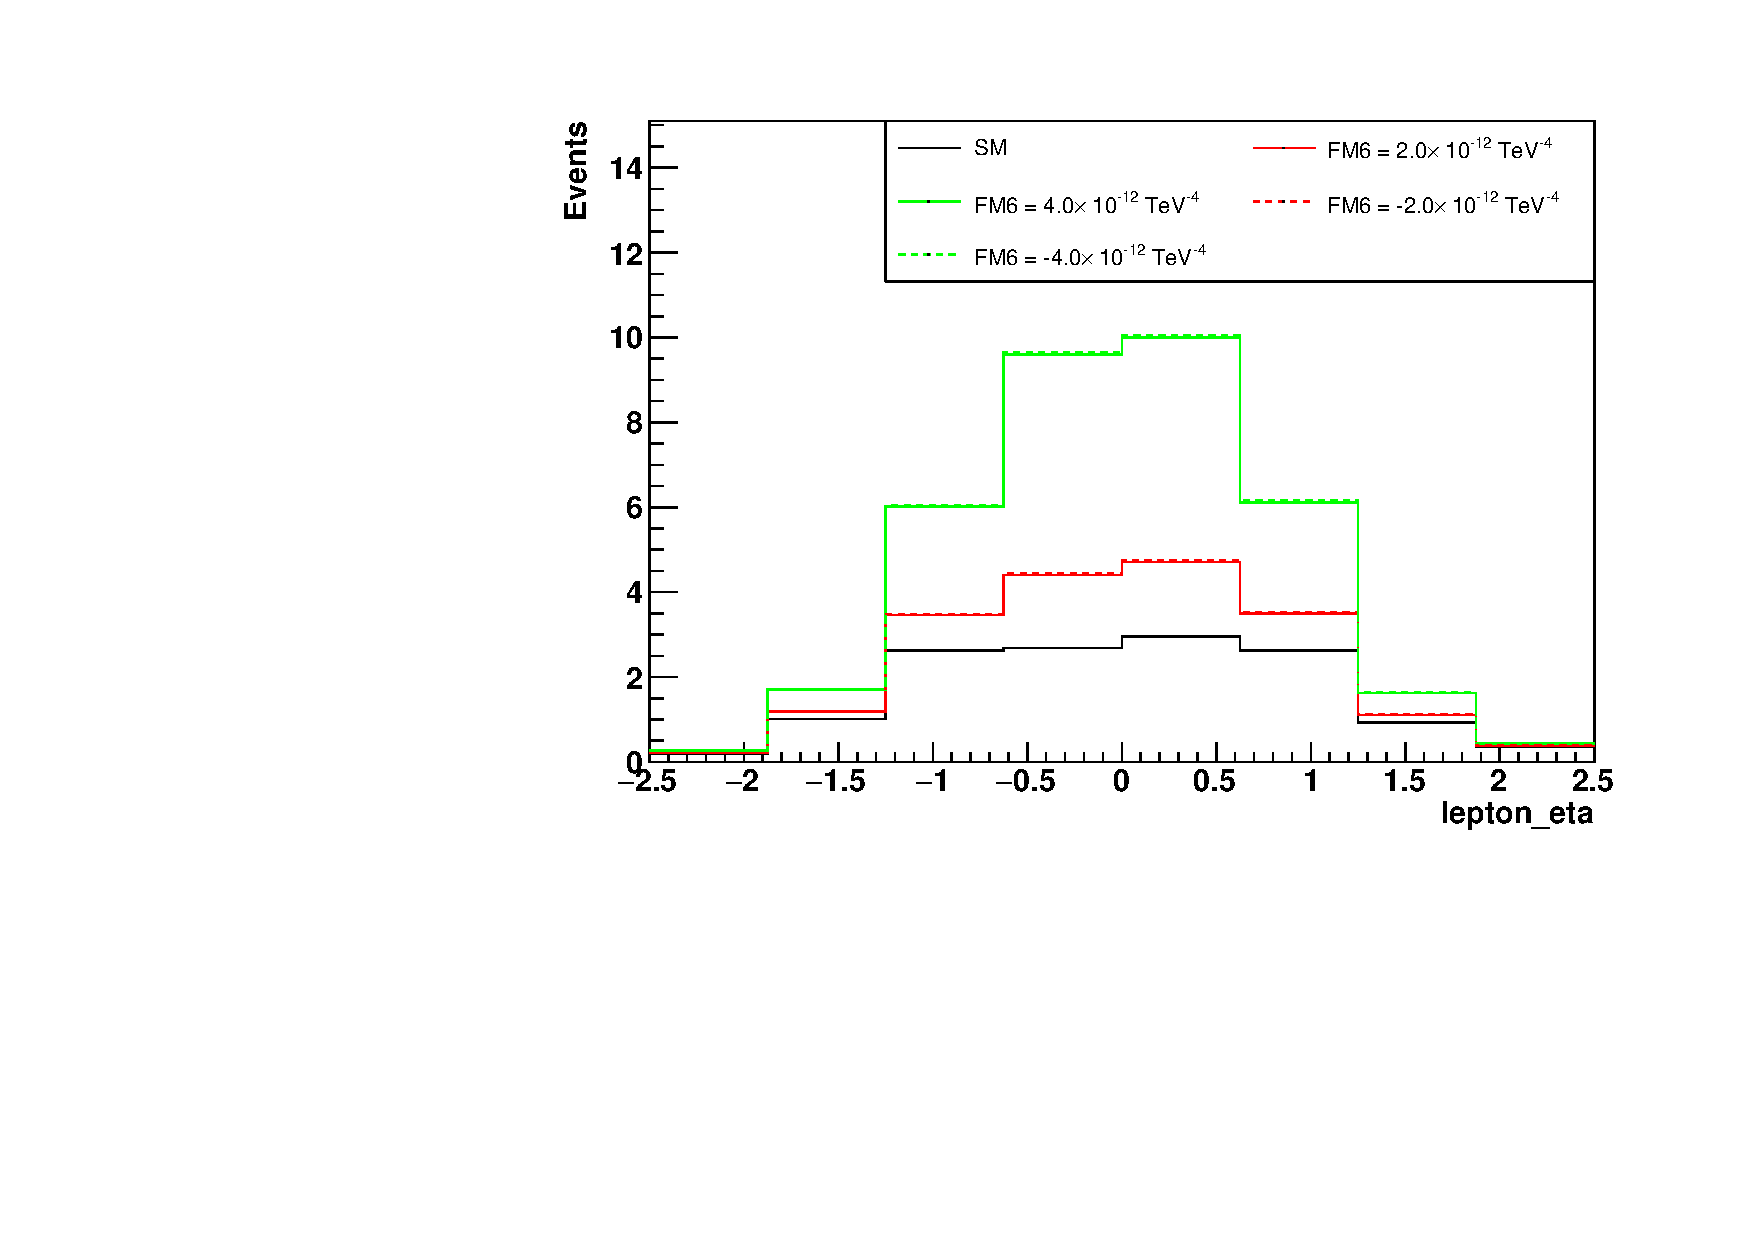
\includegraphics[width=0.45\textwidth]{Plots/aQGC_kinematics/lepton_eta_FM6.pdf}%	
	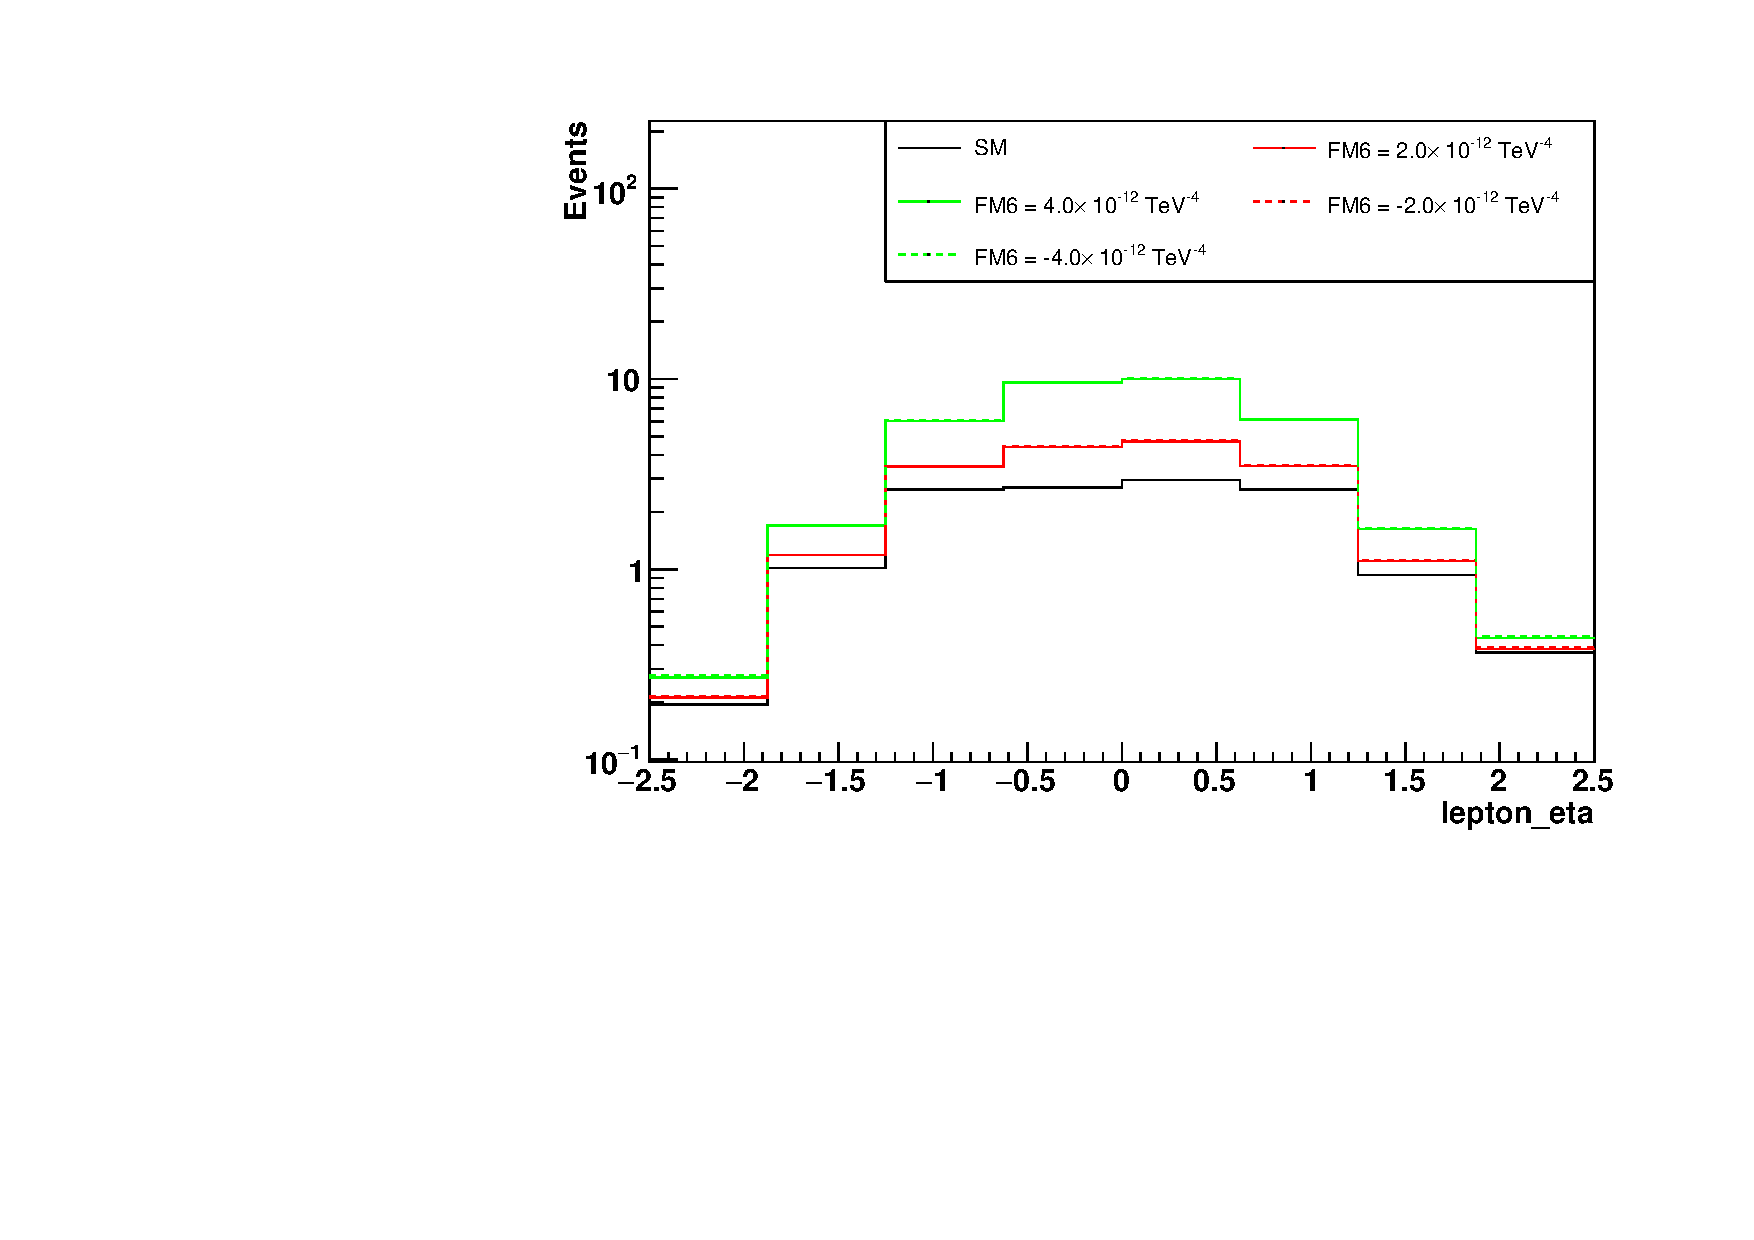
\includegraphics[width=0.45\textwidth]{Plots/aQGC_kinematics/lepton_eta_FM6_log.pdf}\\				
    \caption{}
  \end{center}
\end{figure}

\begin{figure}[h]
  \begin{center}
	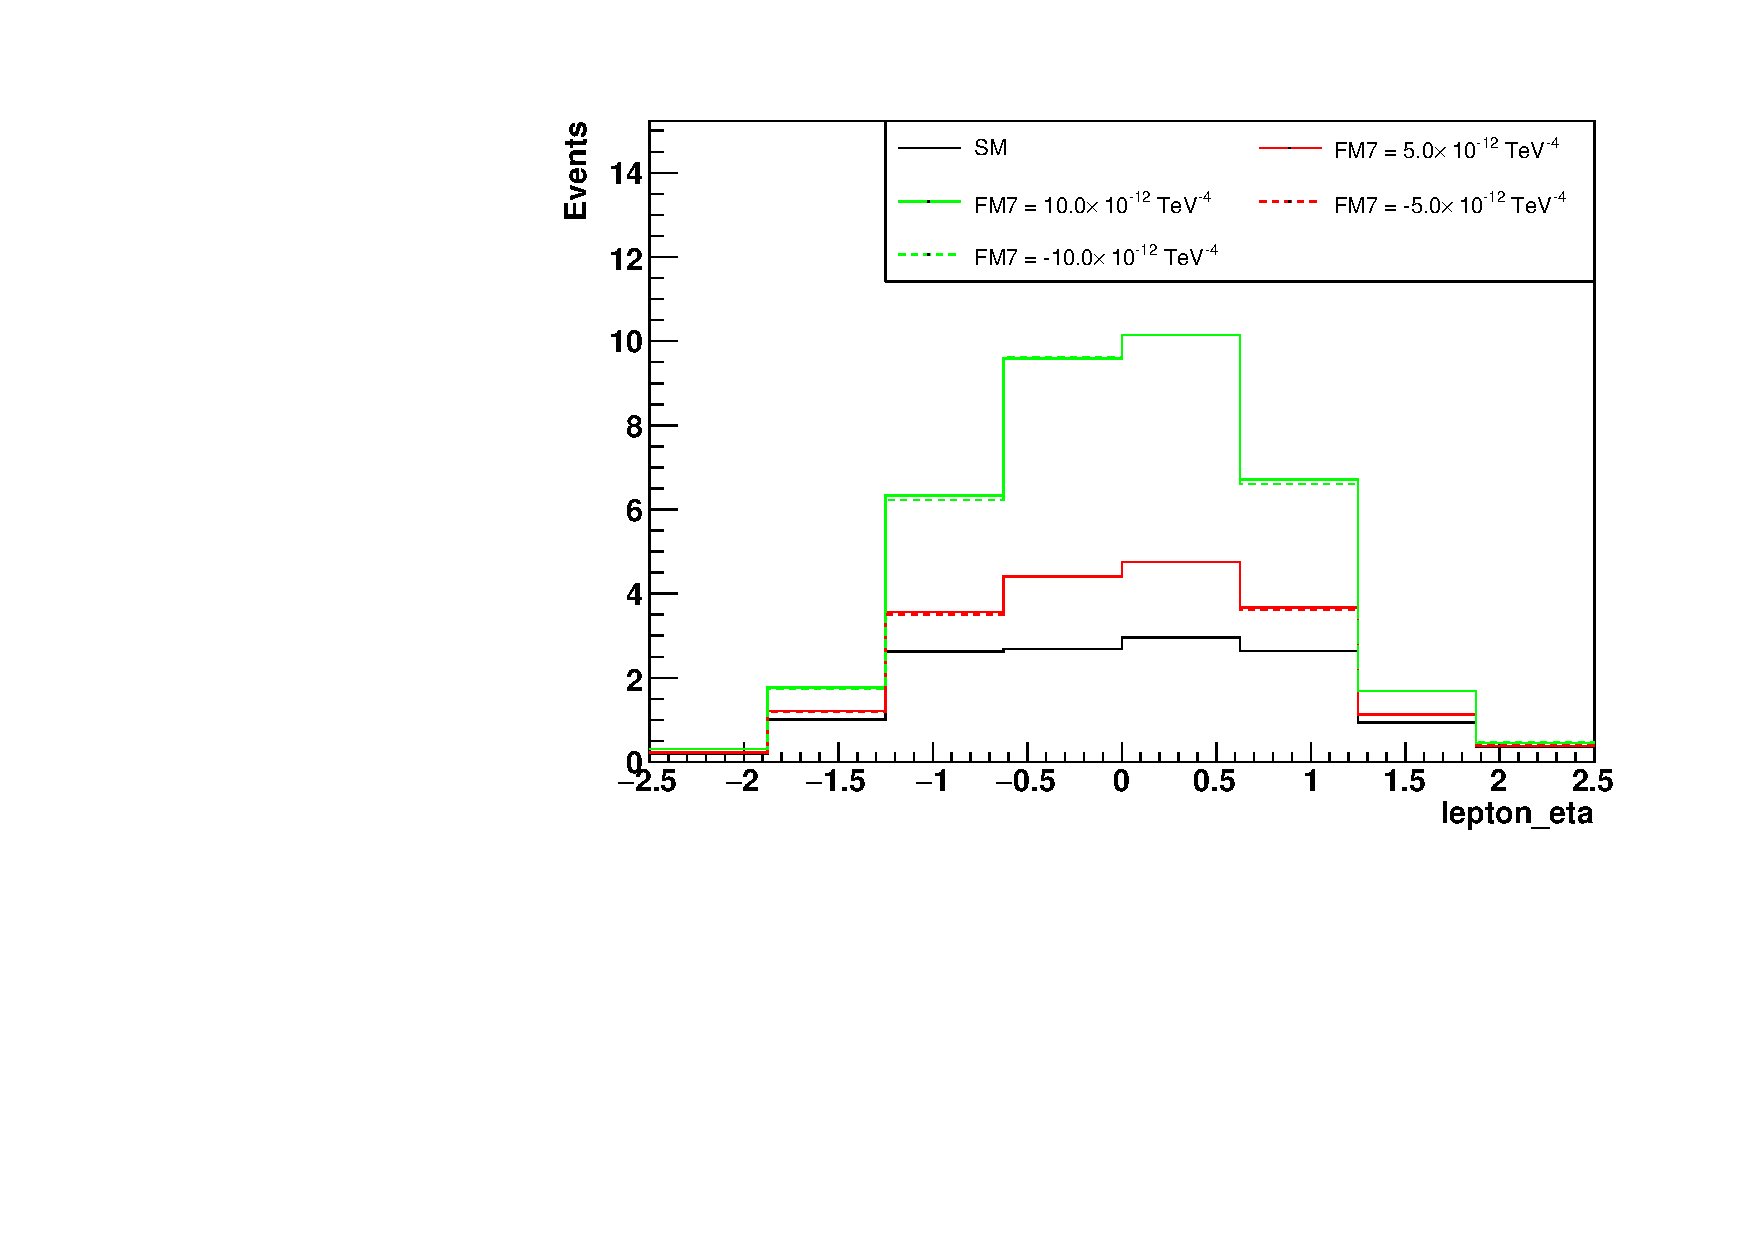
\includegraphics[width=0.45\textwidth]{Plots/aQGC_kinematics/lepton_eta_FM7.pdf}%	
	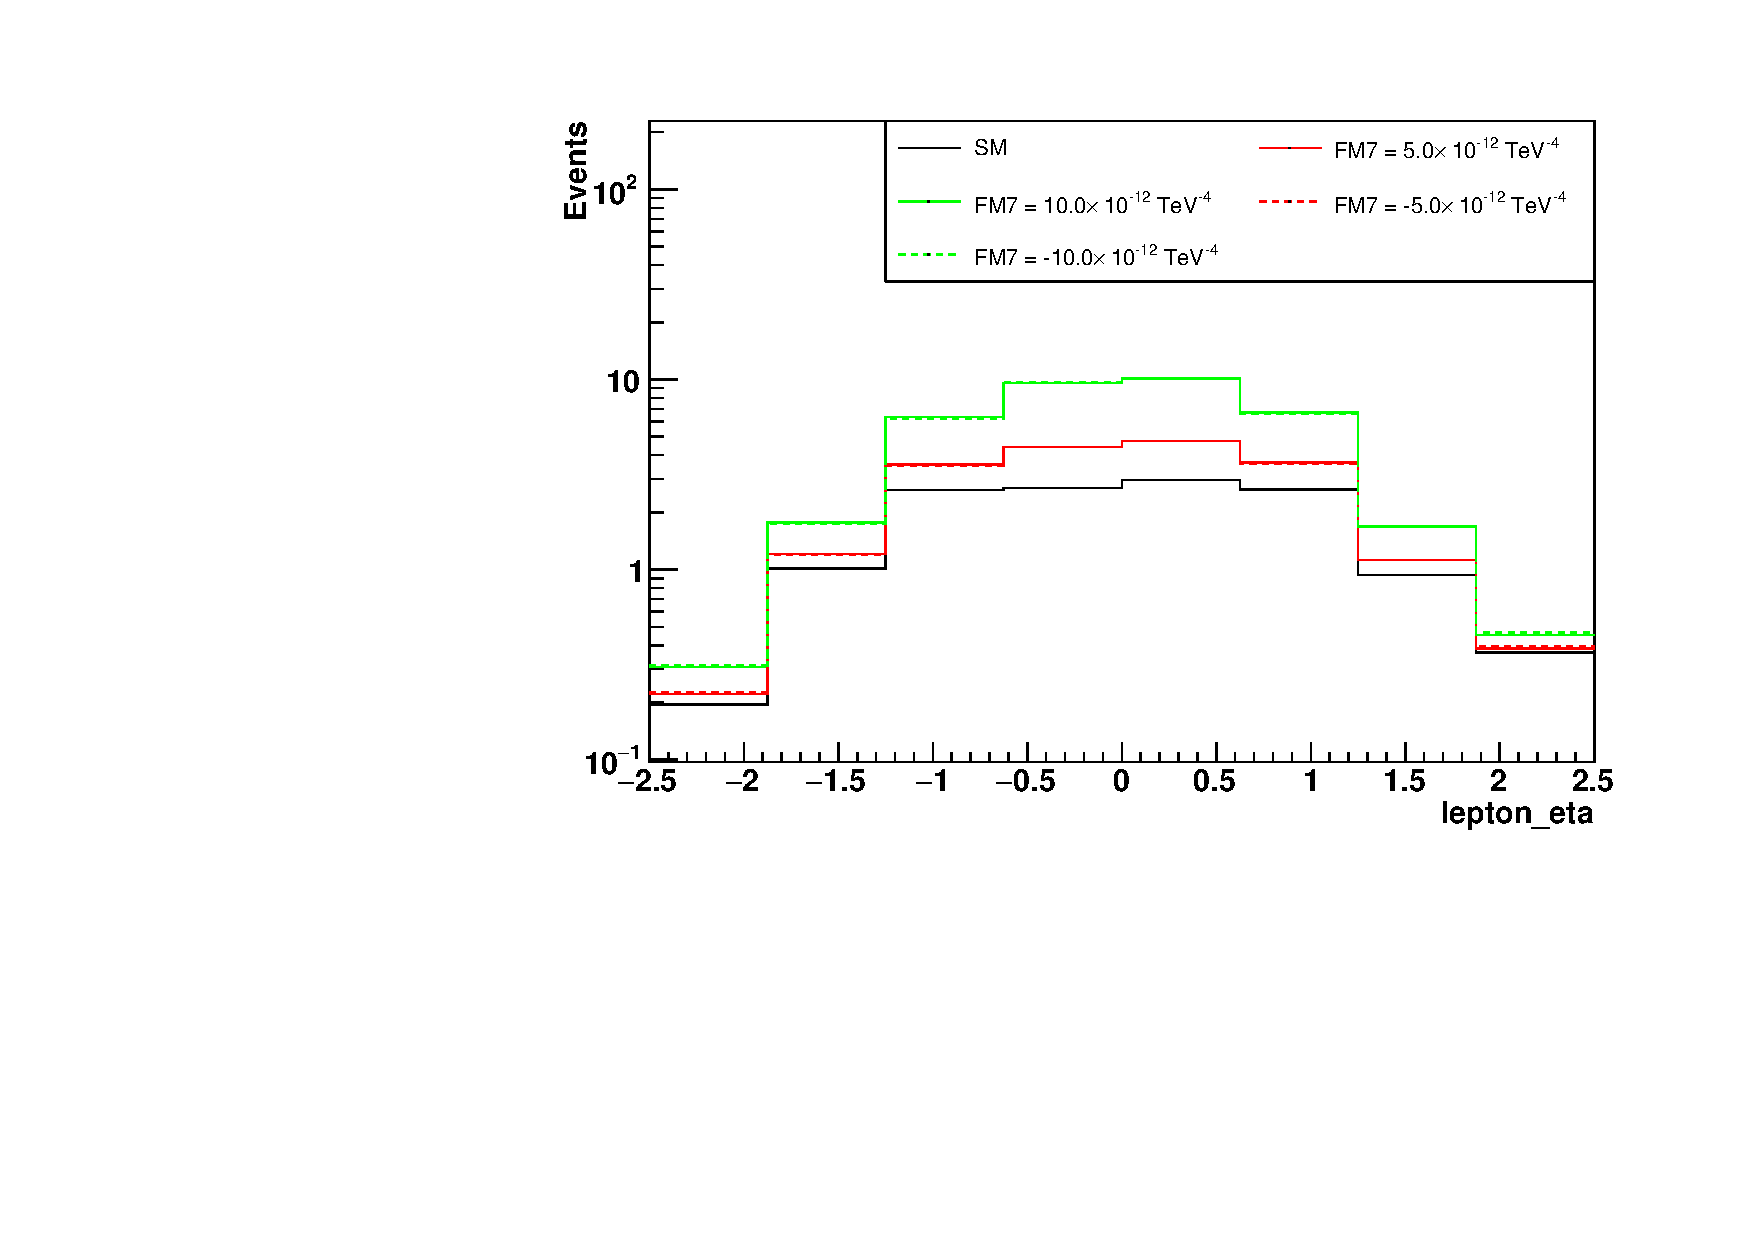
\includegraphics[width=0.45\textwidth]{Plots/aQGC_kinematics/lepton_eta_FM7_log.pdf}\\				
    \caption{}
  \end{center}
\end{figure}

\begin{figure}[h]
  \begin{center}
	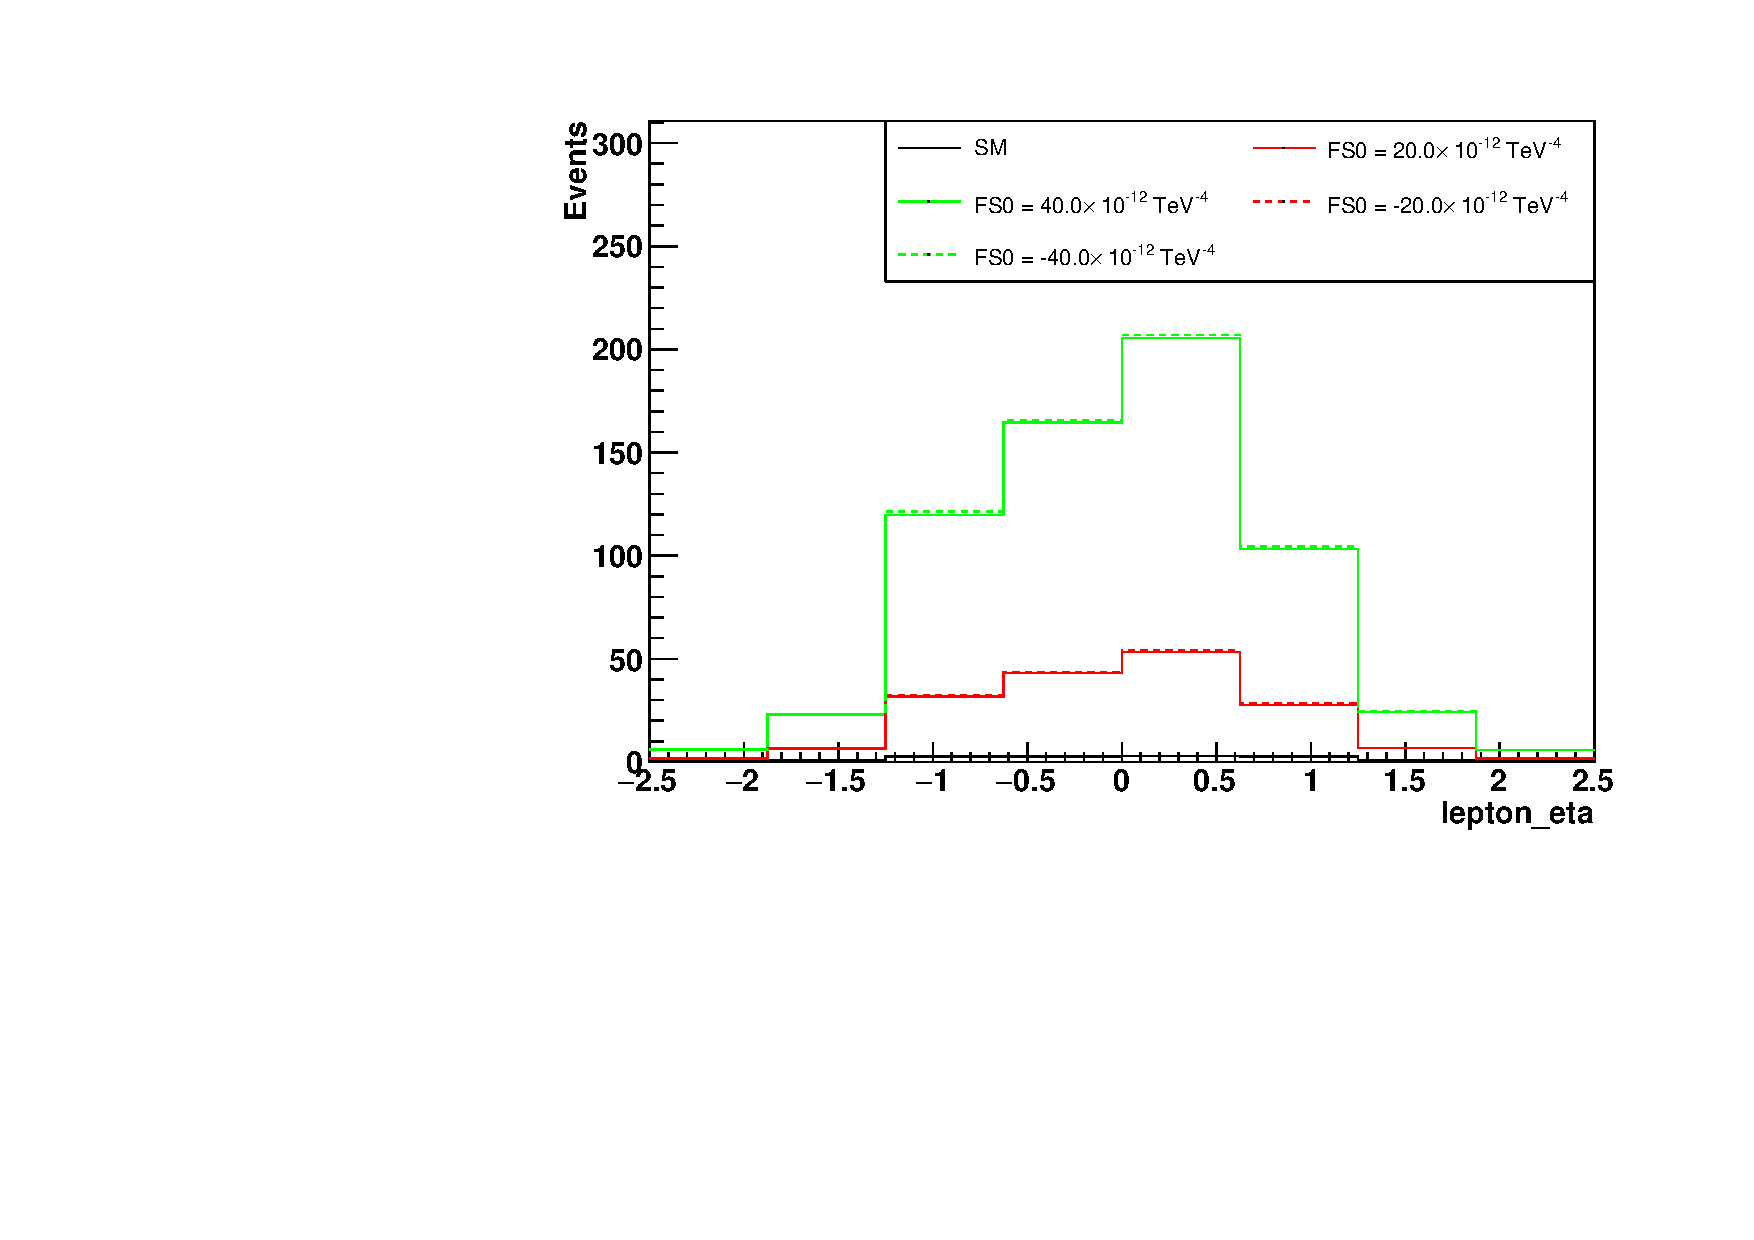
\includegraphics[width=0.45\textwidth]{Plots/aQGC_kinematics/lepton_eta_FS0.pdf}%	
	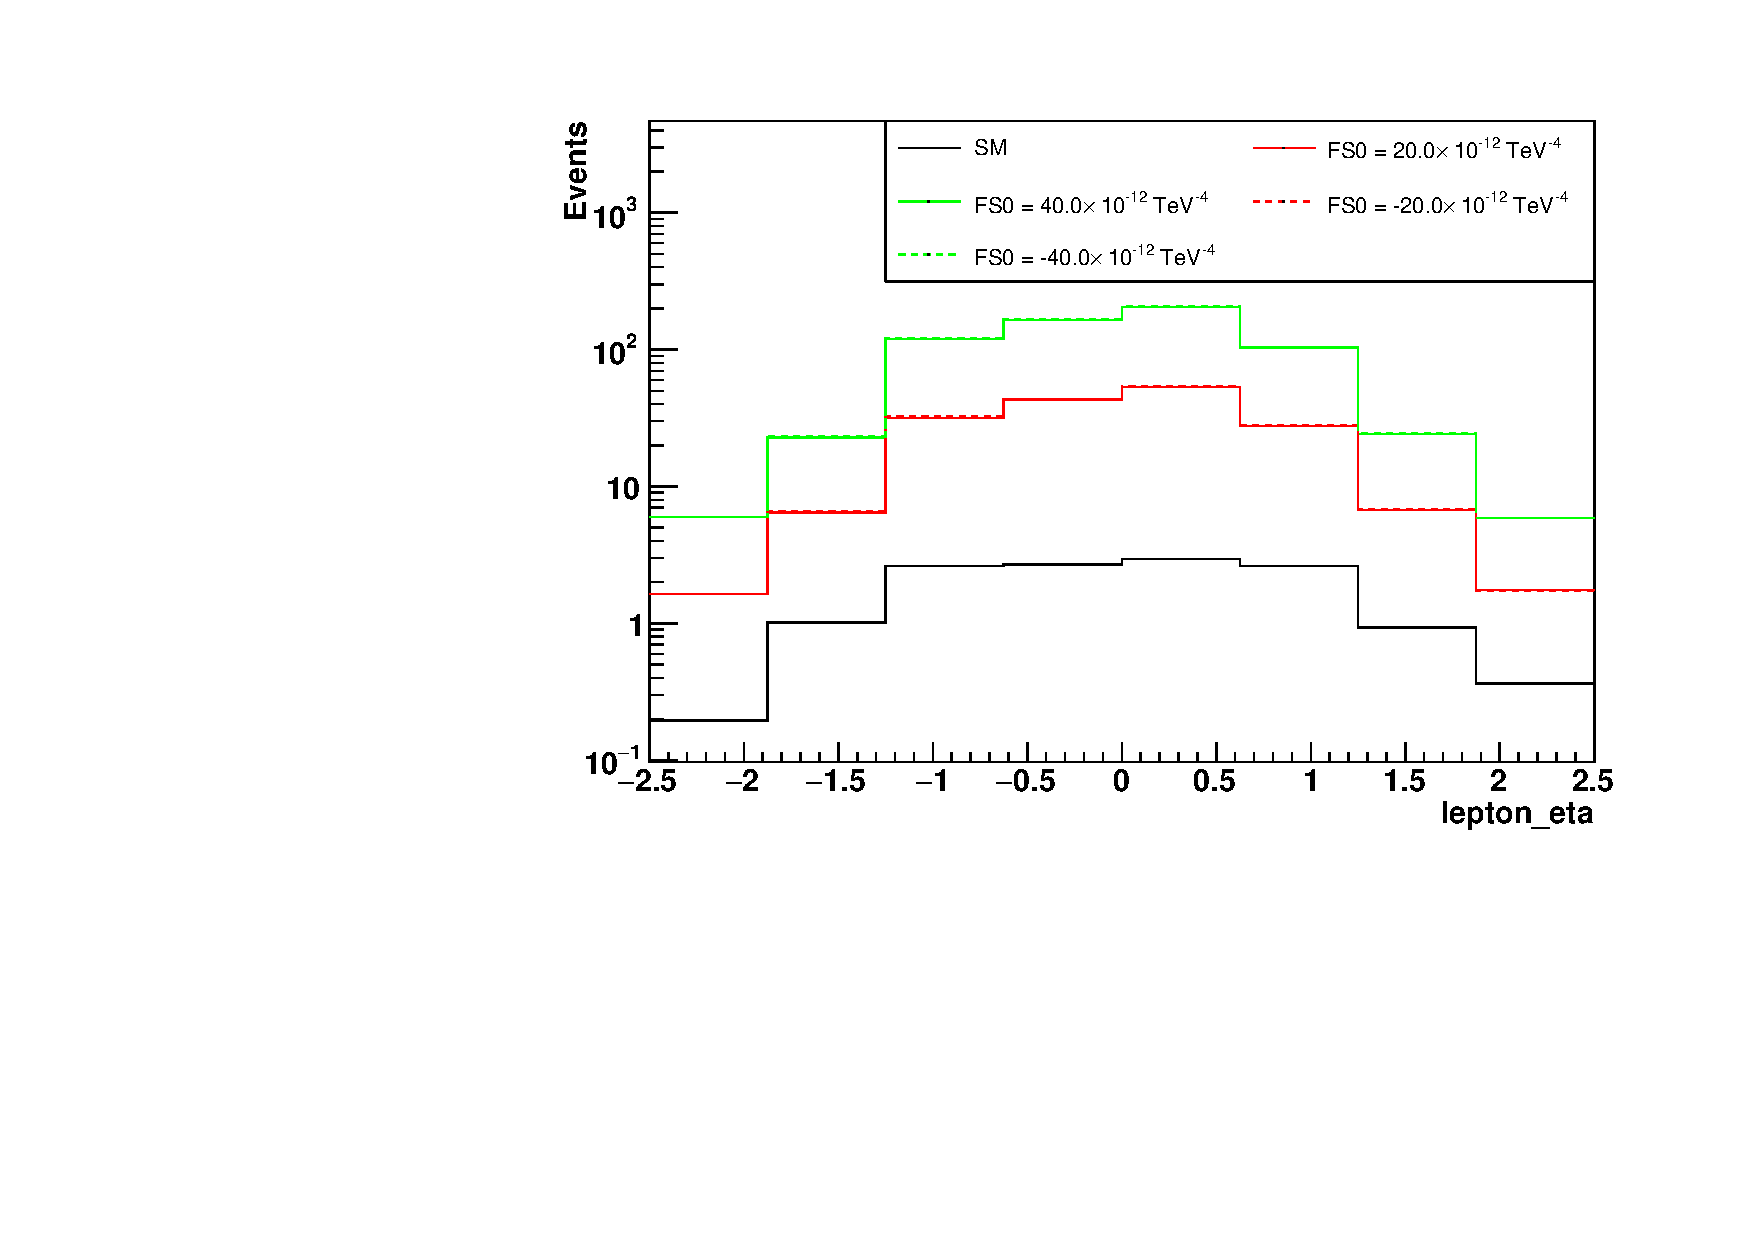
\includegraphics[width=0.45\textwidth]{Plots/aQGC_kinematics/lepton_eta_FS0_log.pdf}\\				
    \caption{}
  \end{center}
\end{figure}

\begin{figure}[h]
  \begin{center}
	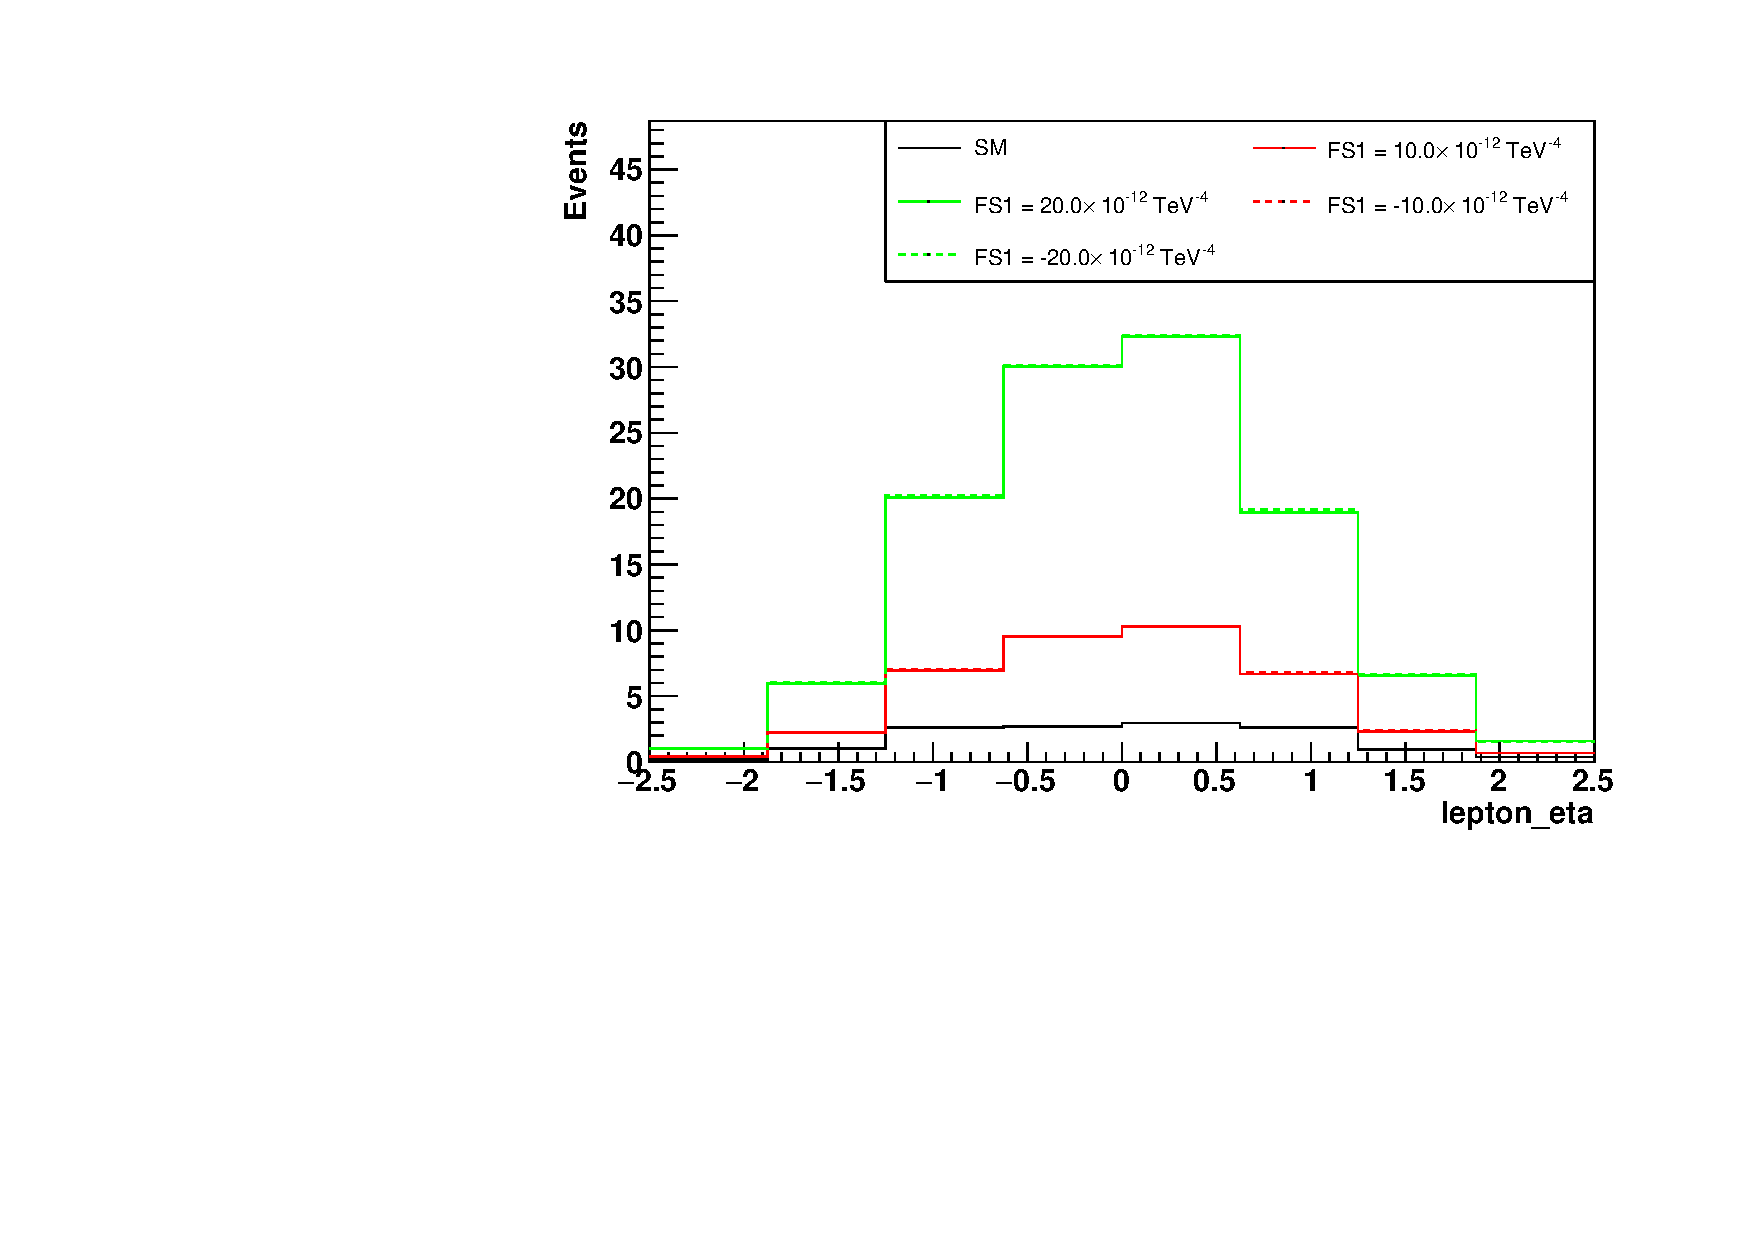
\includegraphics[width=0.45\textwidth]{Plots/aQGC_kinematics/lepton_eta_FS1.pdf}%	
	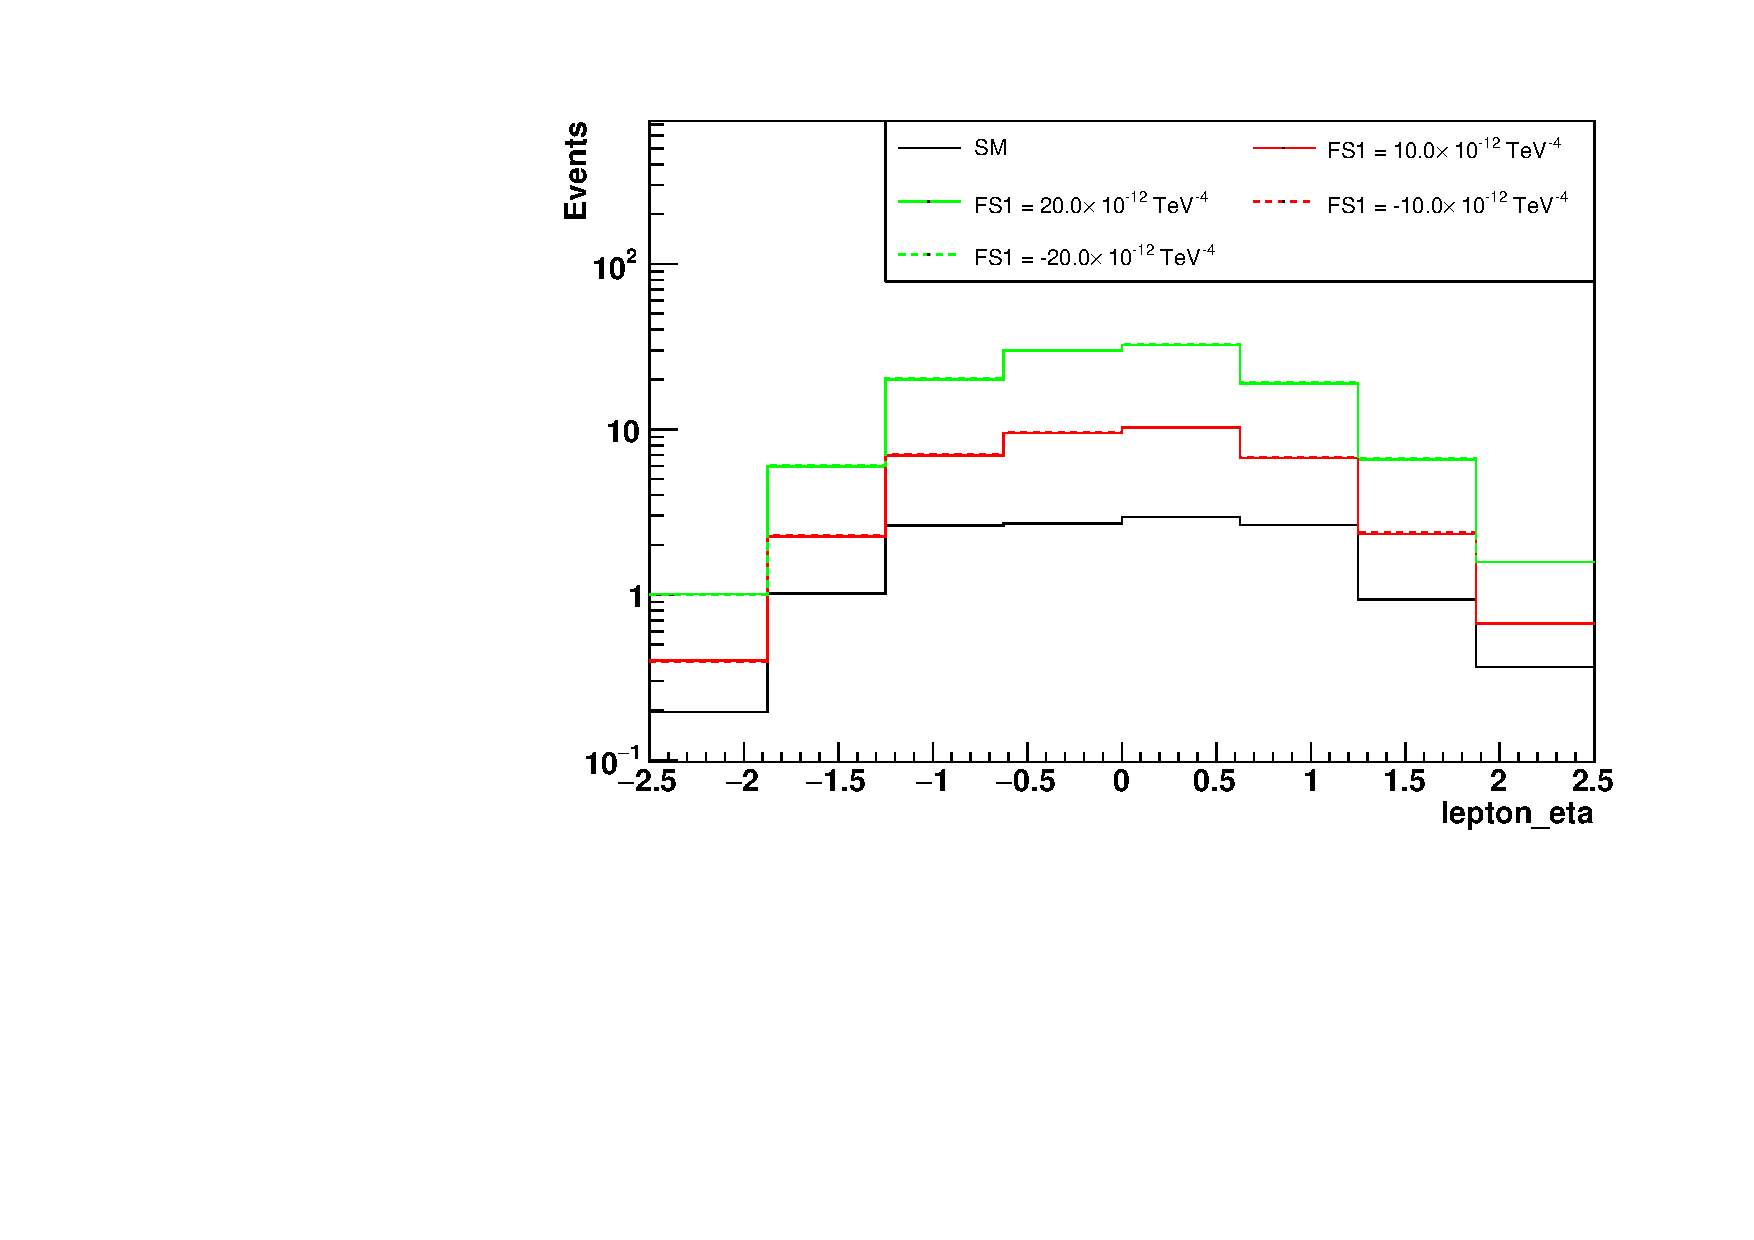
\includegraphics[width=0.45\textwidth]{Plots/aQGC_kinematics/lepton_eta_FS1_log.pdf}\\				
    \caption{}
  \end{center}
\end{figure}

\begin{figure}[h]
  \begin{center}
	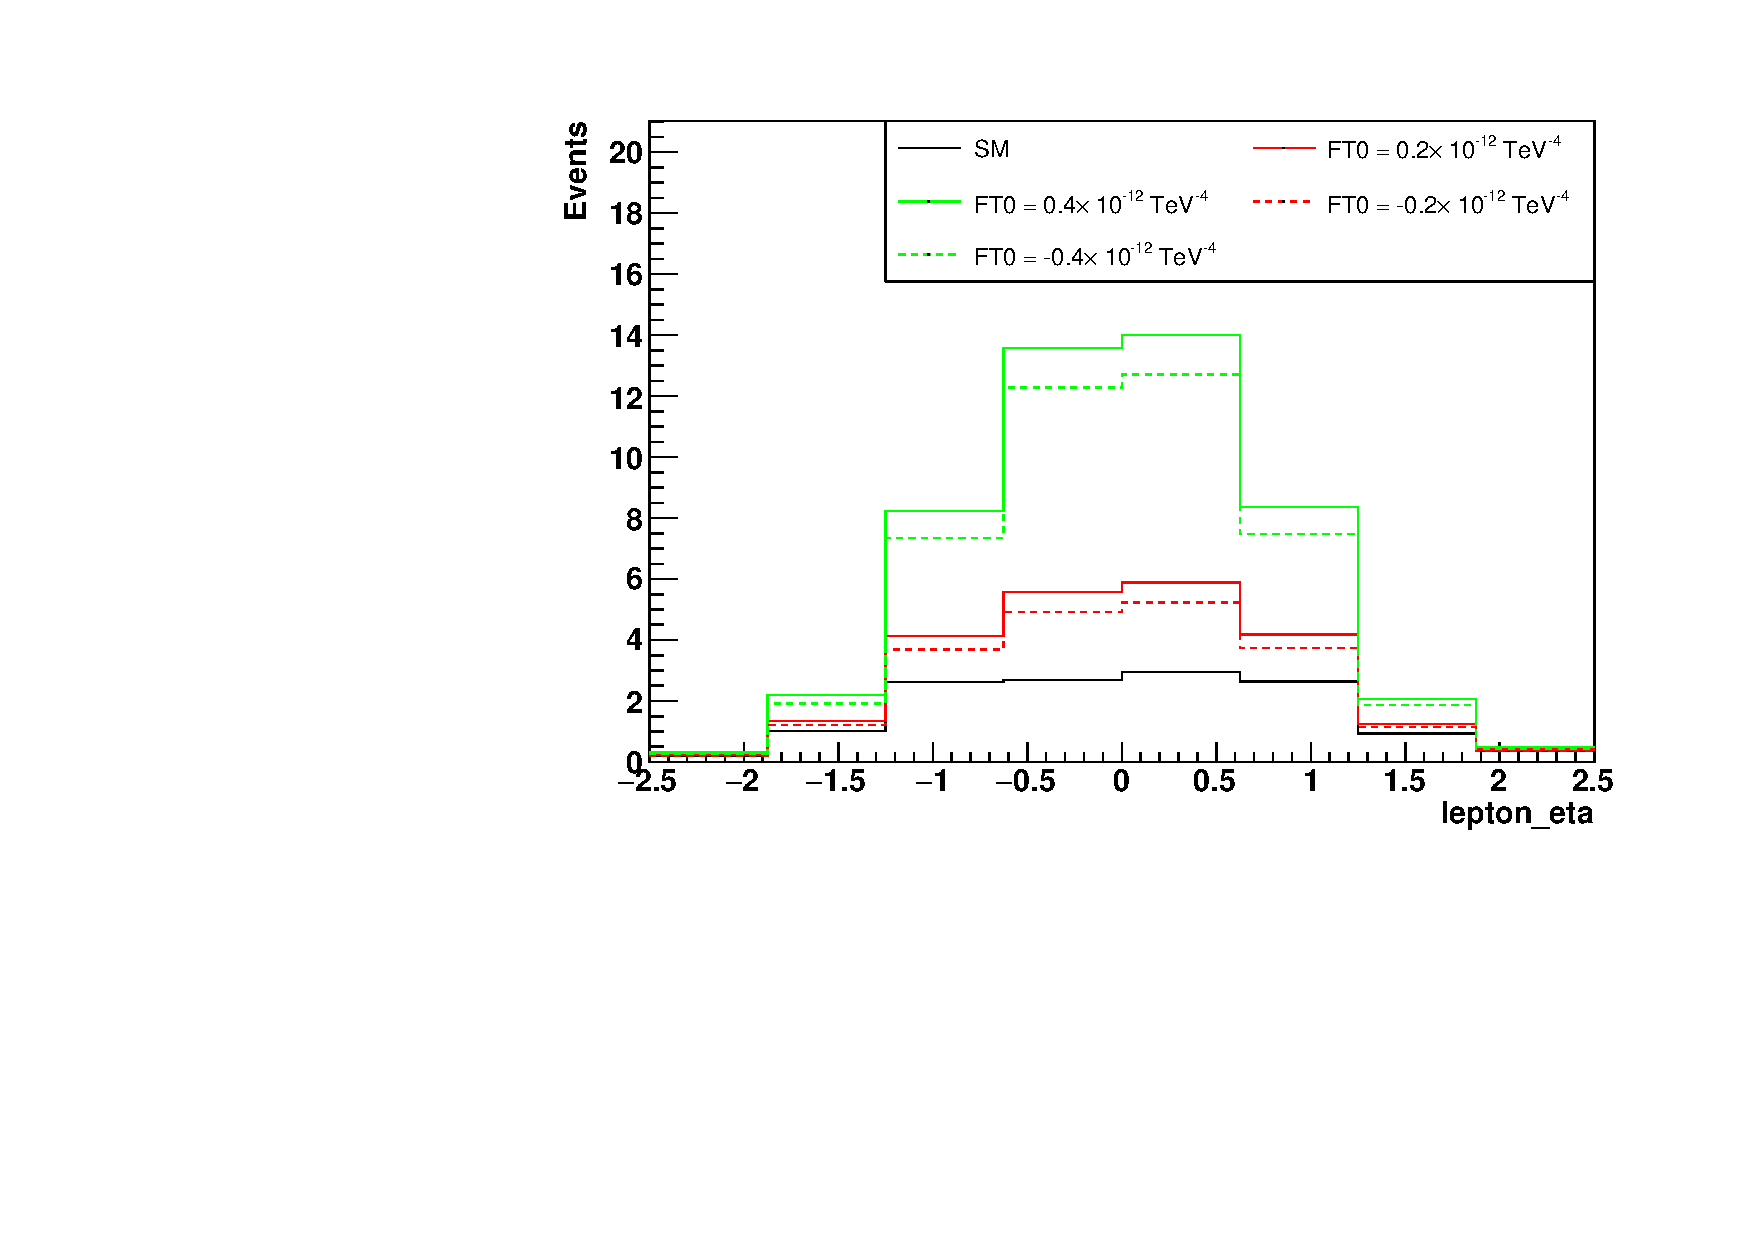
\includegraphics[width=0.45\textwidth]{Plots/aQGC_kinematics/lepton_eta_FT0.pdf}%	
	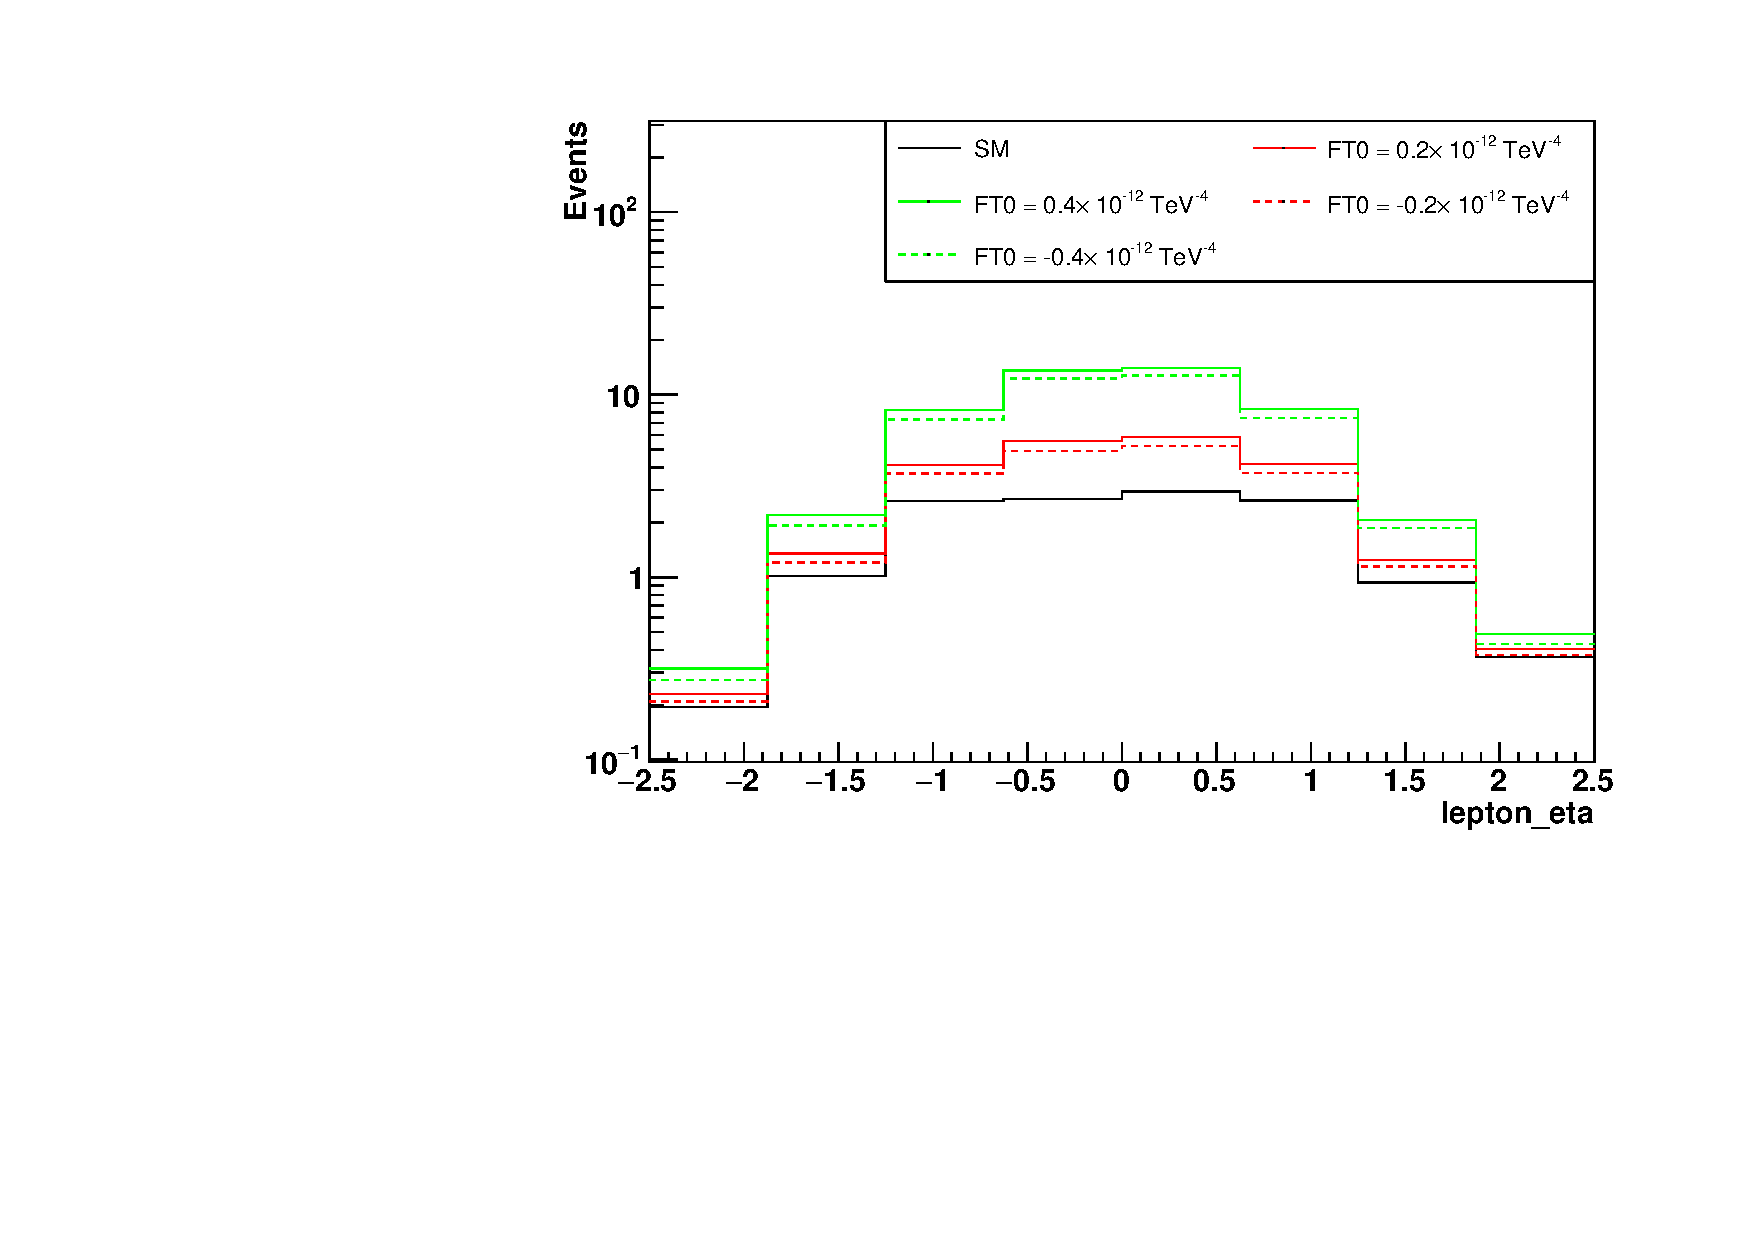
\includegraphics[width=0.45\textwidth]{Plots/aQGC_kinematics/lepton_eta_FT0_log.pdf}\\				
    \caption{}
  \end{center}
\end{figure}

\begin{figure}[h]
  \begin{center}
	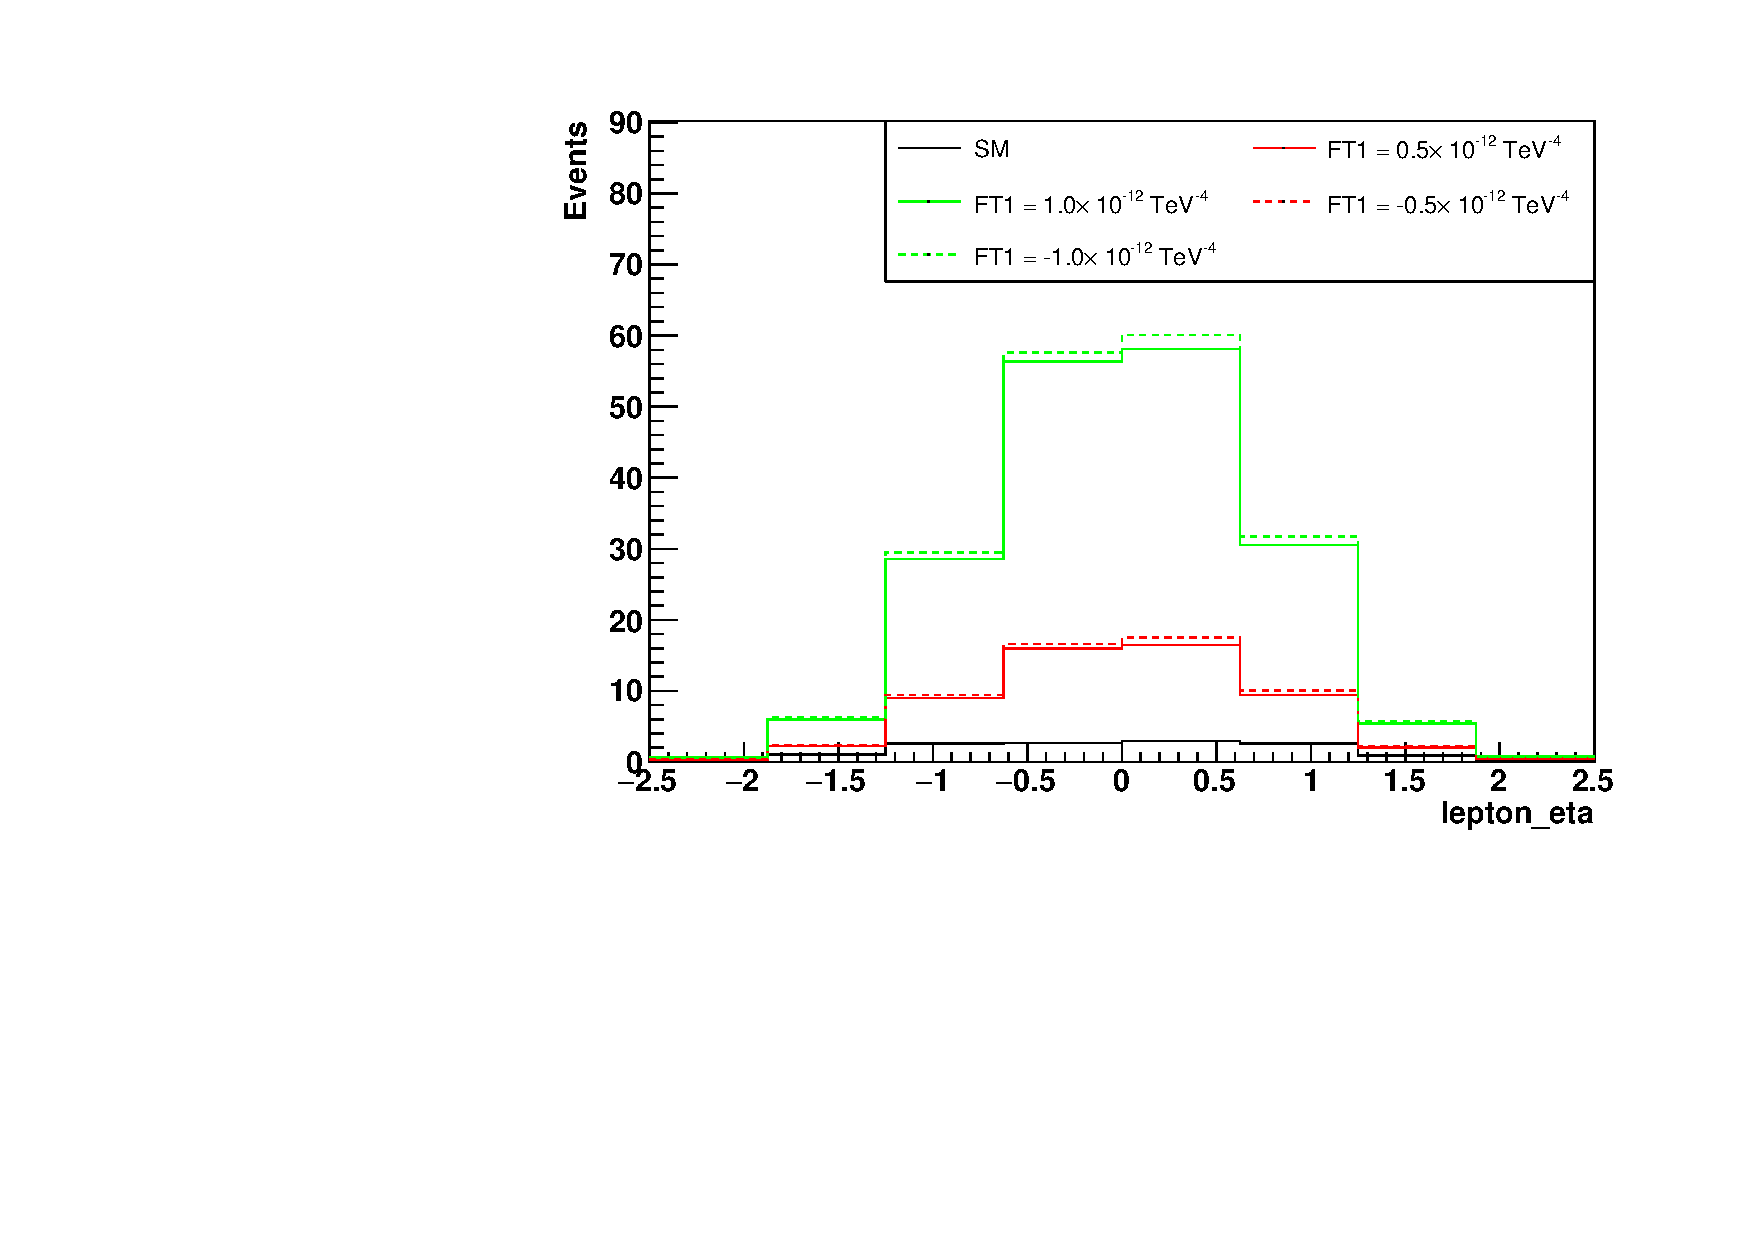
\includegraphics[width=0.45\textwidth]{Plots/aQGC_kinematics/lepton_eta_FT1.pdf}%	
	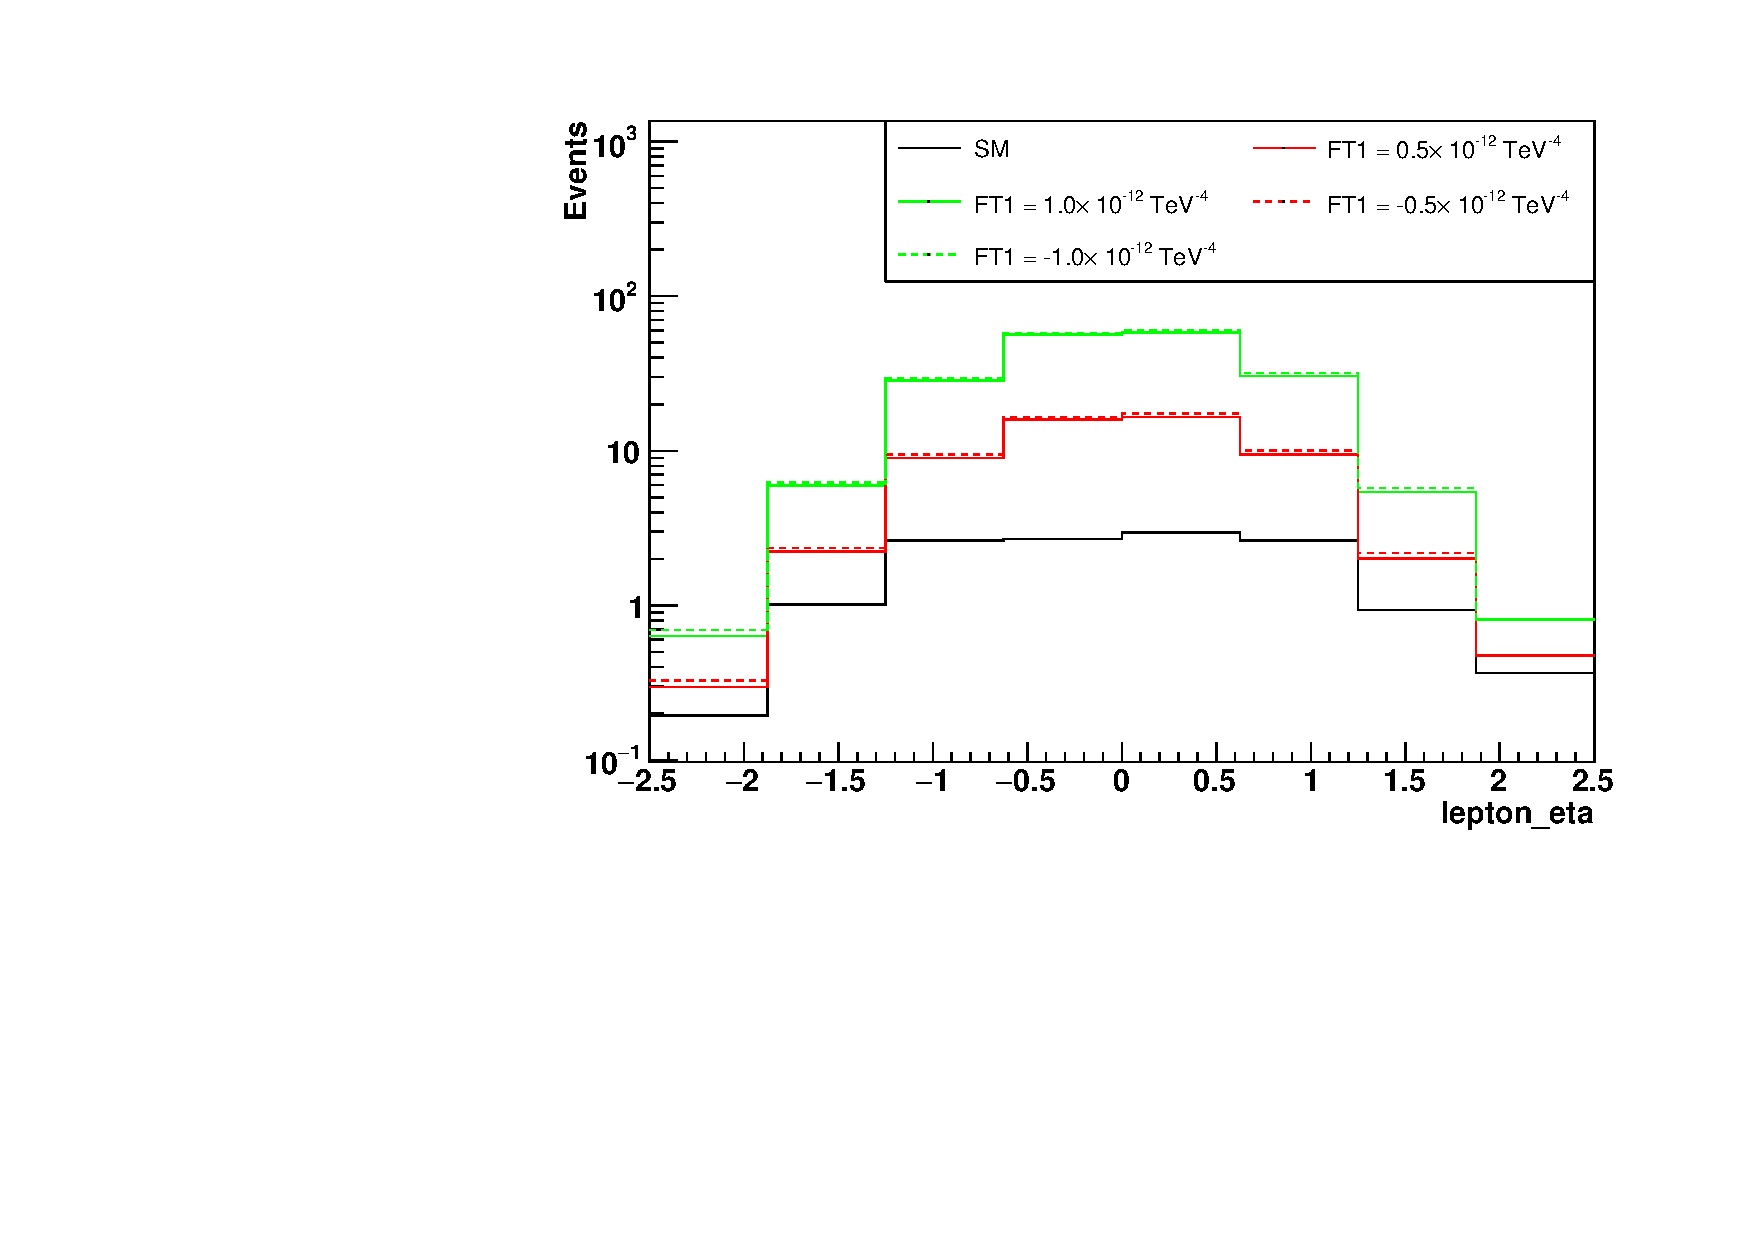
\includegraphics[width=0.45\textwidth]{Plots/aQGC_kinematics/lepton_eta_FT1_log.pdf}\\				
    \caption{}
  \end{center}
\end{figure}

\begin{figure}[h]
  \begin{center}
	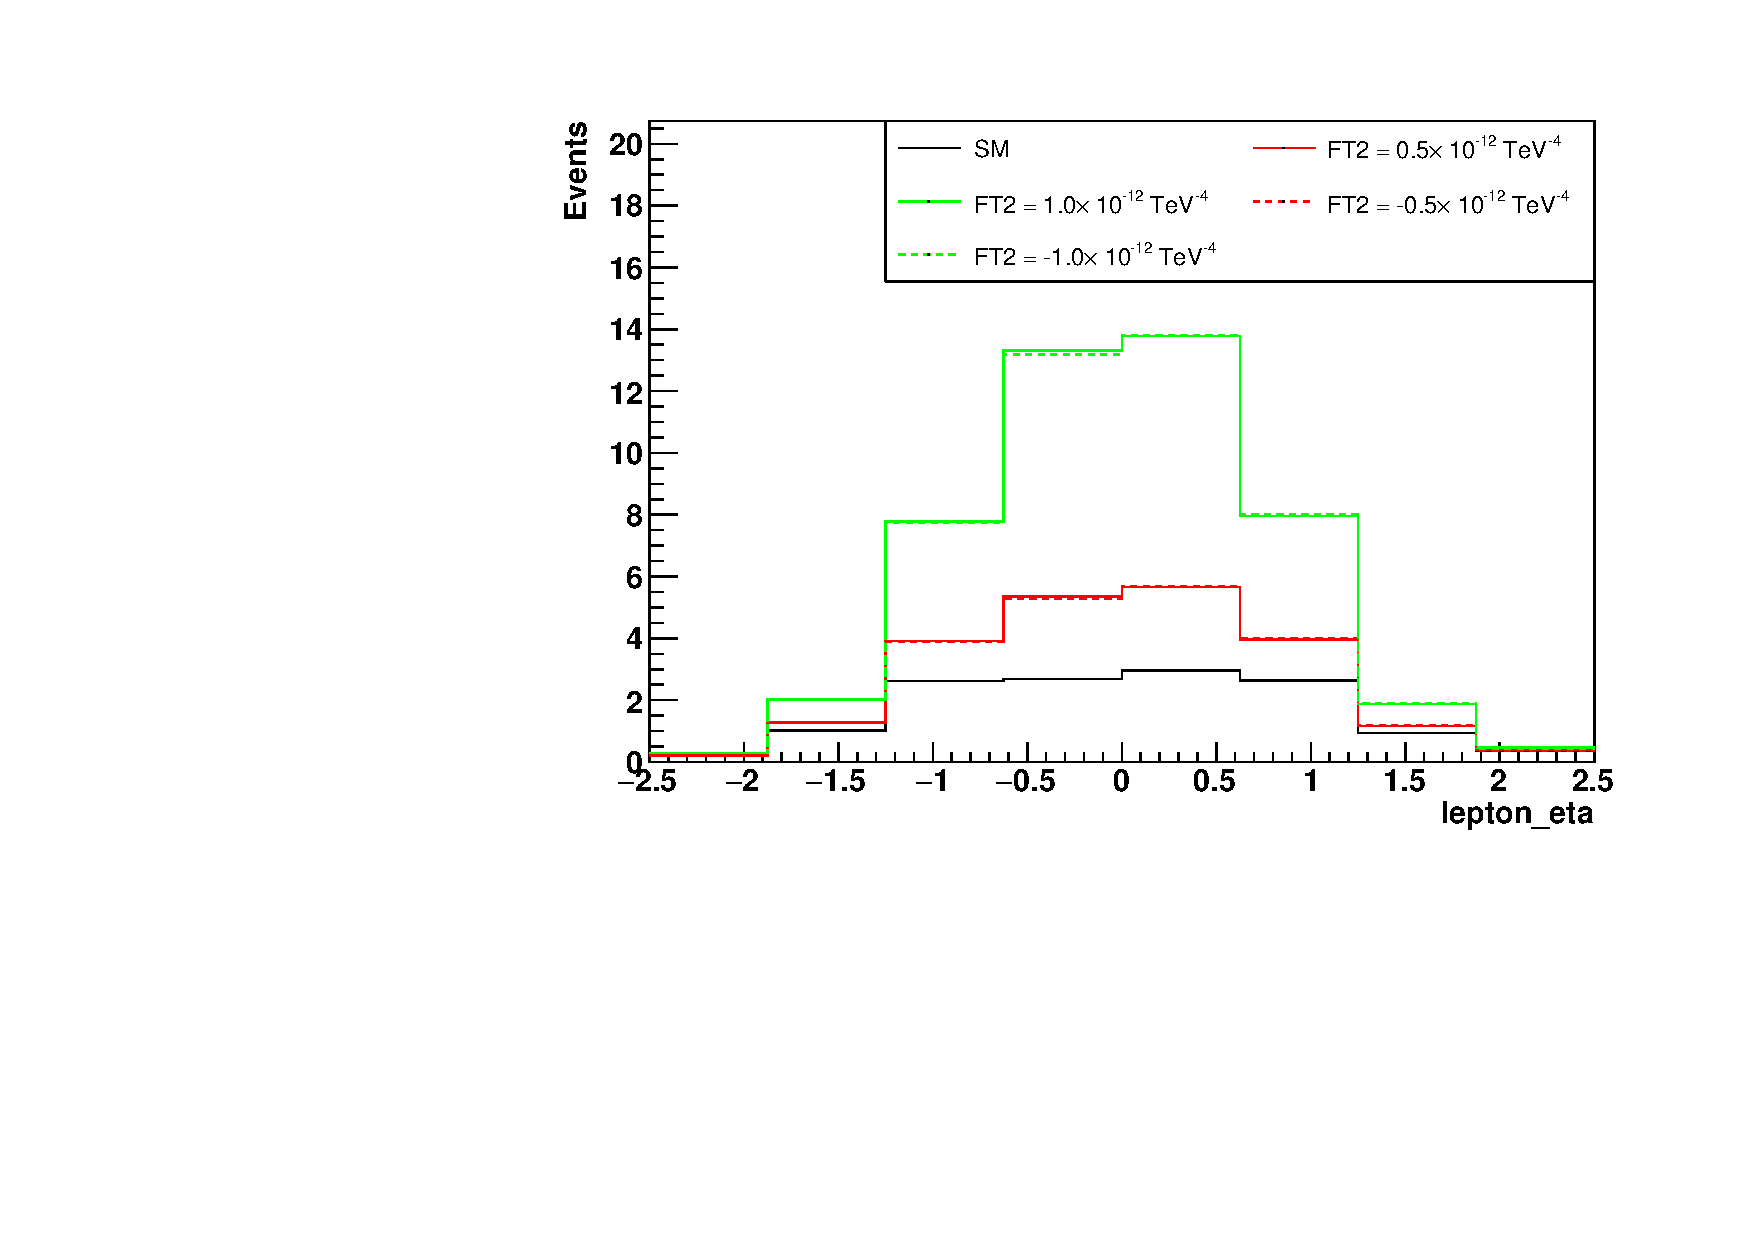
\includegraphics[width=0.45\textwidth]{Plots/aQGC_kinematics/lepton_eta_FT2.pdf}%	
	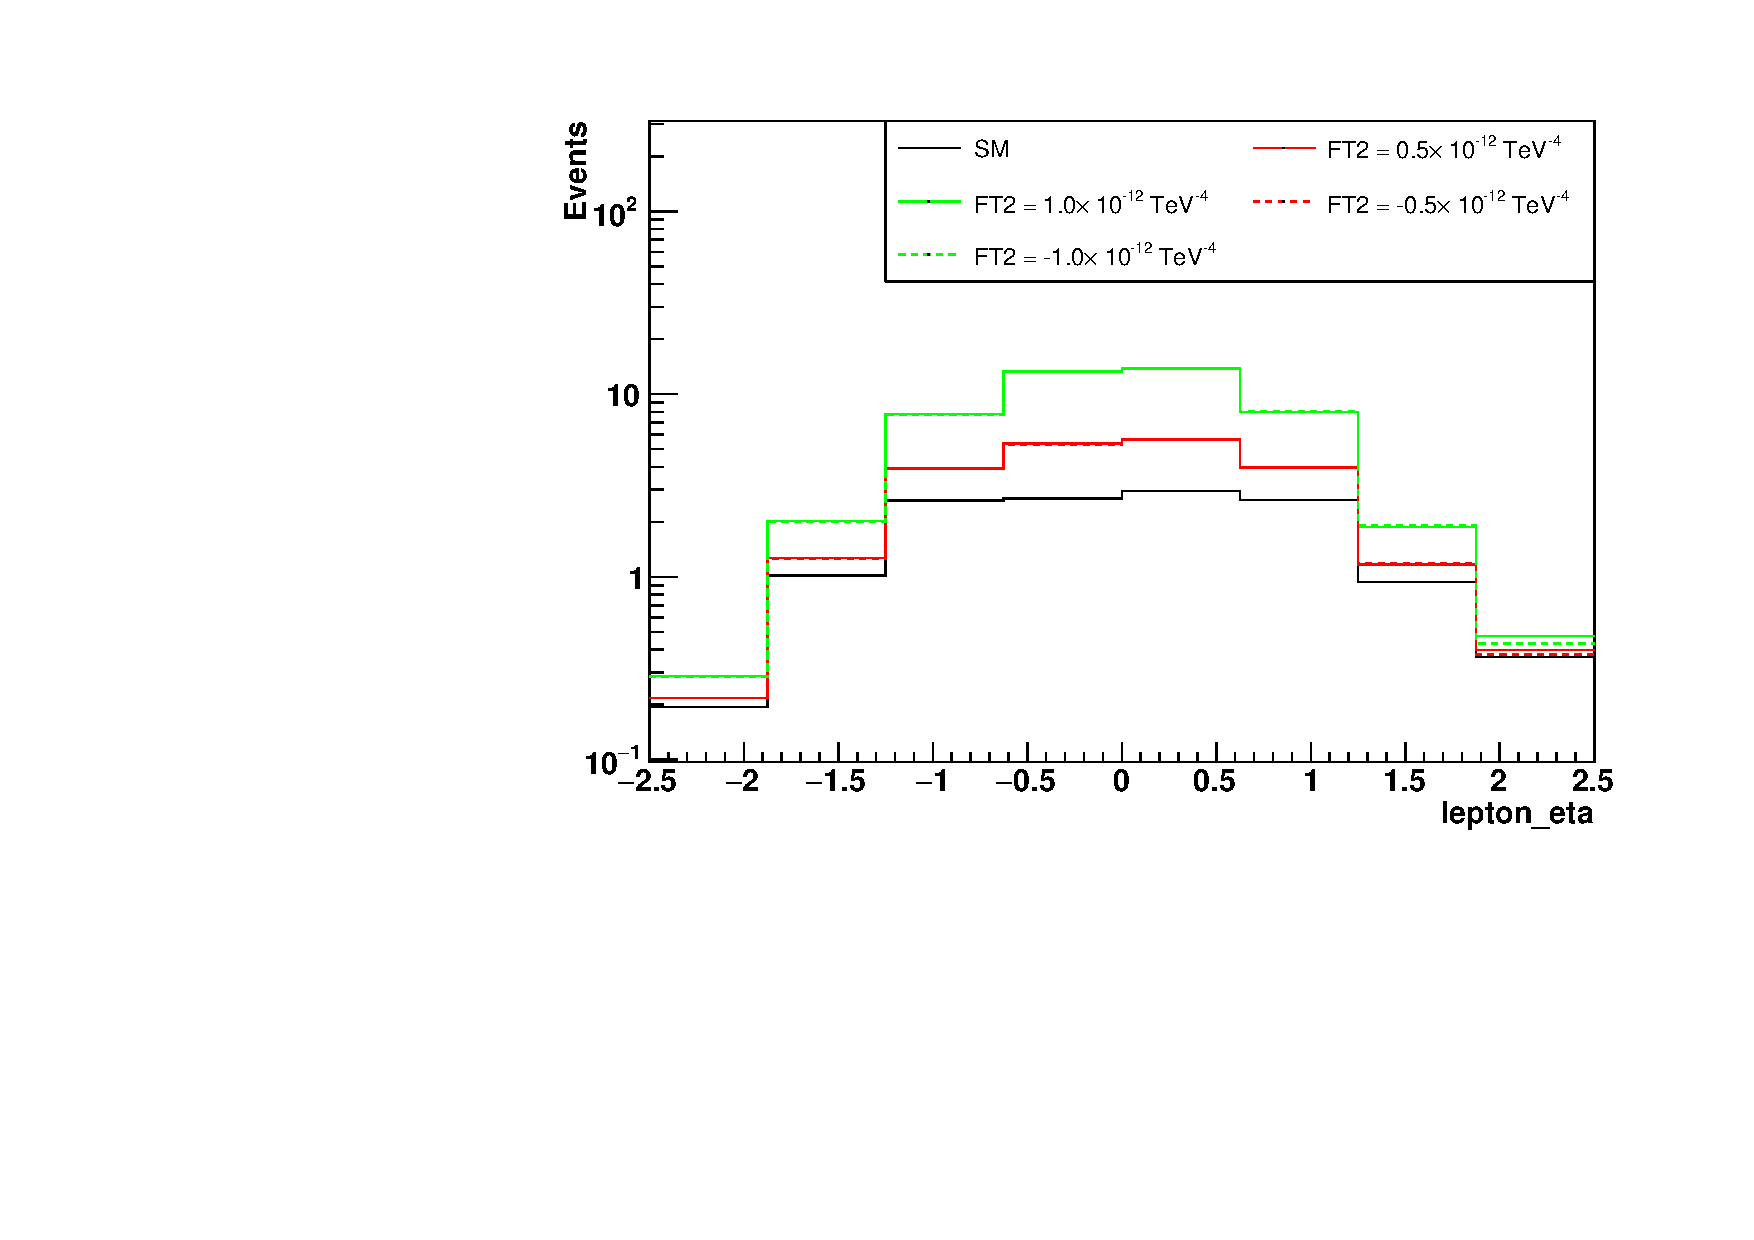
\includegraphics[width=0.45\textwidth]{Plots/aQGC_kinematics/lepton_eta_FT2_log.pdf}\\				
    \caption{}
  \end{center}
\end{figure}

\begin{figure}[h]
  \begin{center}
	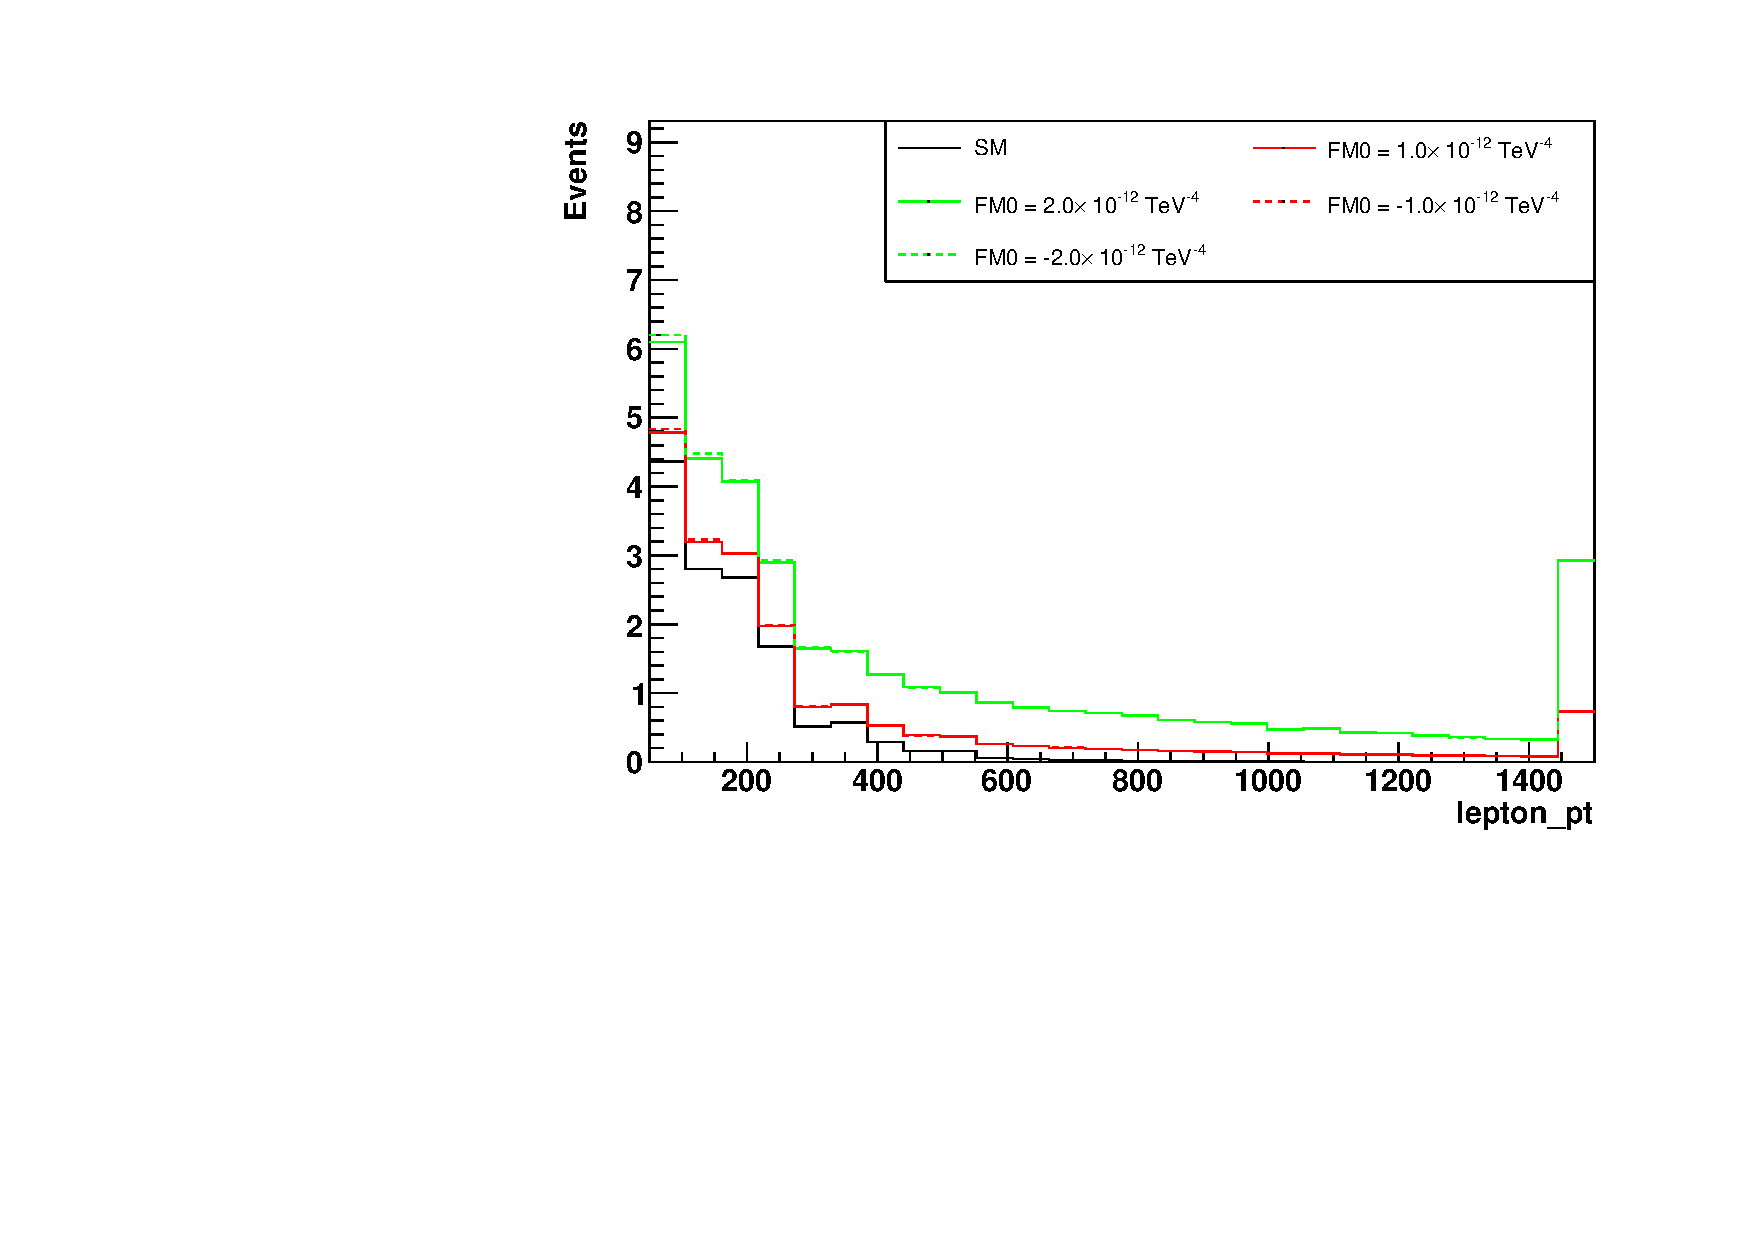
\includegraphics[width=0.45\textwidth]{Plots/aQGC_kinematics/lepton_pt_FM0.pdf}%	
	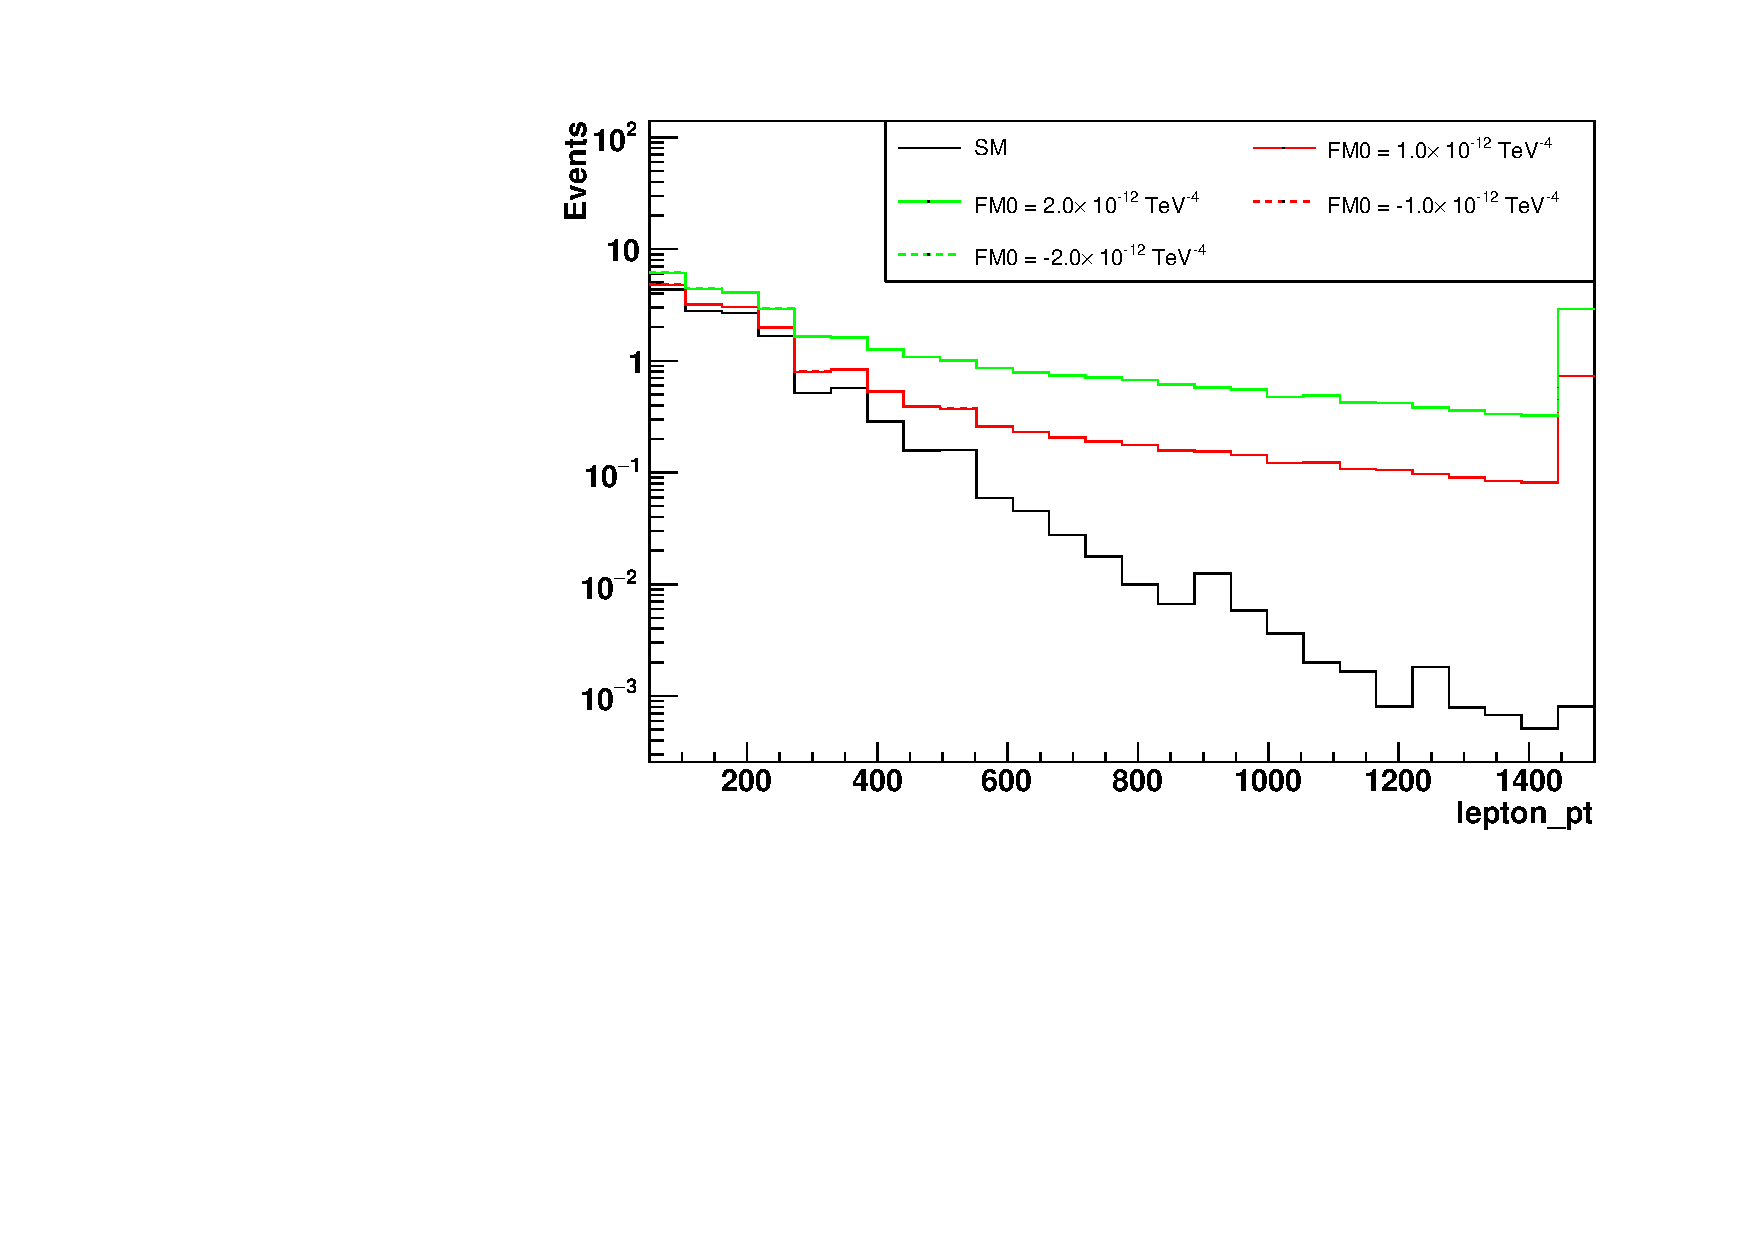
\includegraphics[width=0.45\textwidth]{Plots/aQGC_kinematics/lepton_pt_FM0_log.pdf}\\				
    \caption{}
  \end{center}
\end{figure}

\begin{figure}[h]
  \begin{center}
	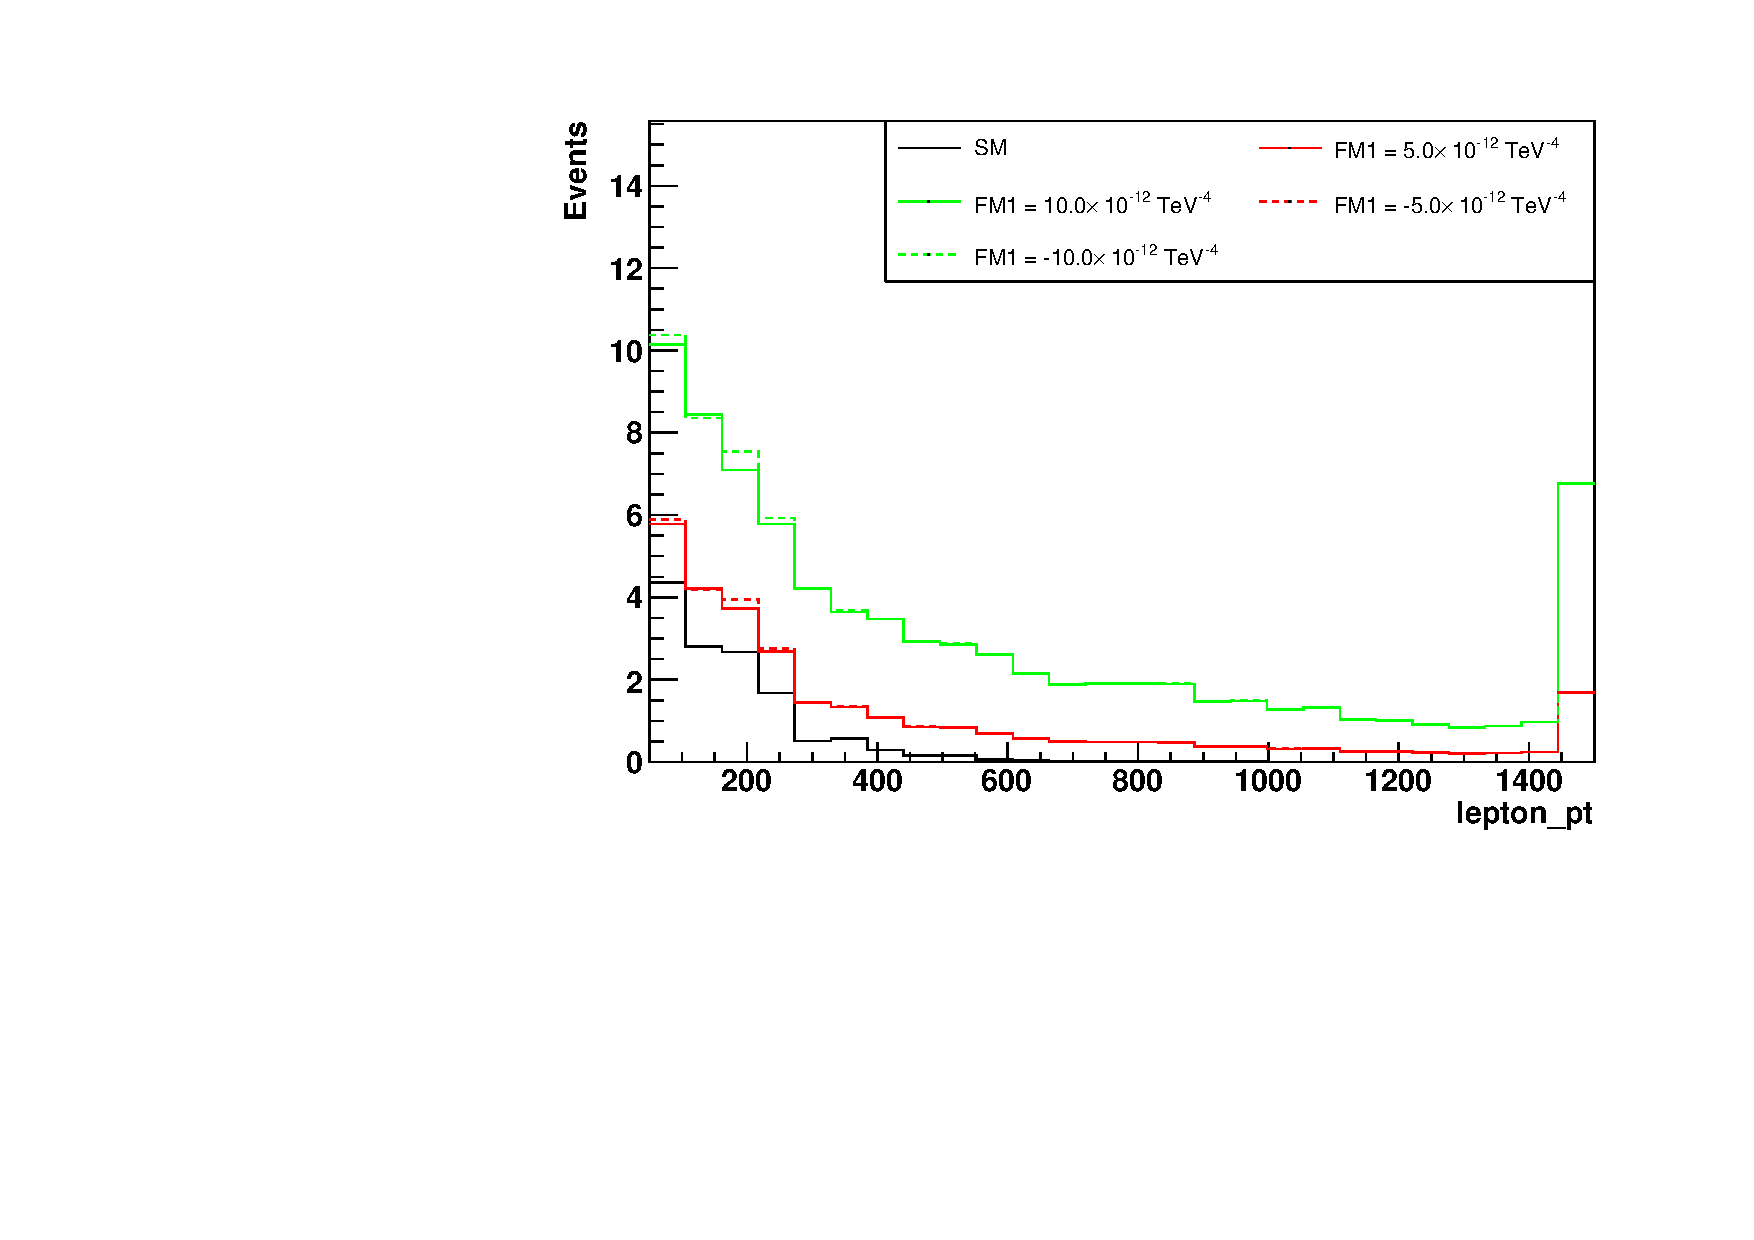
\includegraphics[width=0.45\textwidth]{Plots/aQGC_kinematics/lepton_pt_FM1.pdf}%	
	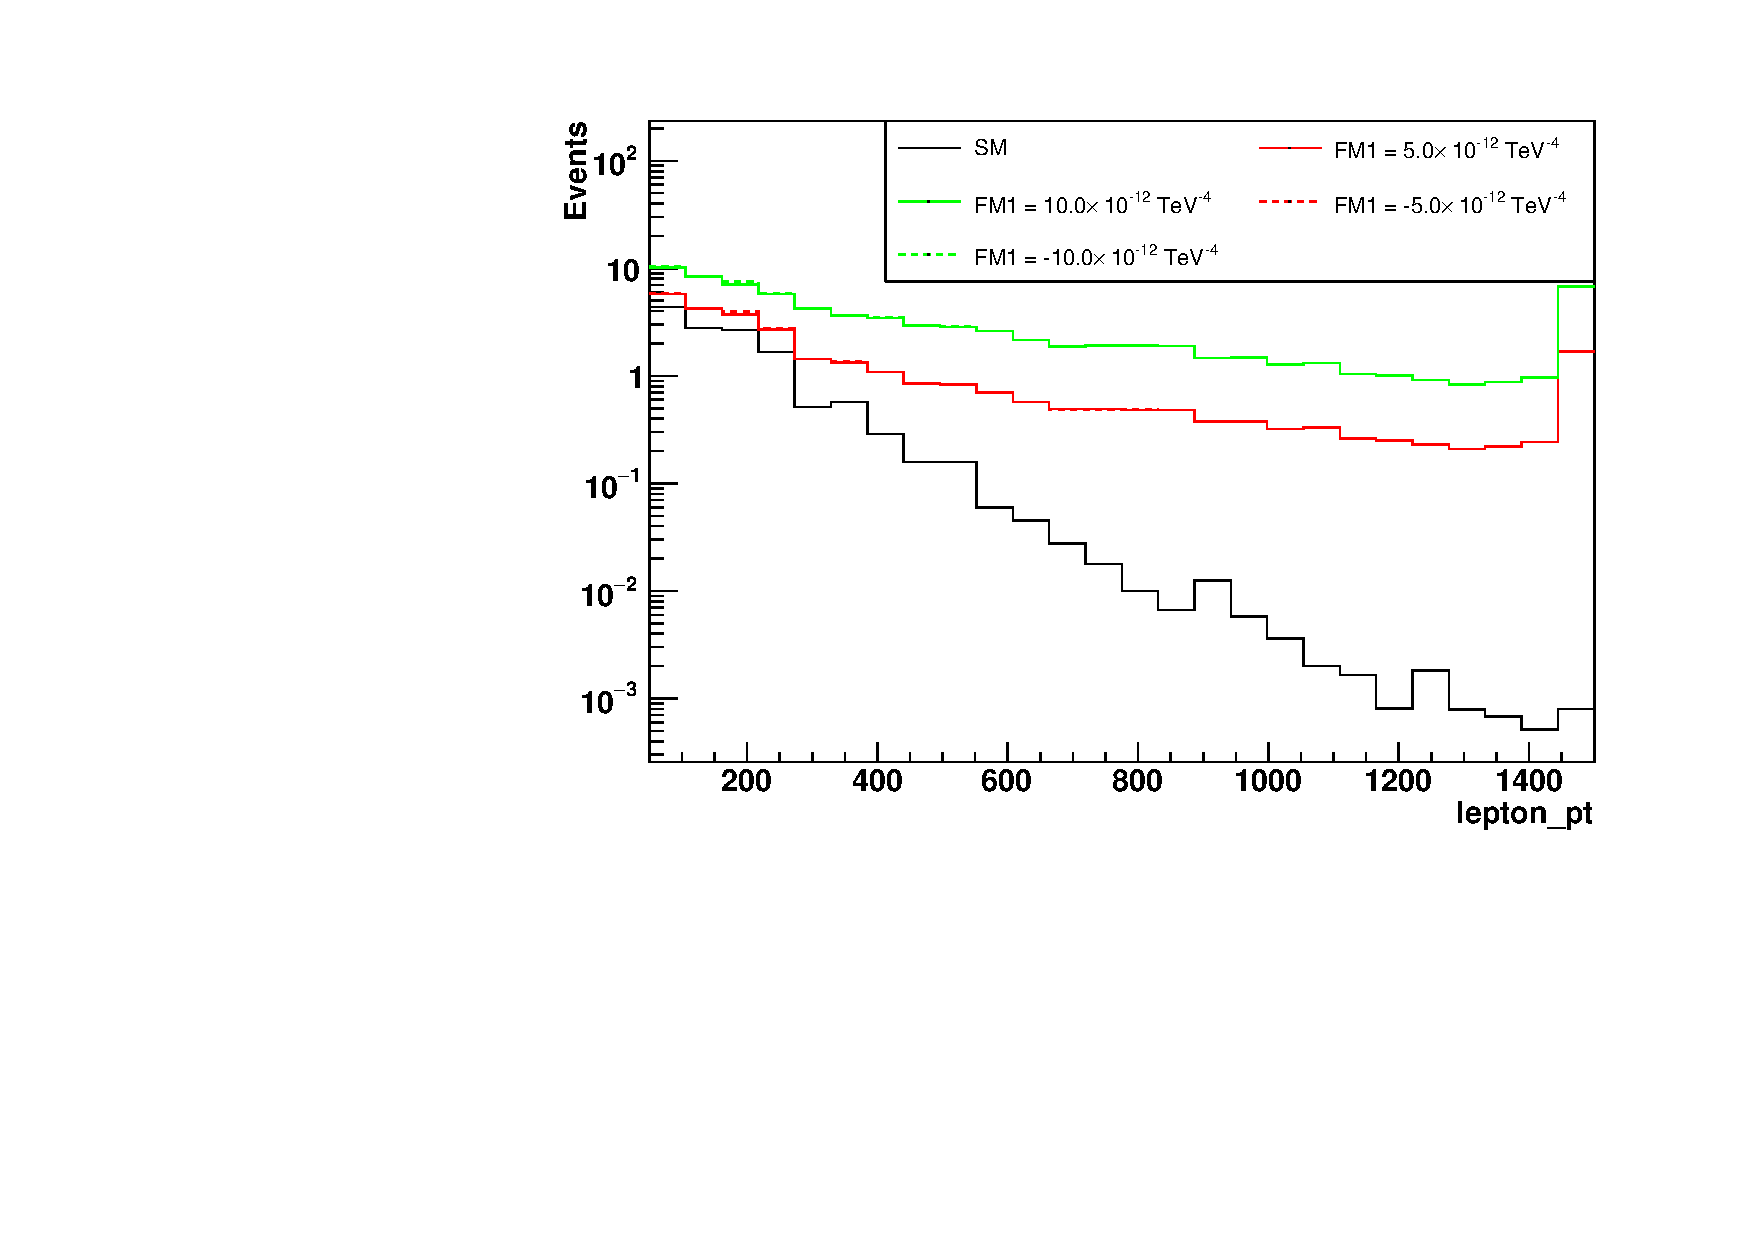
\includegraphics[width=0.45\textwidth]{Plots/aQGC_kinematics/lepton_pt_FM1_log.pdf}\\				
    \caption{}
  \end{center}
\end{figure}

\begin{figure}[h]
  \begin{center}
	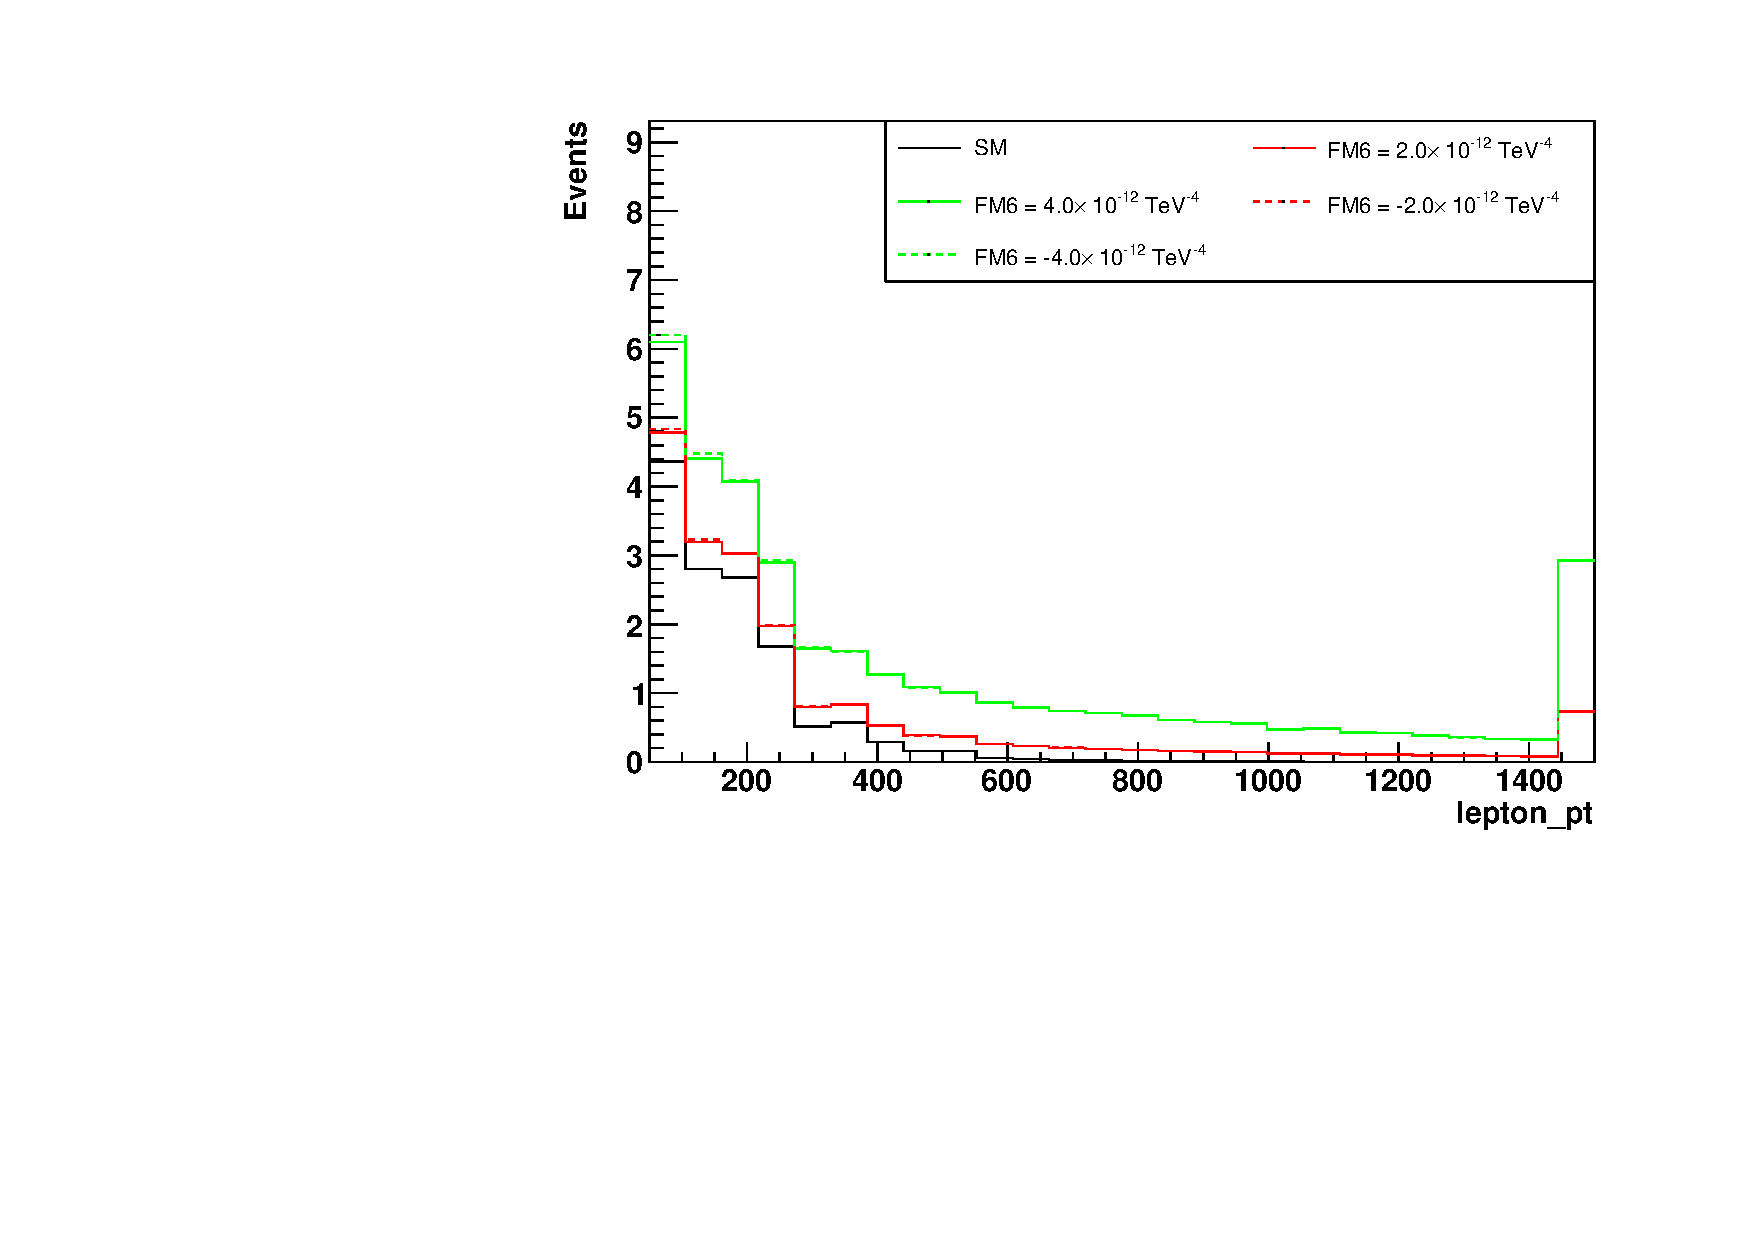
\includegraphics[width=0.45\textwidth]{Plots/aQGC_kinematics/lepton_pt_FM6.pdf}%	
	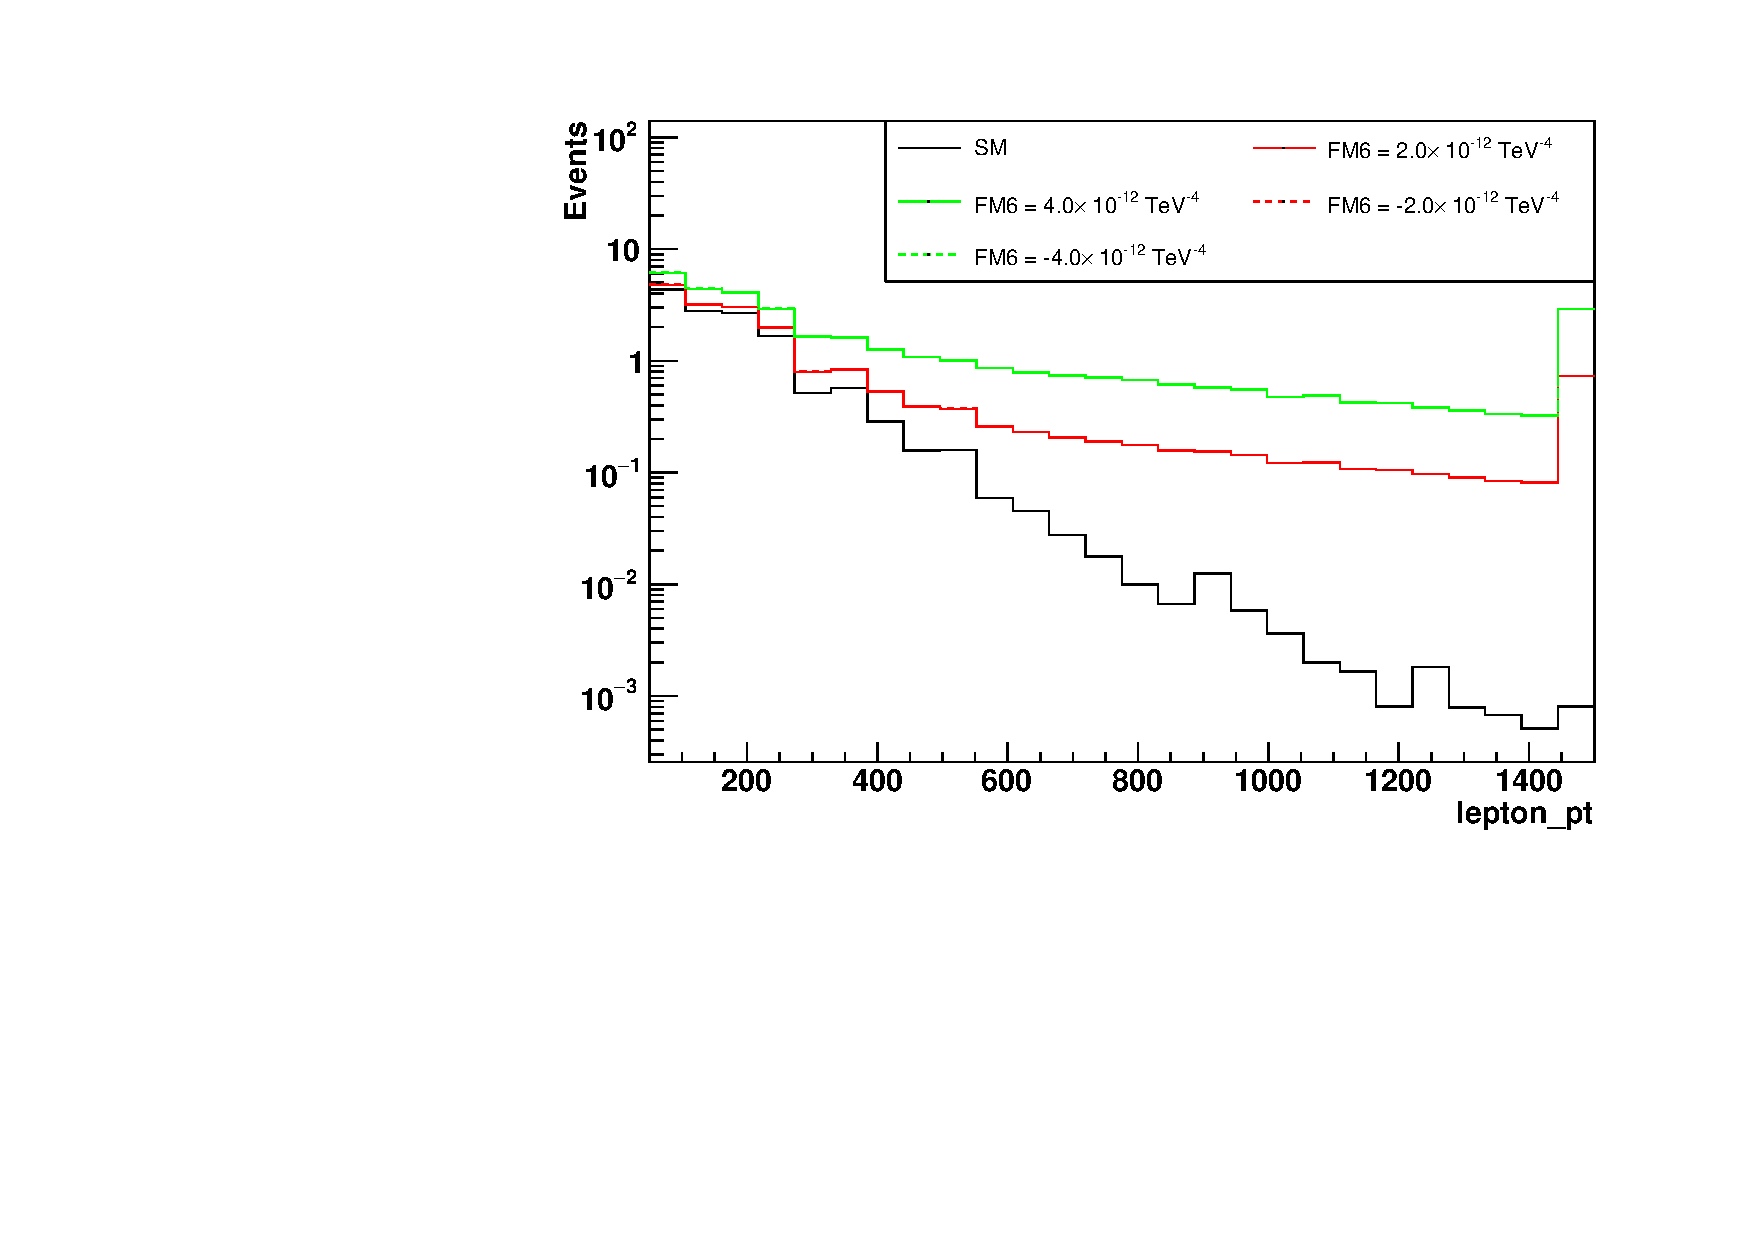
\includegraphics[width=0.45\textwidth]{Plots/aQGC_kinematics/lepton_pt_FM6_log.pdf}\\				
    \caption{}
  \end{center}
\end{figure}

\begin{figure}[h]
  \begin{center}
	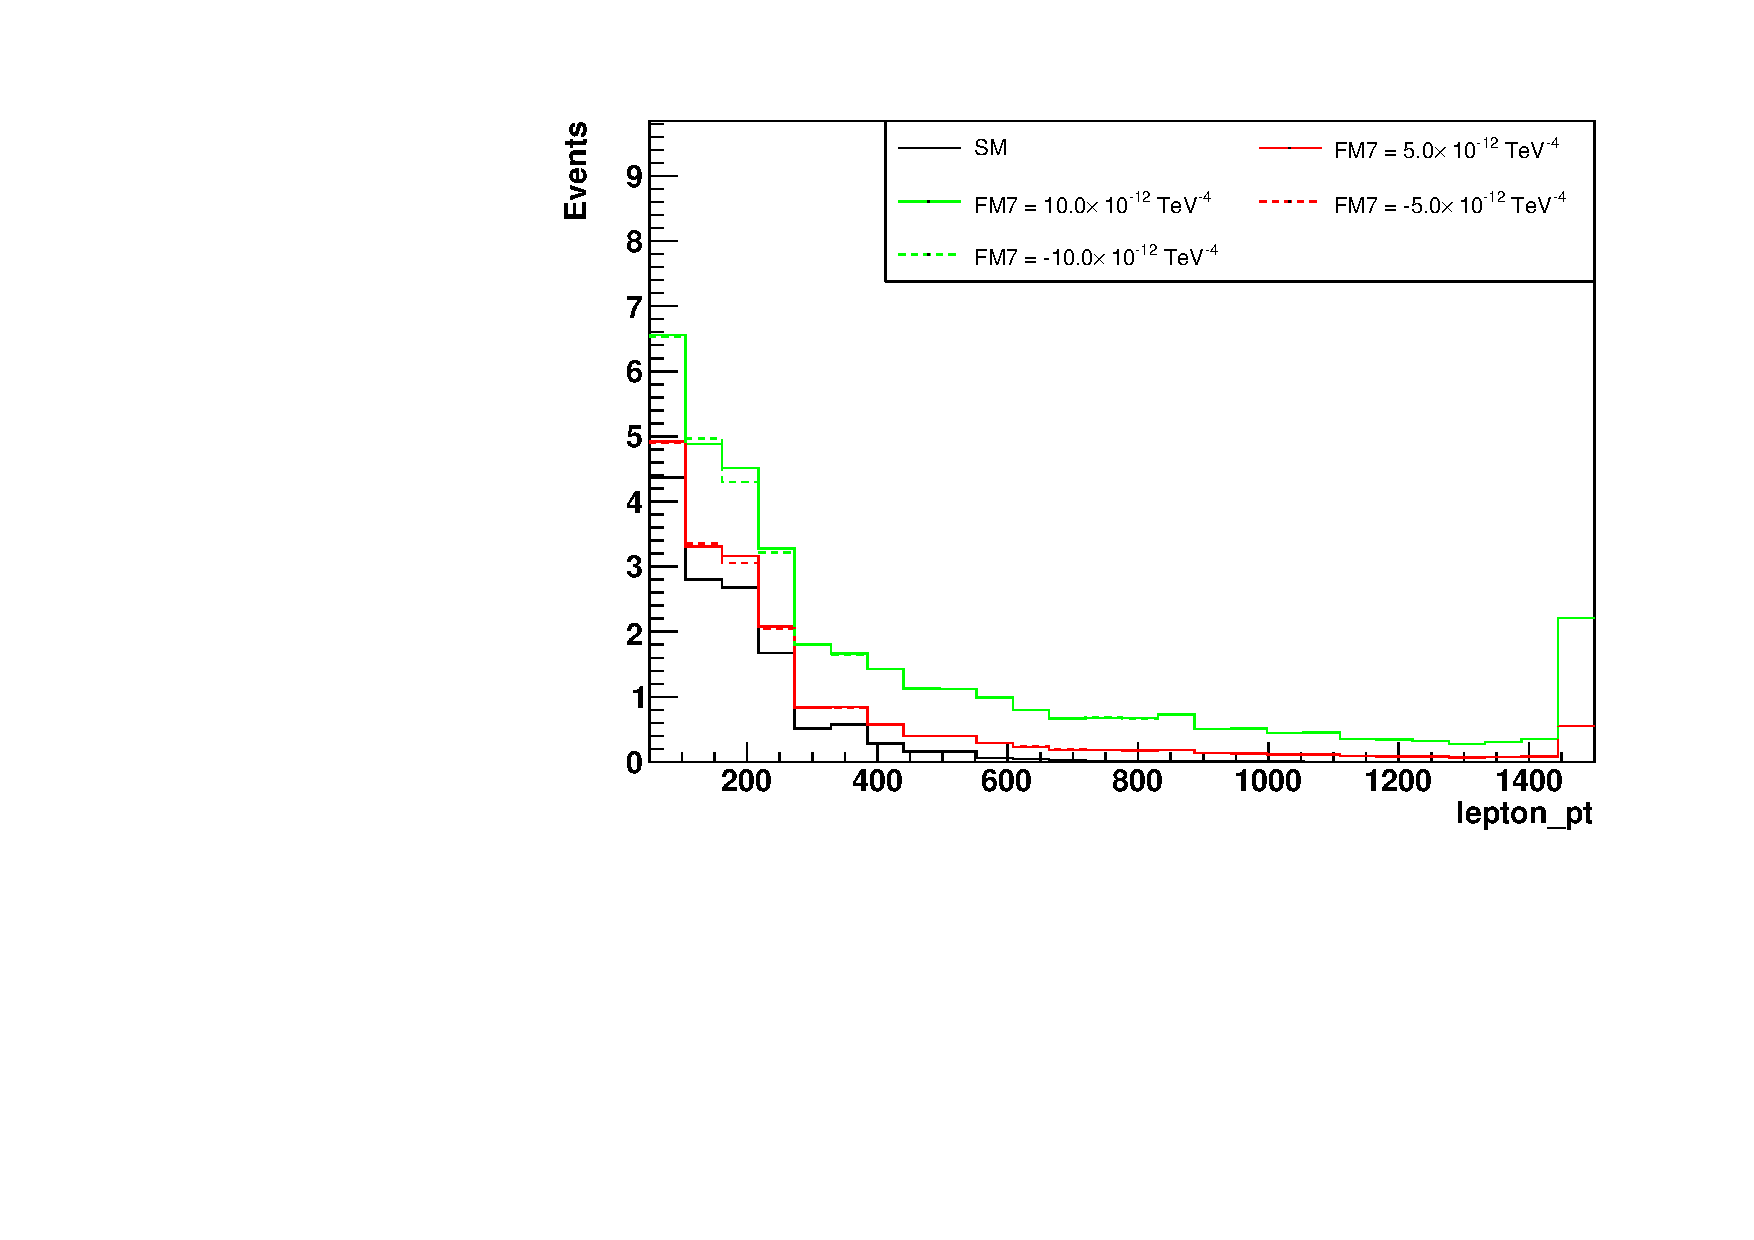
\includegraphics[width=0.45\textwidth]{Plots/aQGC_kinematics/lepton_pt_FM7.pdf}%	
	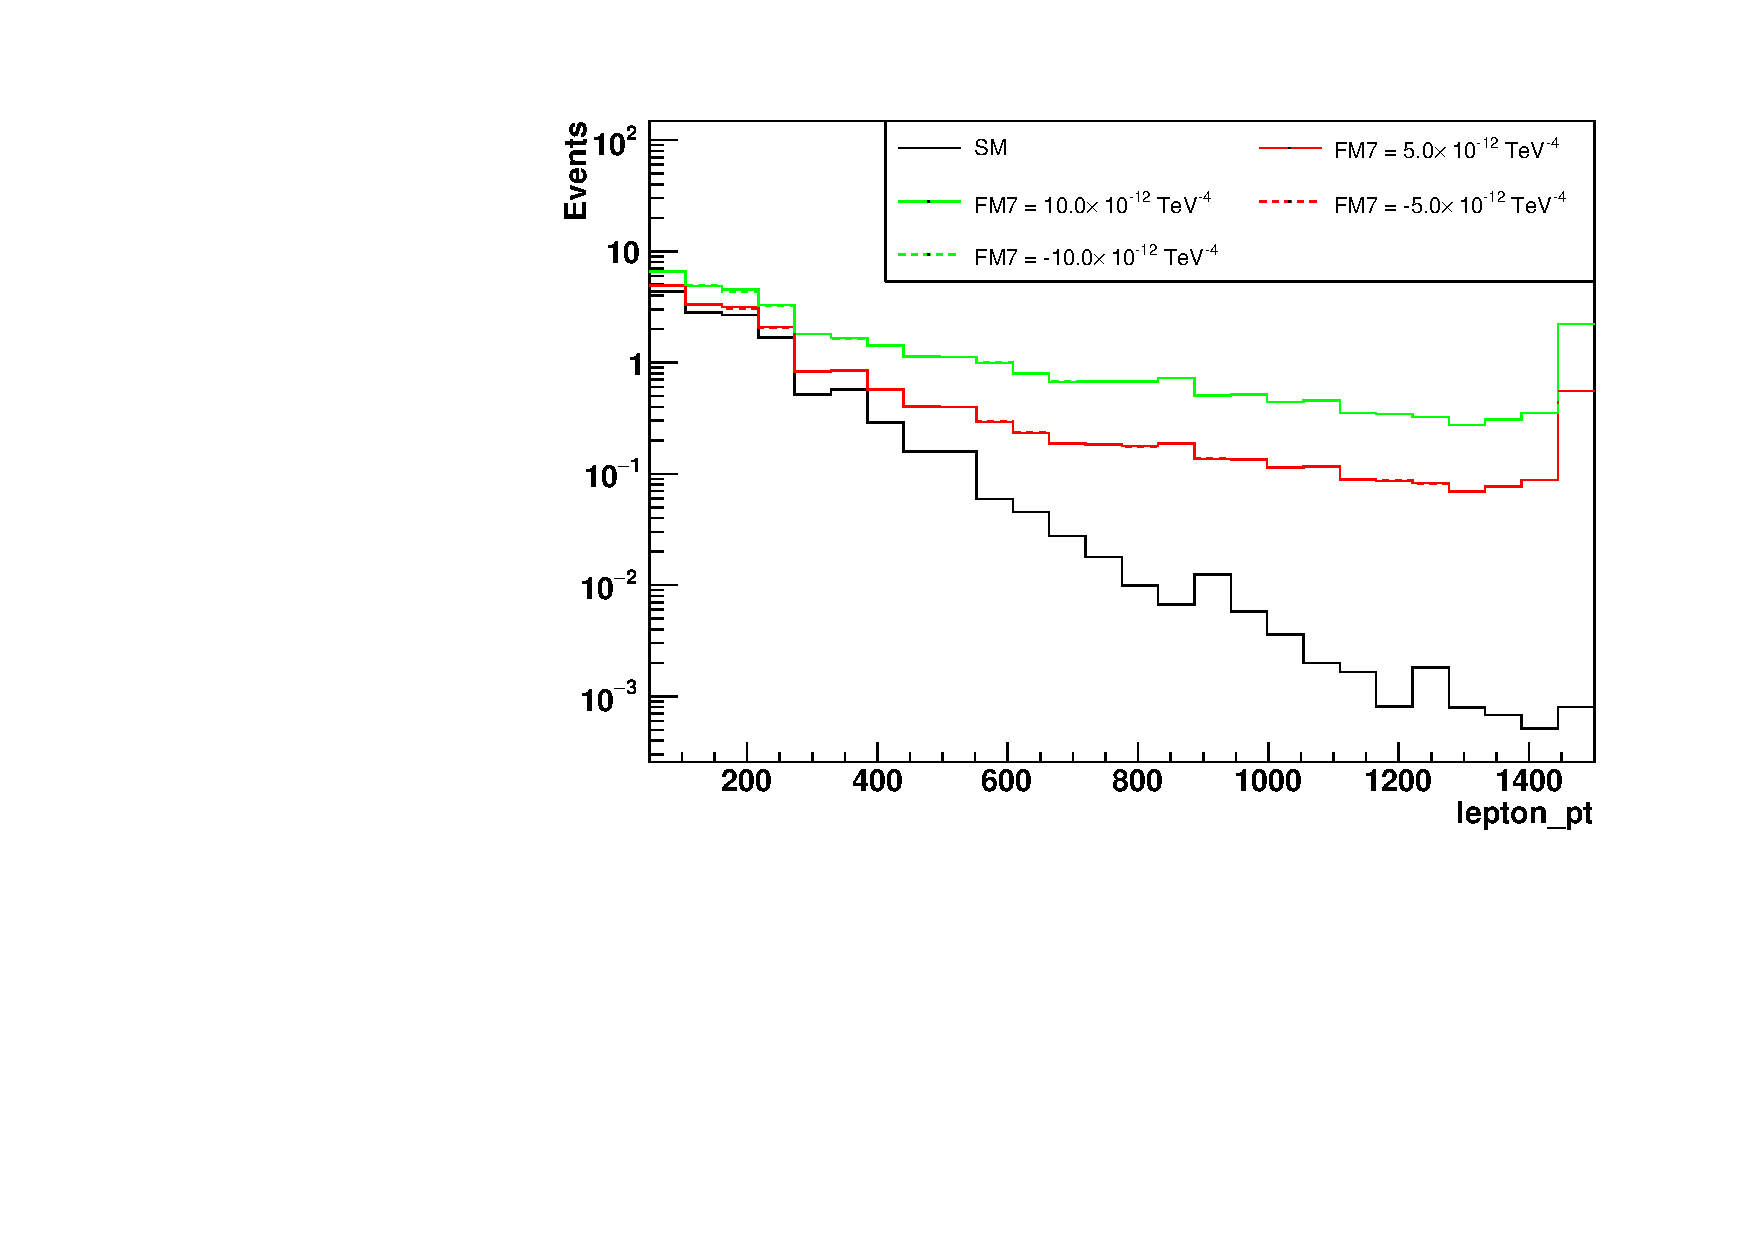
\includegraphics[width=0.45\textwidth]{Plots/aQGC_kinematics/lepton_pt_FM7_log.pdf}\\				
    \caption{}
  \end{center}
\end{figure}

\begin{figure}[h]
  \begin{center}
	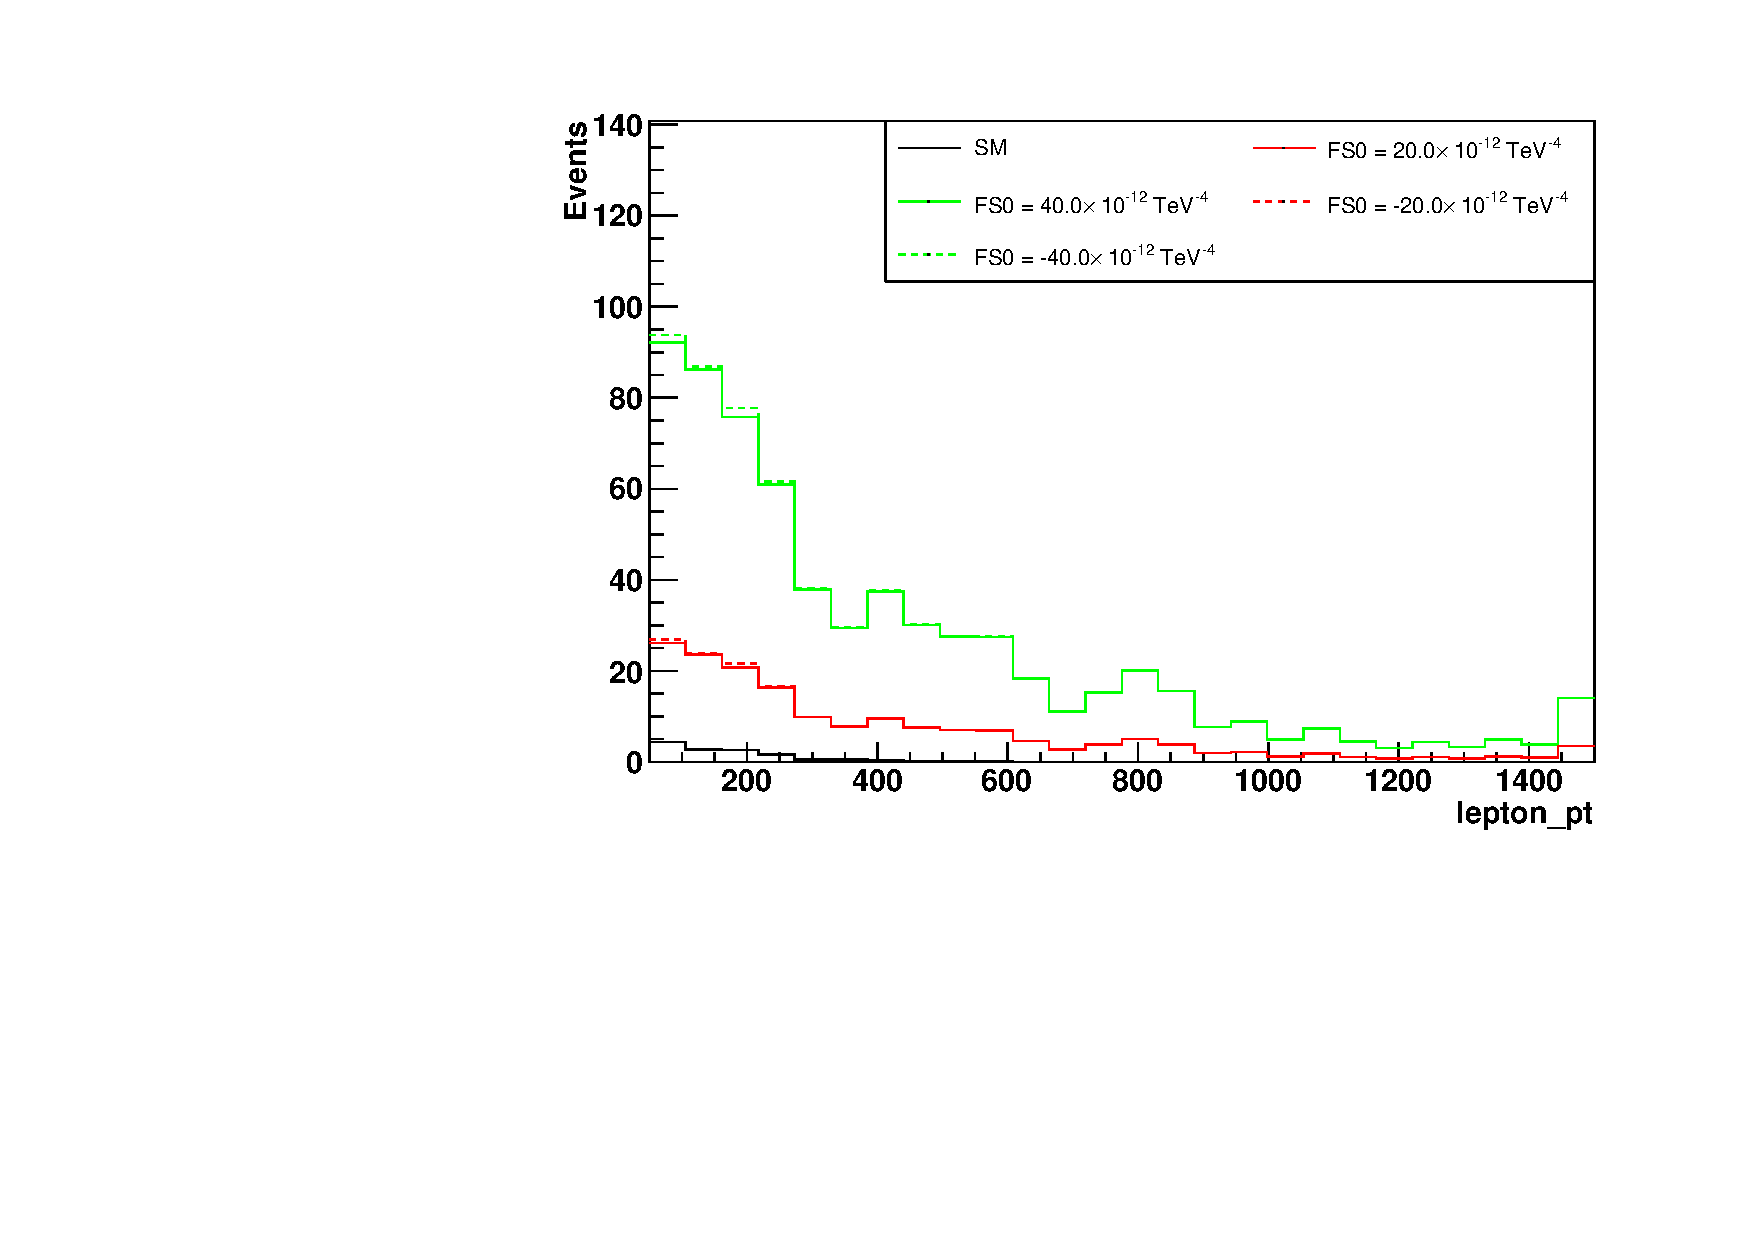
\includegraphics[width=0.45\textwidth]{Plots/aQGC_kinematics/lepton_pt_FS0.pdf}%	
	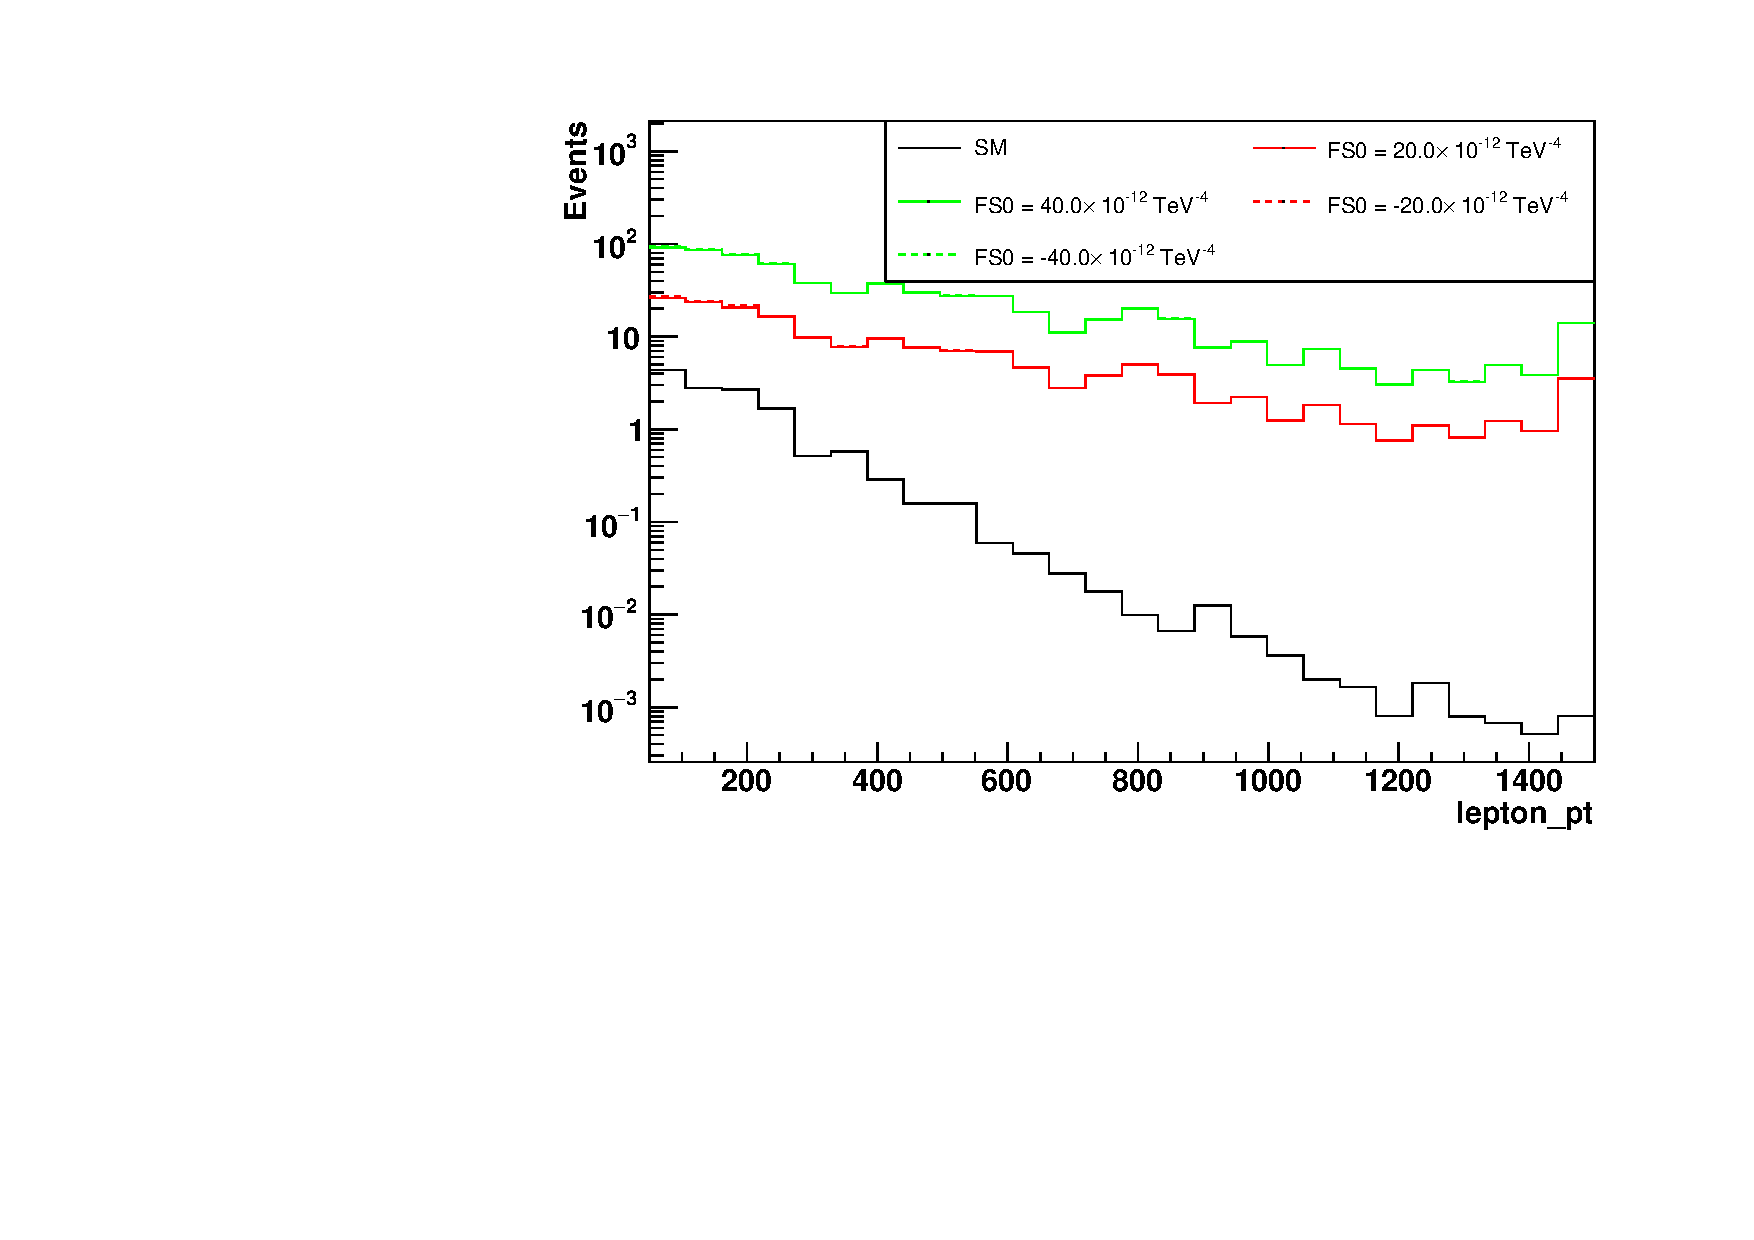
\includegraphics[width=0.45\textwidth]{Plots/aQGC_kinematics/lepton_pt_FS0_log.pdf}\\				
    \caption{}
  \end{center}
\end{figure}

\begin{figure}[h]
  \begin{center}
	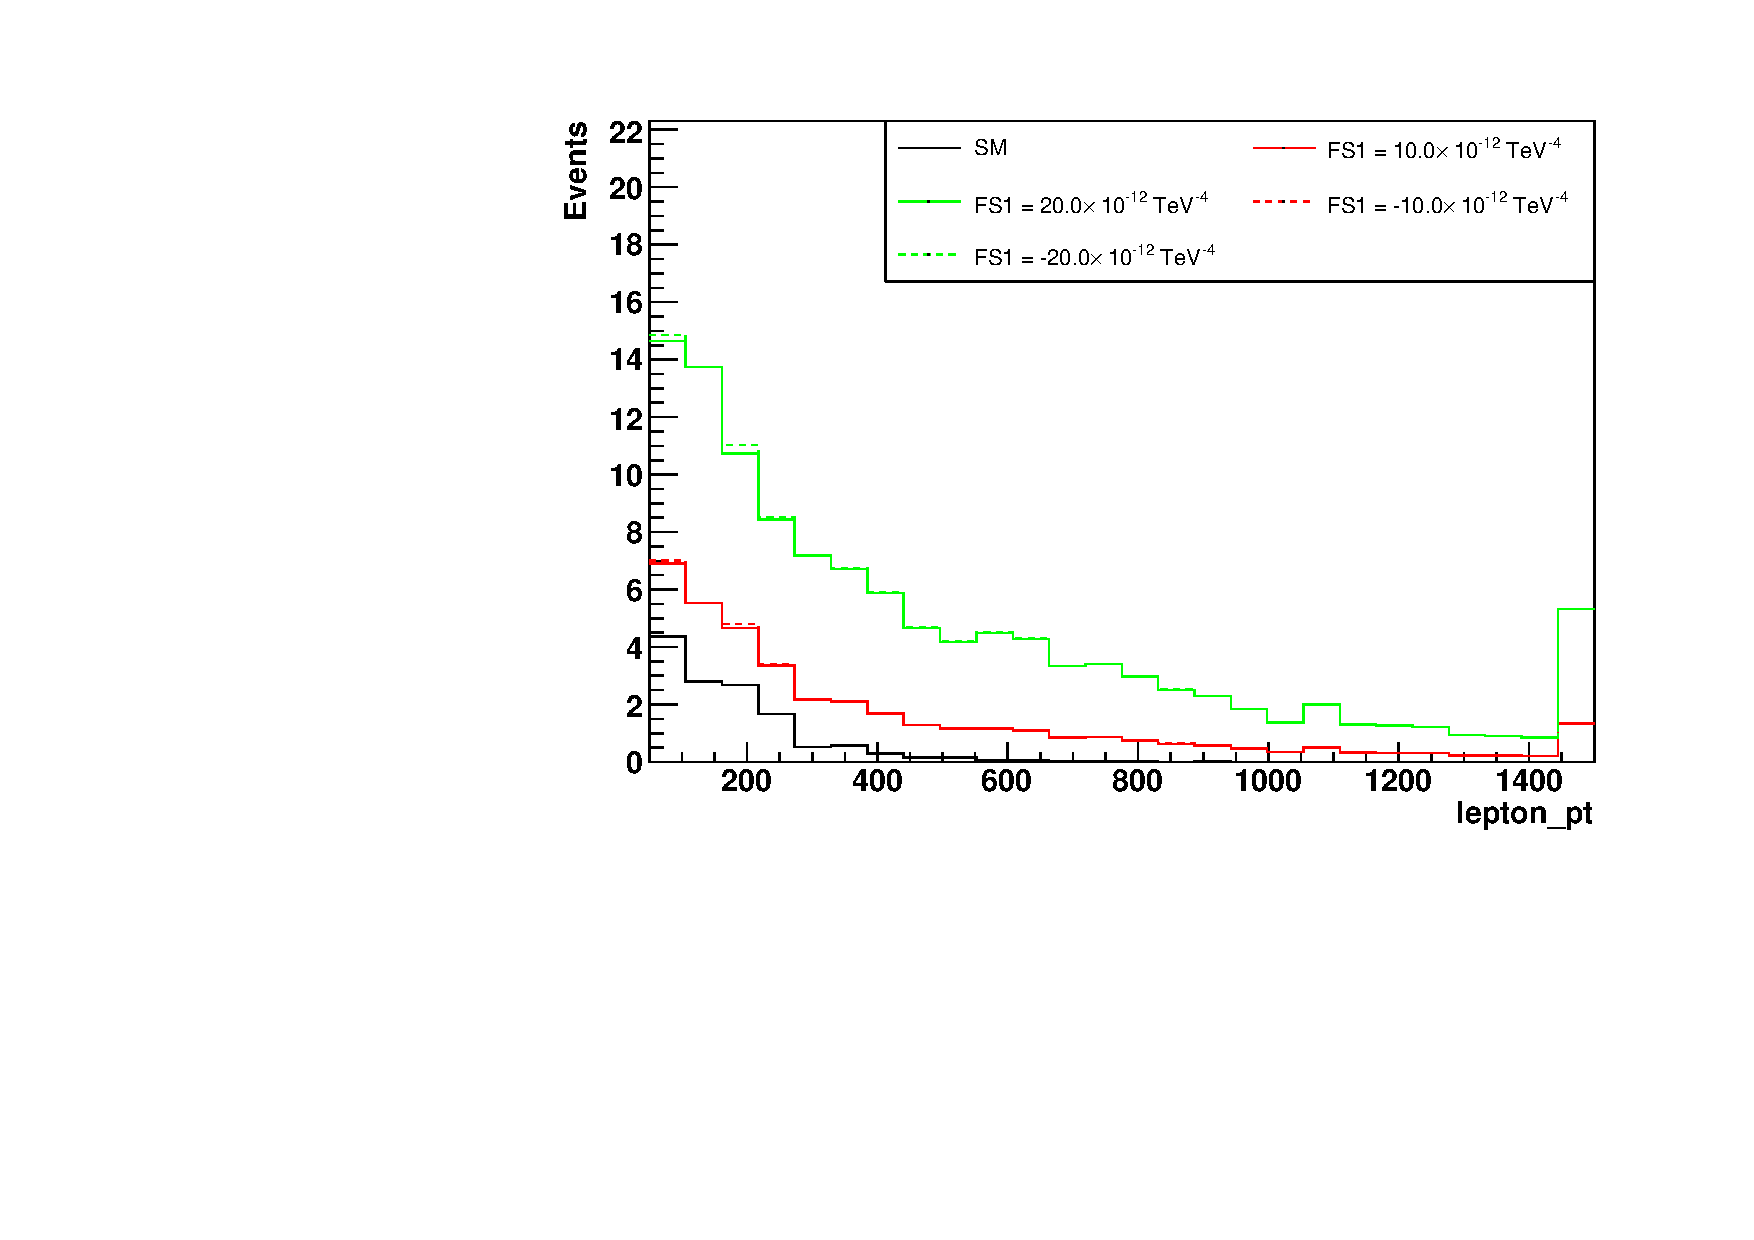
\includegraphics[width=0.45\textwidth]{Plots/aQGC_kinematics/lepton_pt_FS1.pdf}%	
	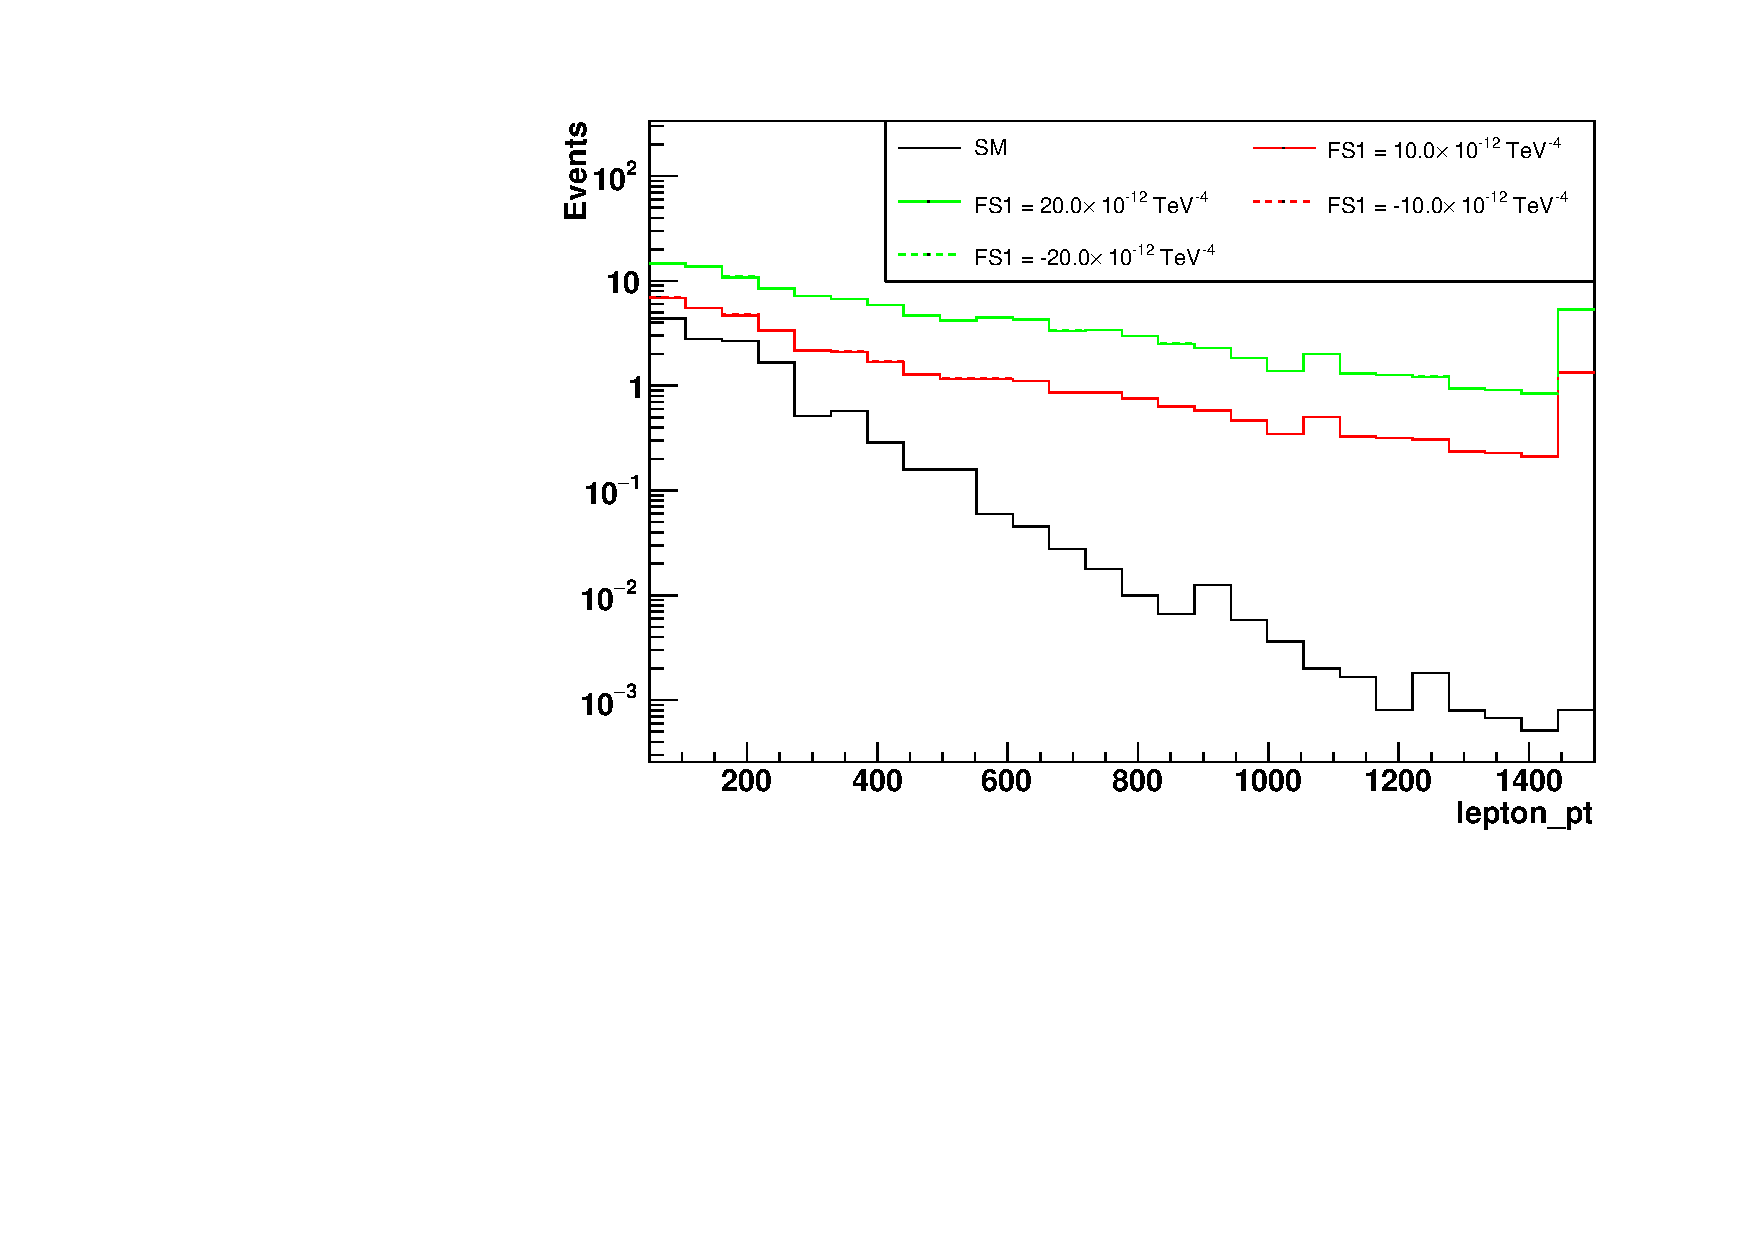
\includegraphics[width=0.45\textwidth]{Plots/aQGC_kinematics/lepton_pt_FS1_log.pdf}\\				
    \caption{}
  \end{center}
\end{figure}

\begin{figure}[h]
  \begin{center}
	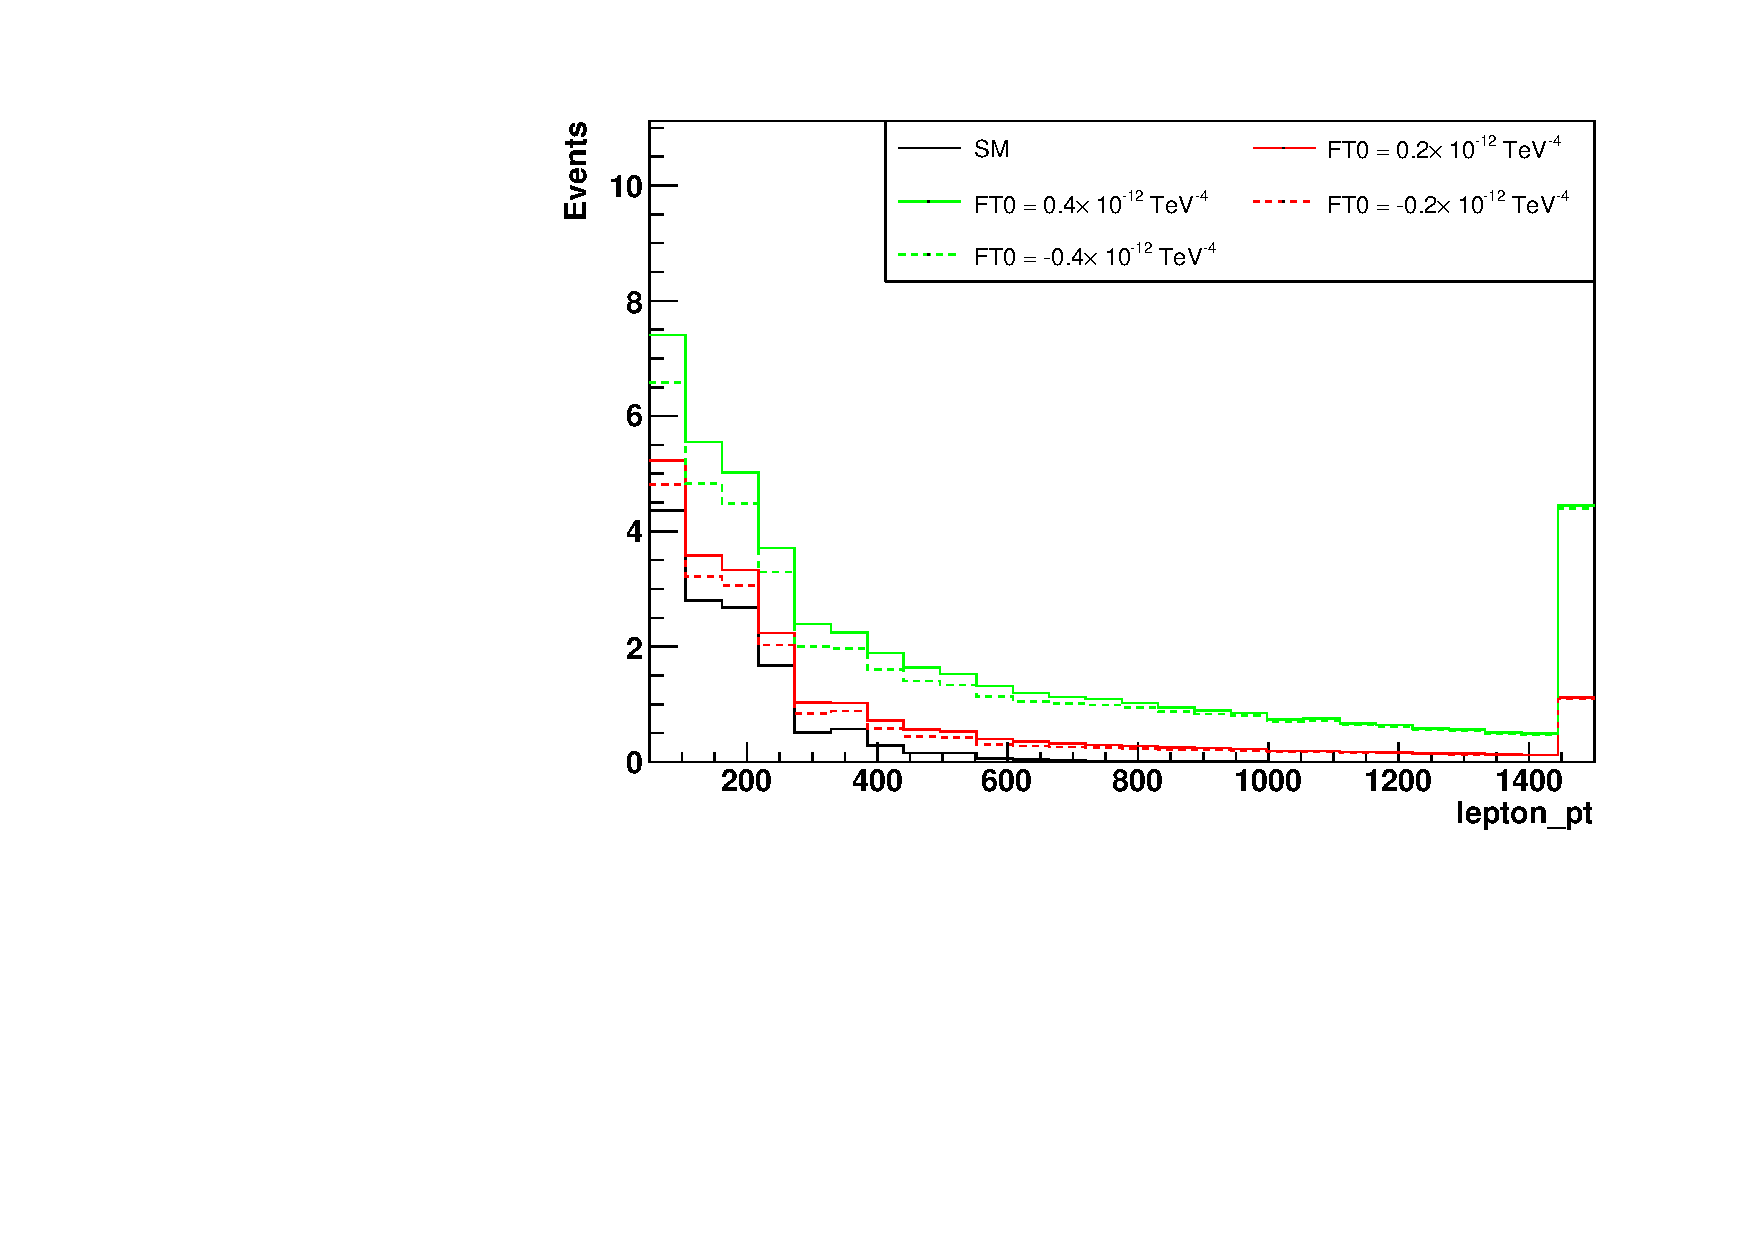
\includegraphics[width=0.45\textwidth]{Plots/aQGC_kinematics/lepton_pt_FT0.pdf}%	
	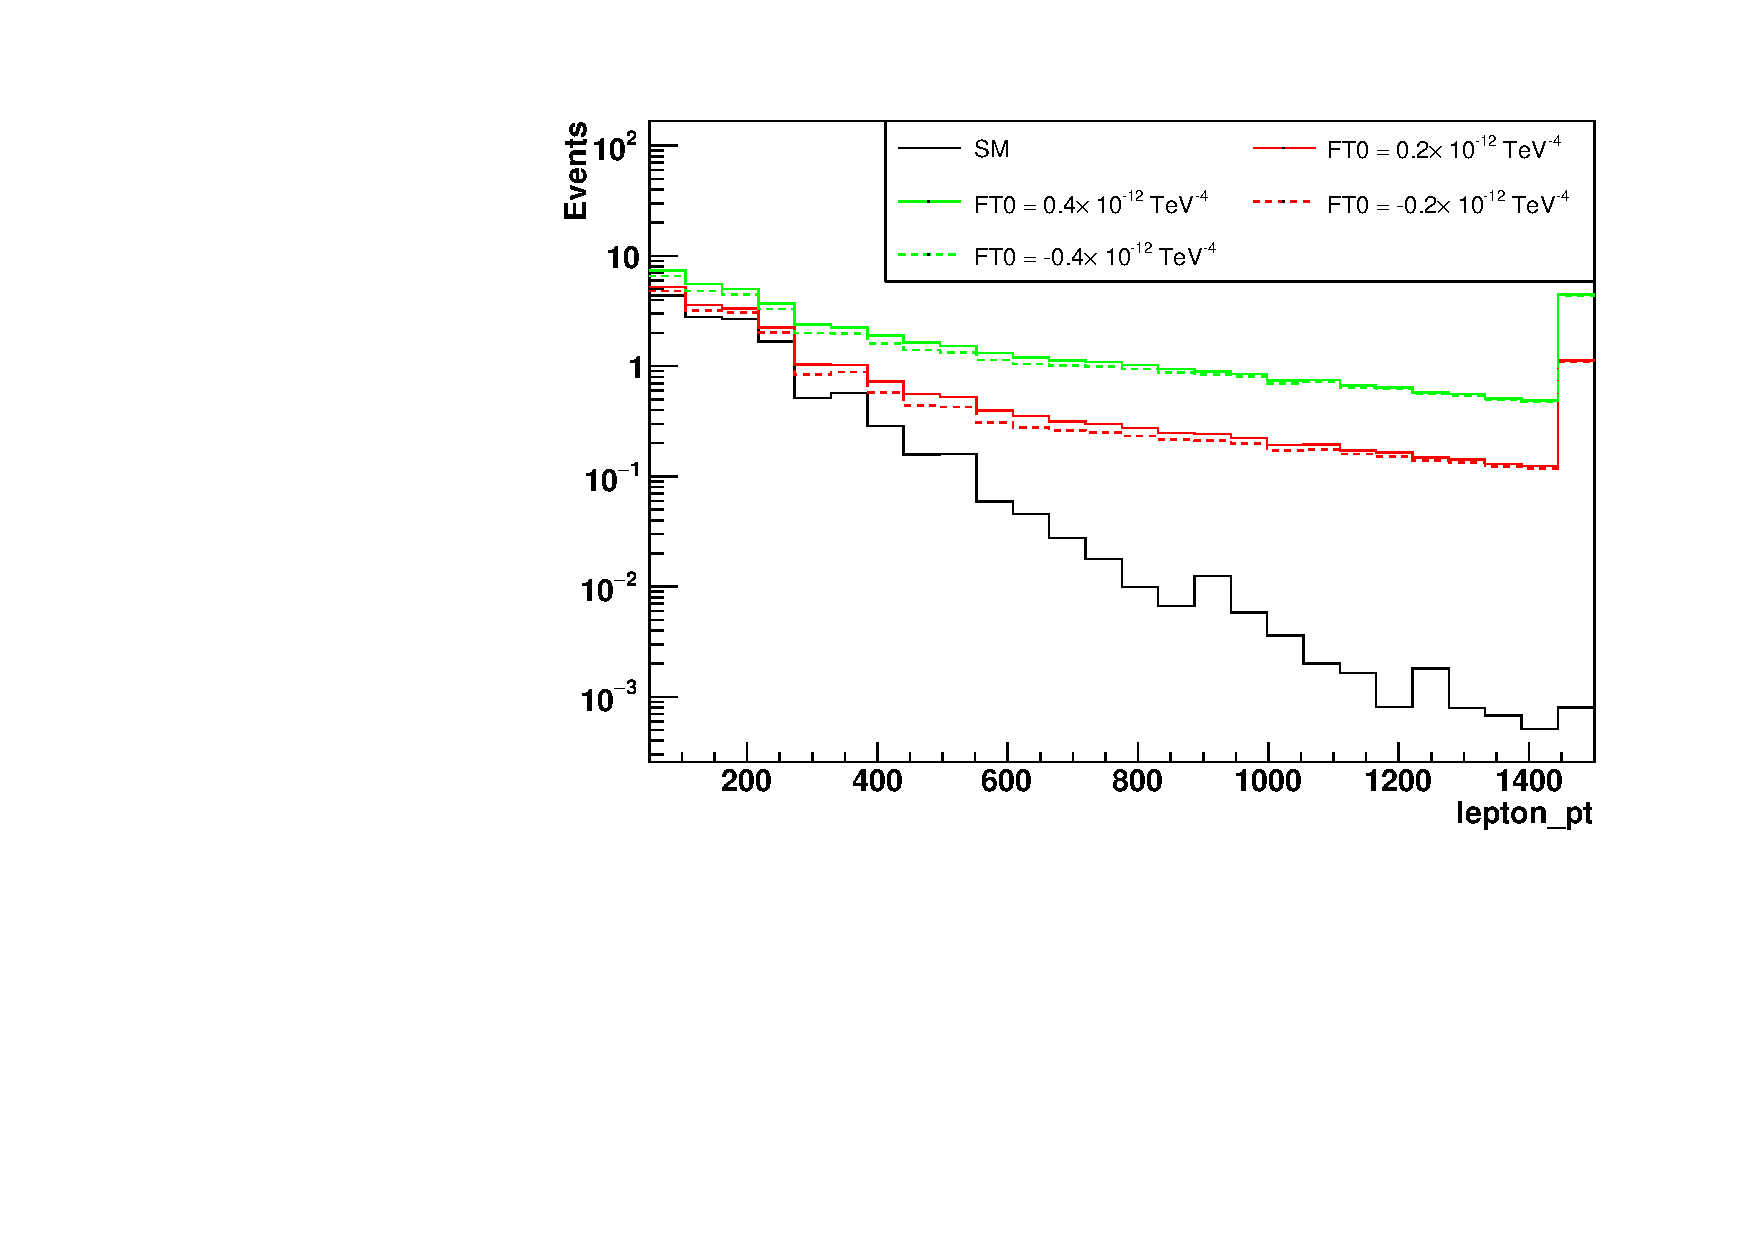
\includegraphics[width=0.45\textwidth]{Plots/aQGC_kinematics/lepton_pt_FT0_log.pdf}\\				
    \caption{}
  \end{center}
\end{figure}

\begin{figure}[h]
  \begin{center}
	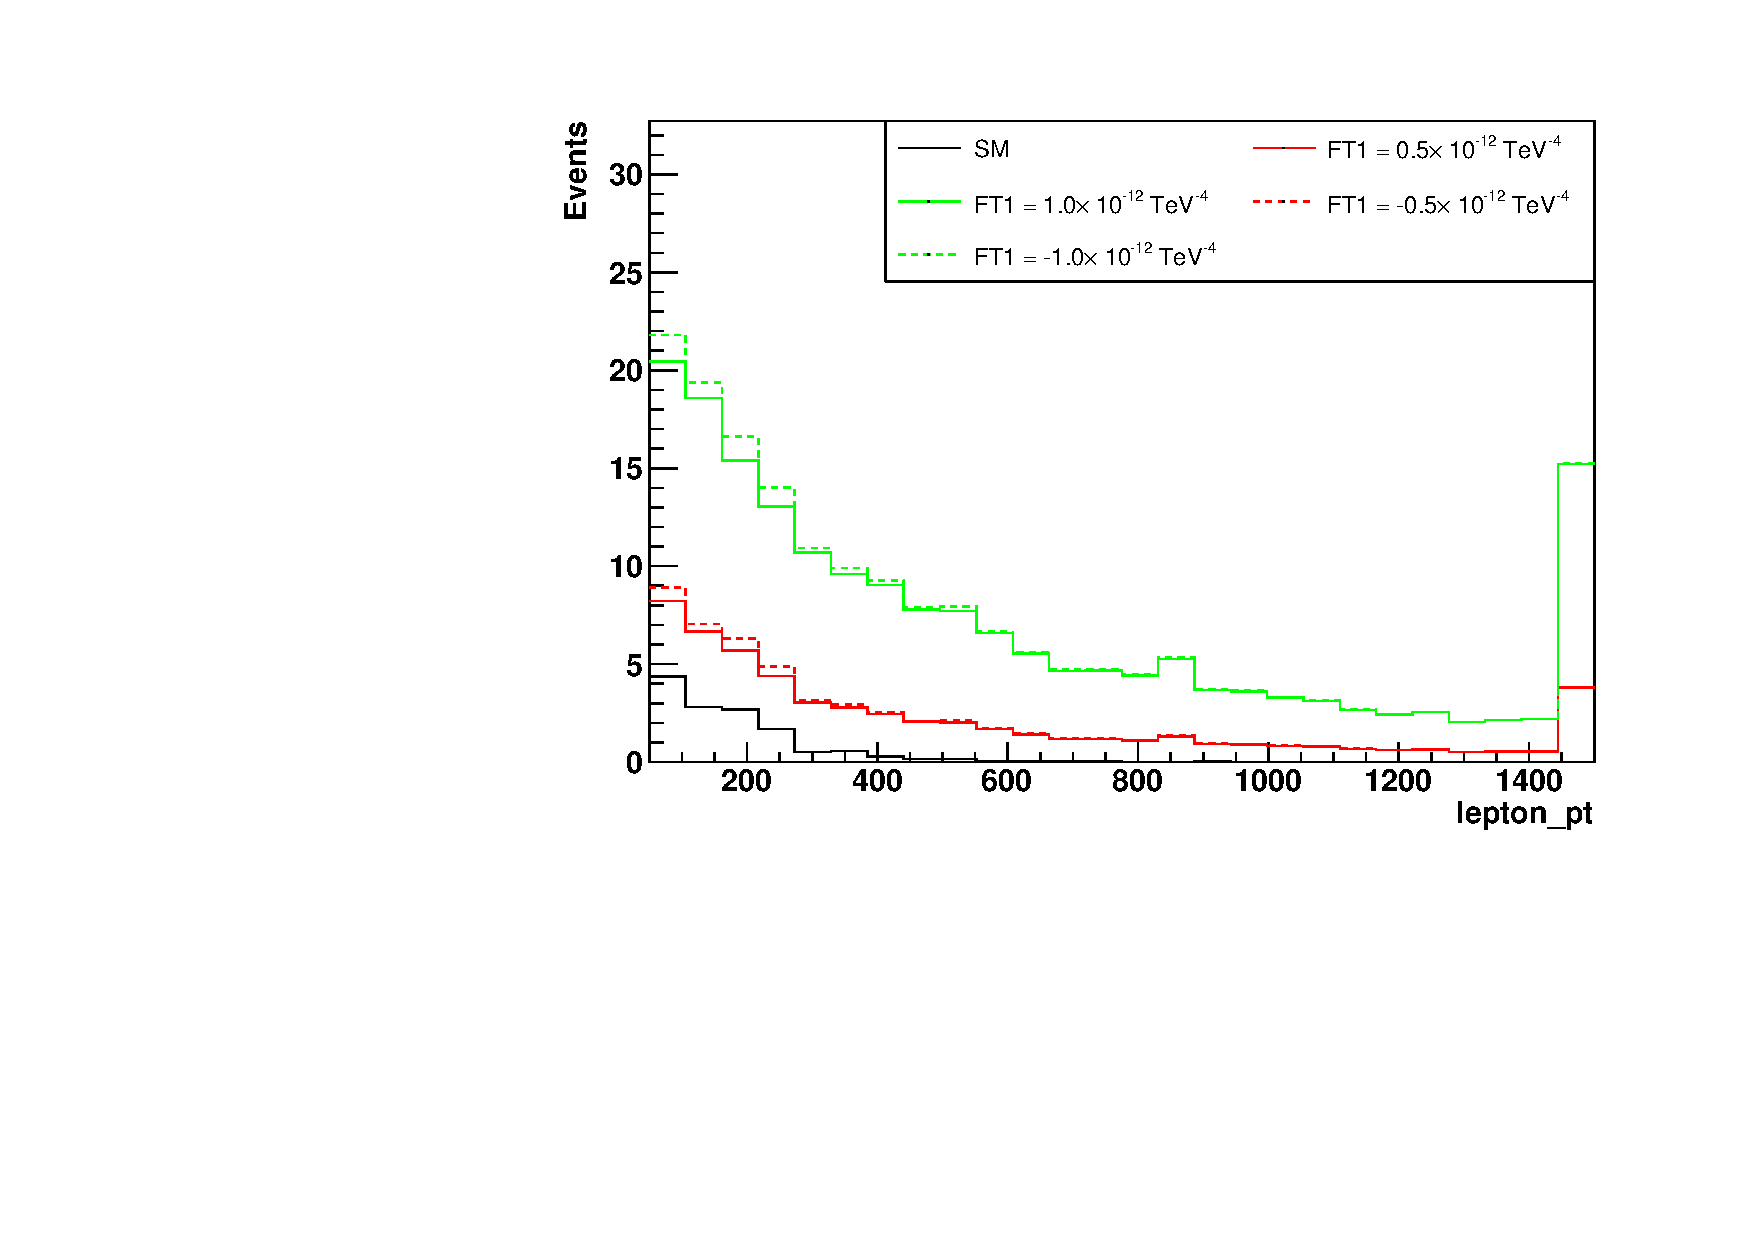
\includegraphics[width=0.45\textwidth]{Plots/aQGC_kinematics/lepton_pt_FT1.pdf}%	
	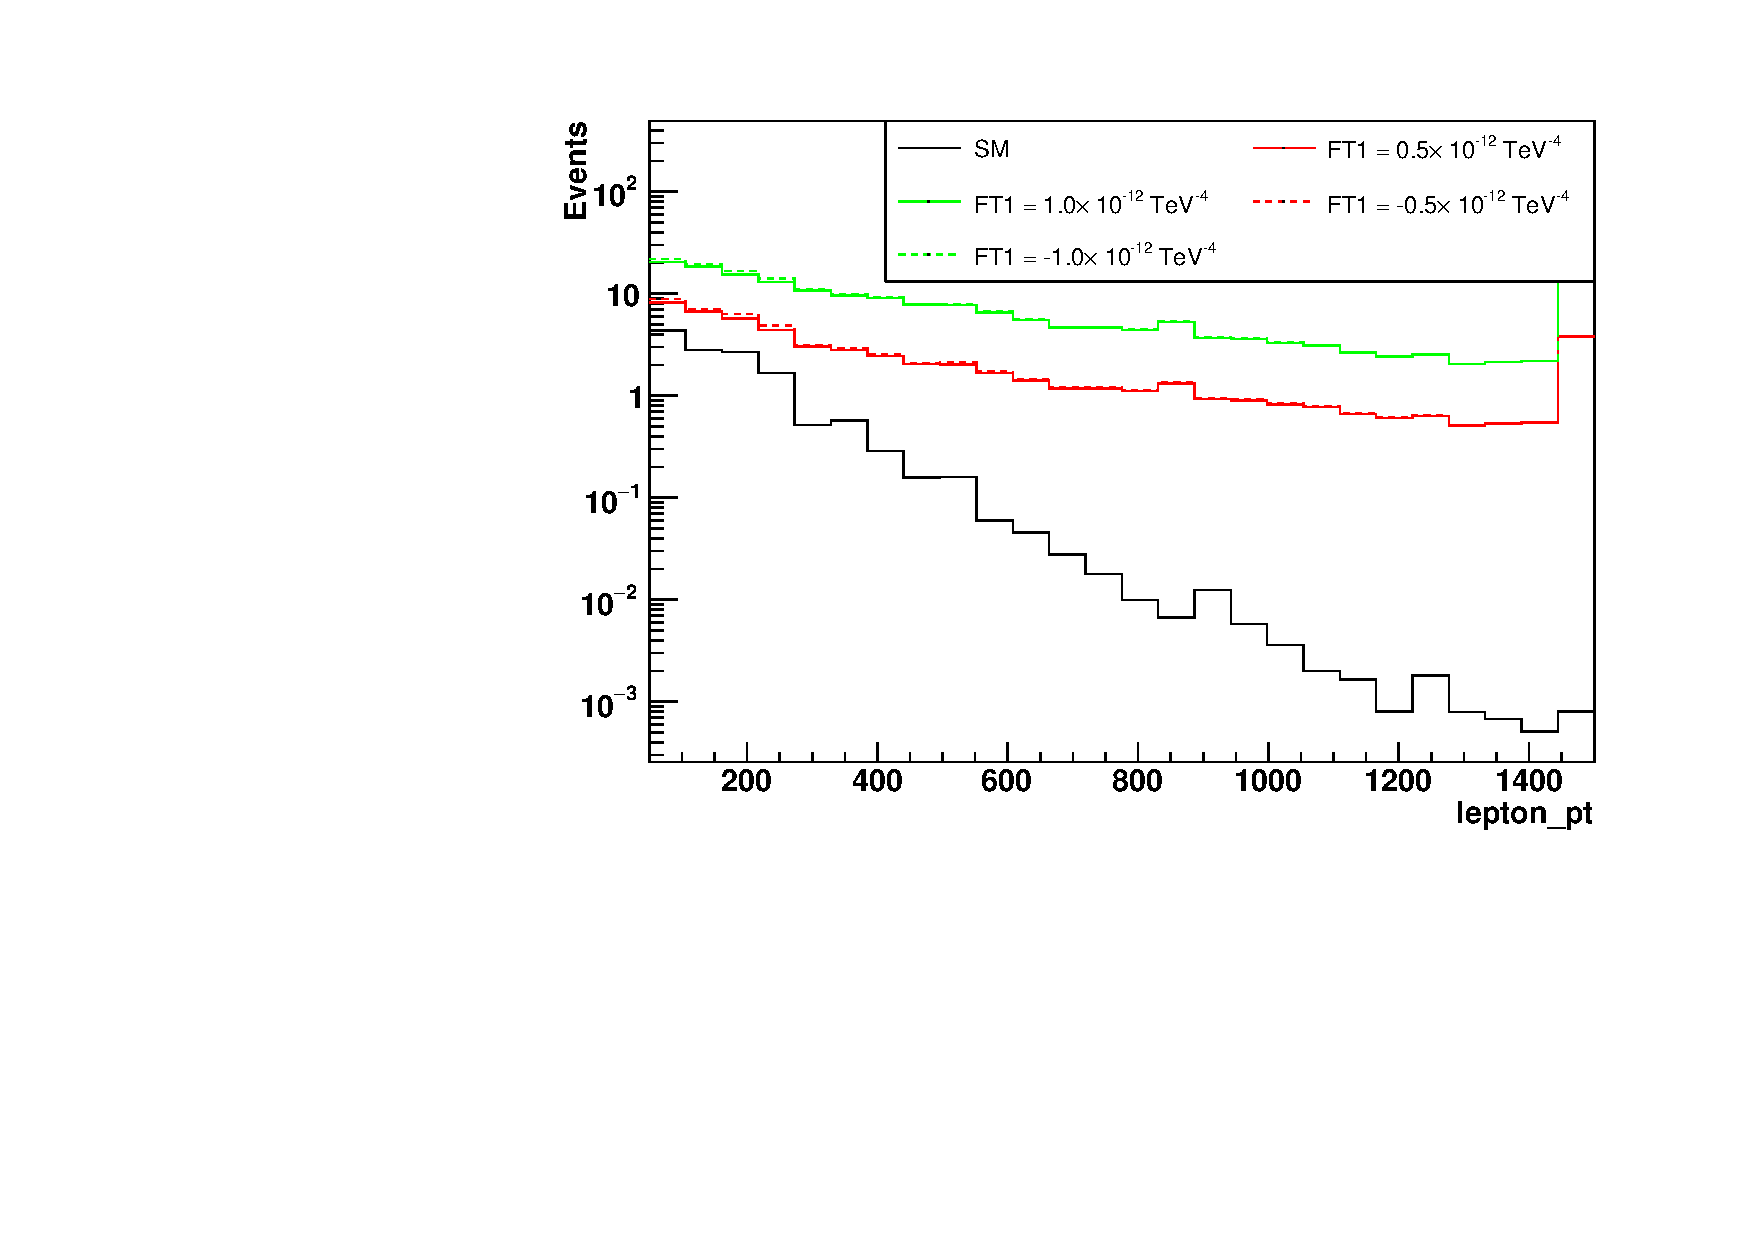
\includegraphics[width=0.45\textwidth]{Plots/aQGC_kinematics/lepton_pt_FT1_log.pdf}\\				
    \caption{}
  \end{center}
\end{figure}

\begin{figure}[h]
  \begin{center}
	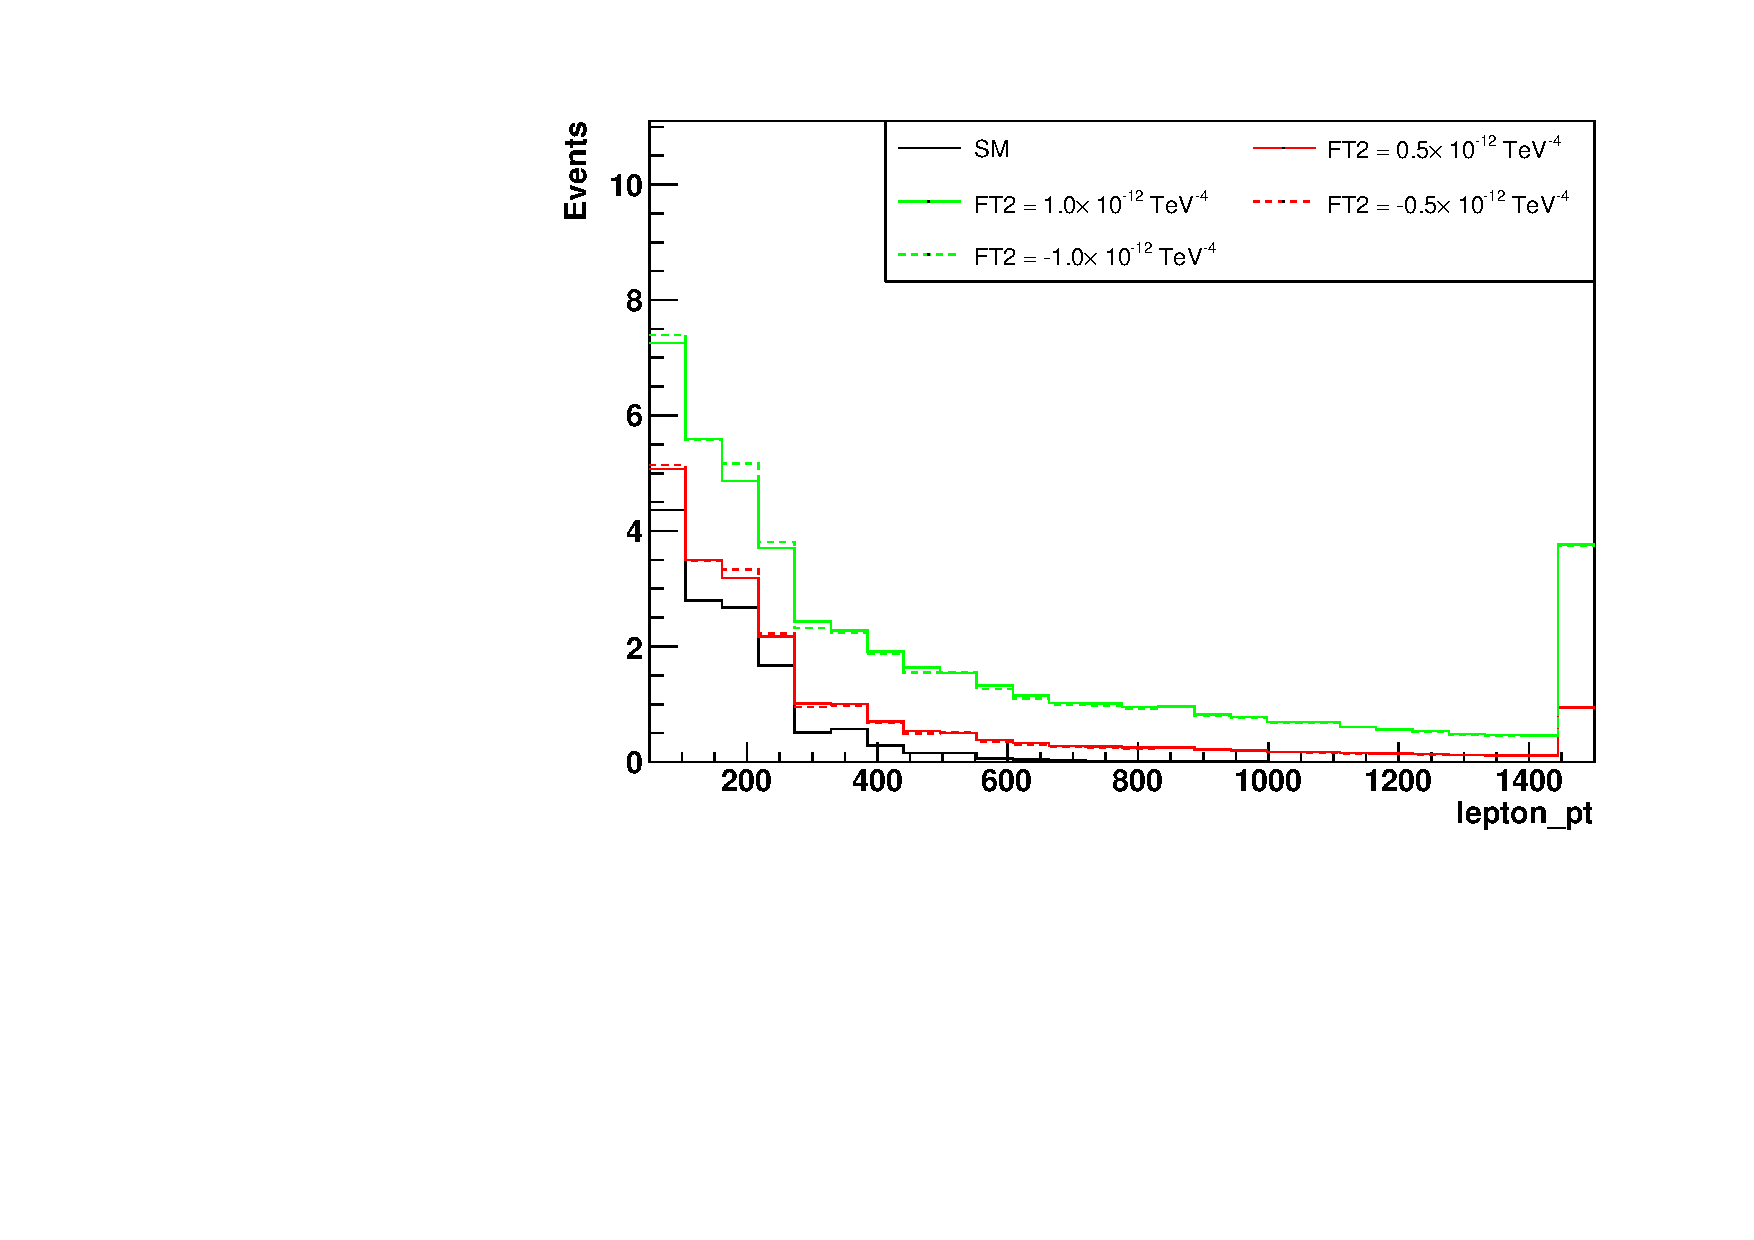
\includegraphics[width=0.45\textwidth]{Plots/aQGC_kinematics/lepton_pt_FT2.pdf}%	
	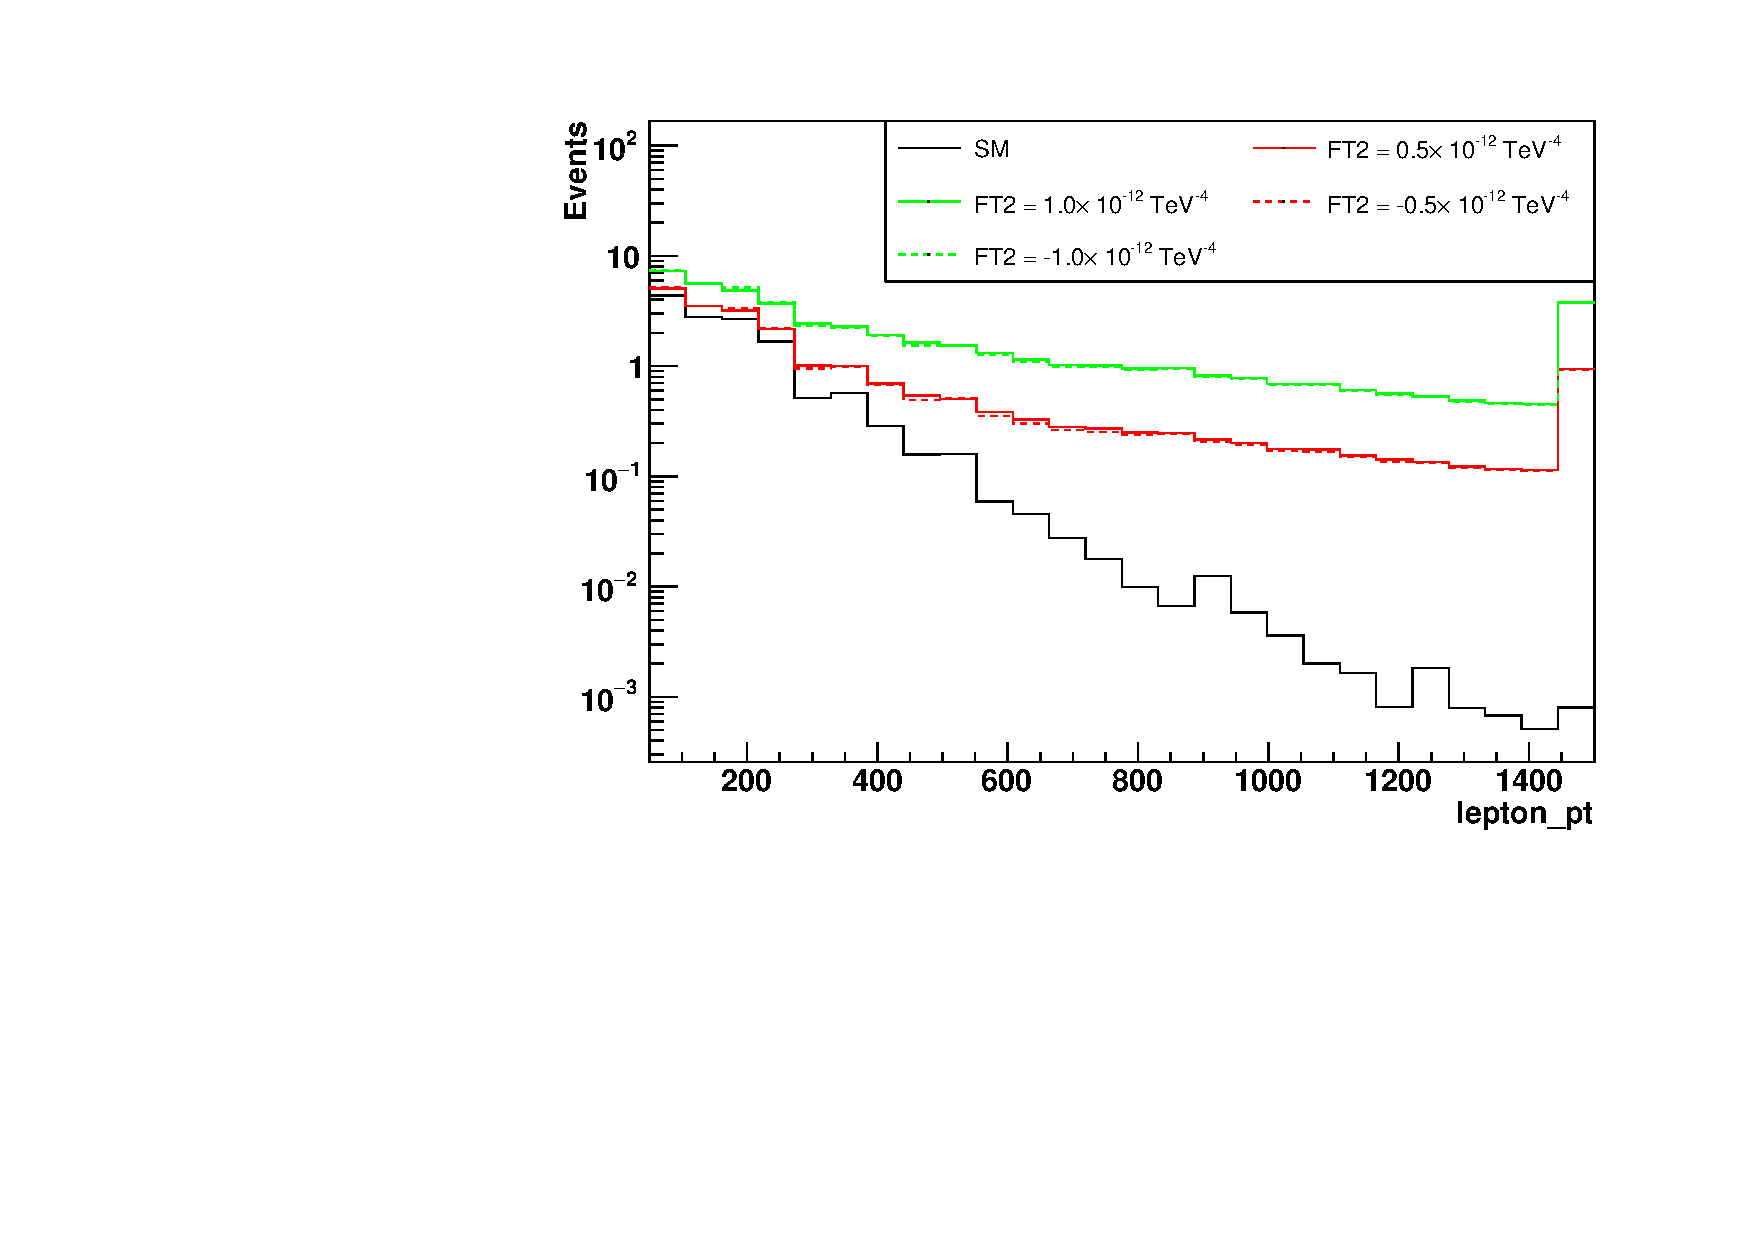
\includegraphics[width=0.45\textwidth]{Plots/aQGC_kinematics/lepton_pt_FT2_log.pdf}\\				
    \caption{}
  \end{center}
\end{figure}

\begin{figure}[h]
  \begin{center}
	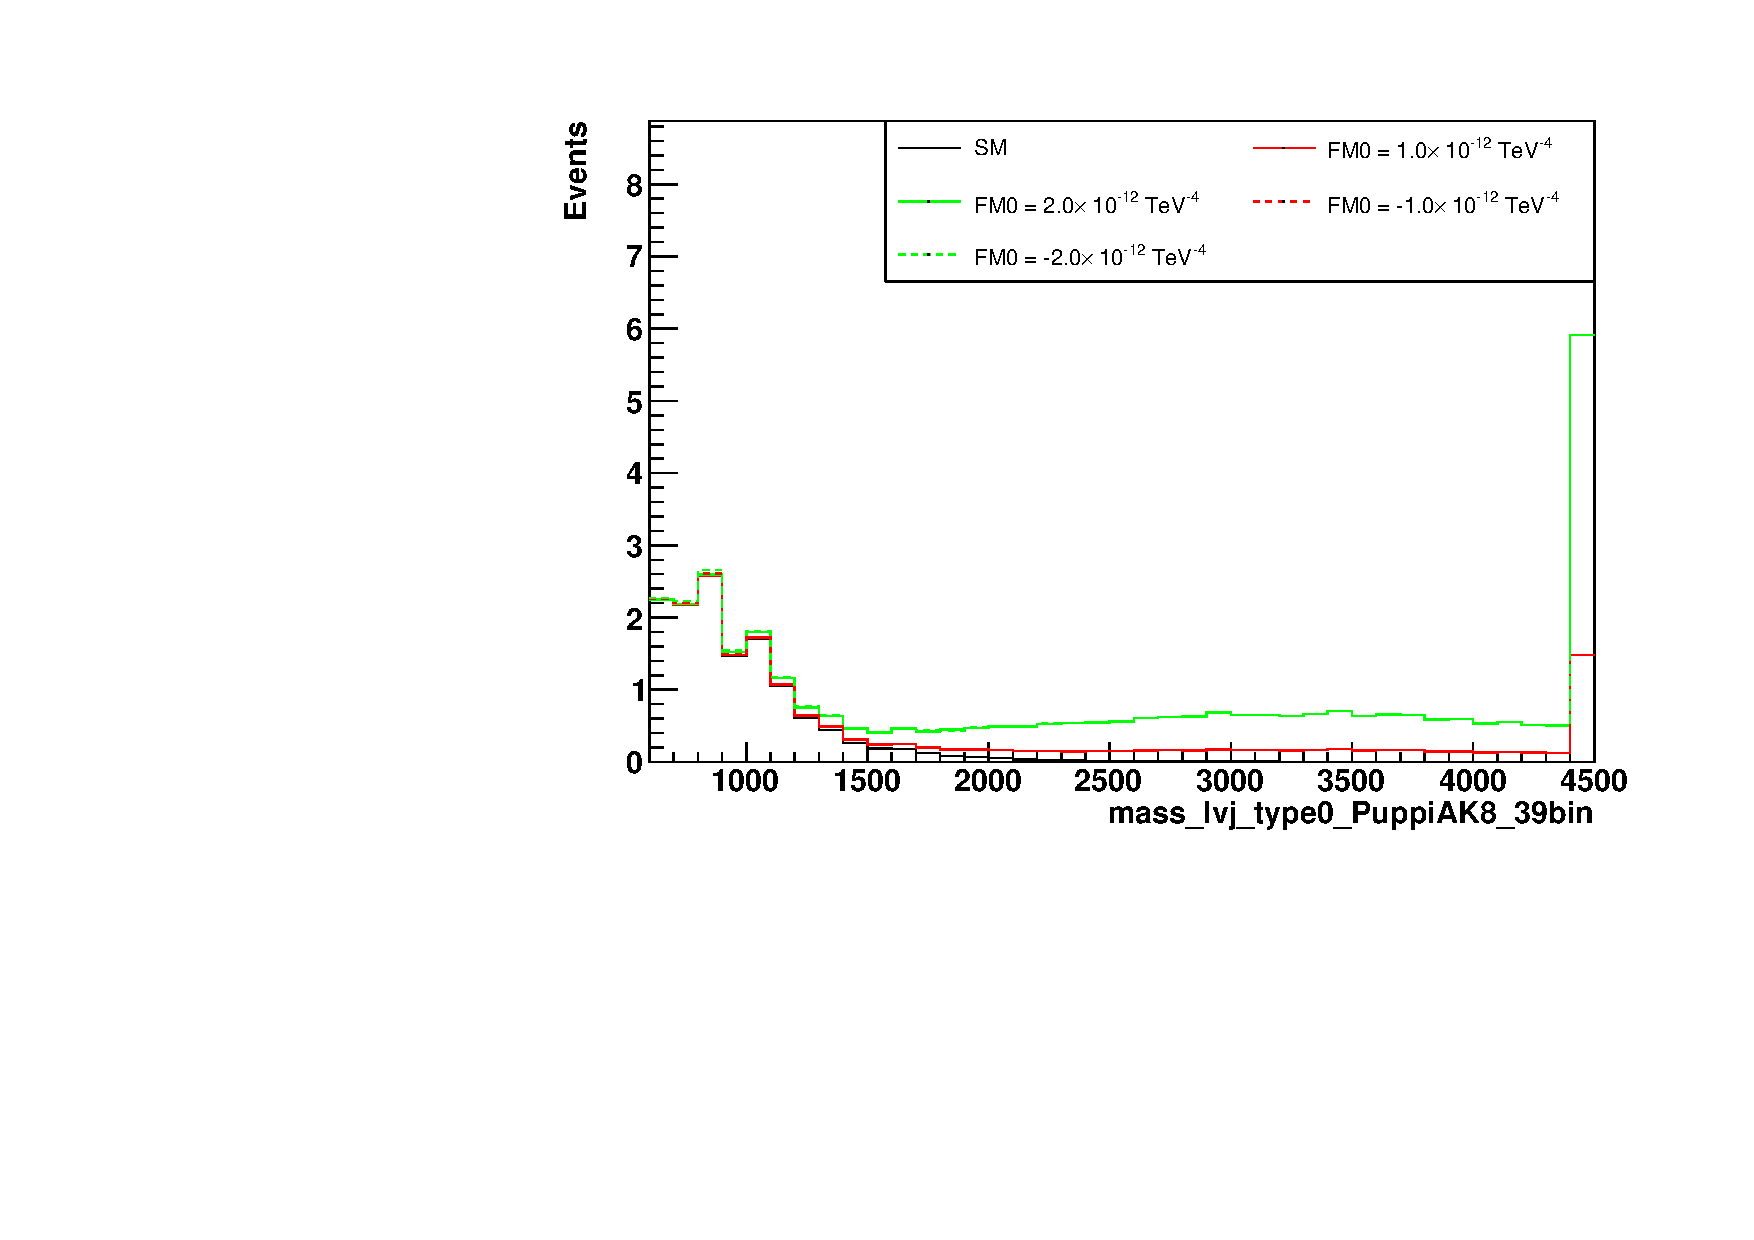
\includegraphics[width=0.45\textwidth]{Plots/aQGC_kinematics/mass_lvj_type0_PuppiAK8_39bin_FM0.pdf}%		
	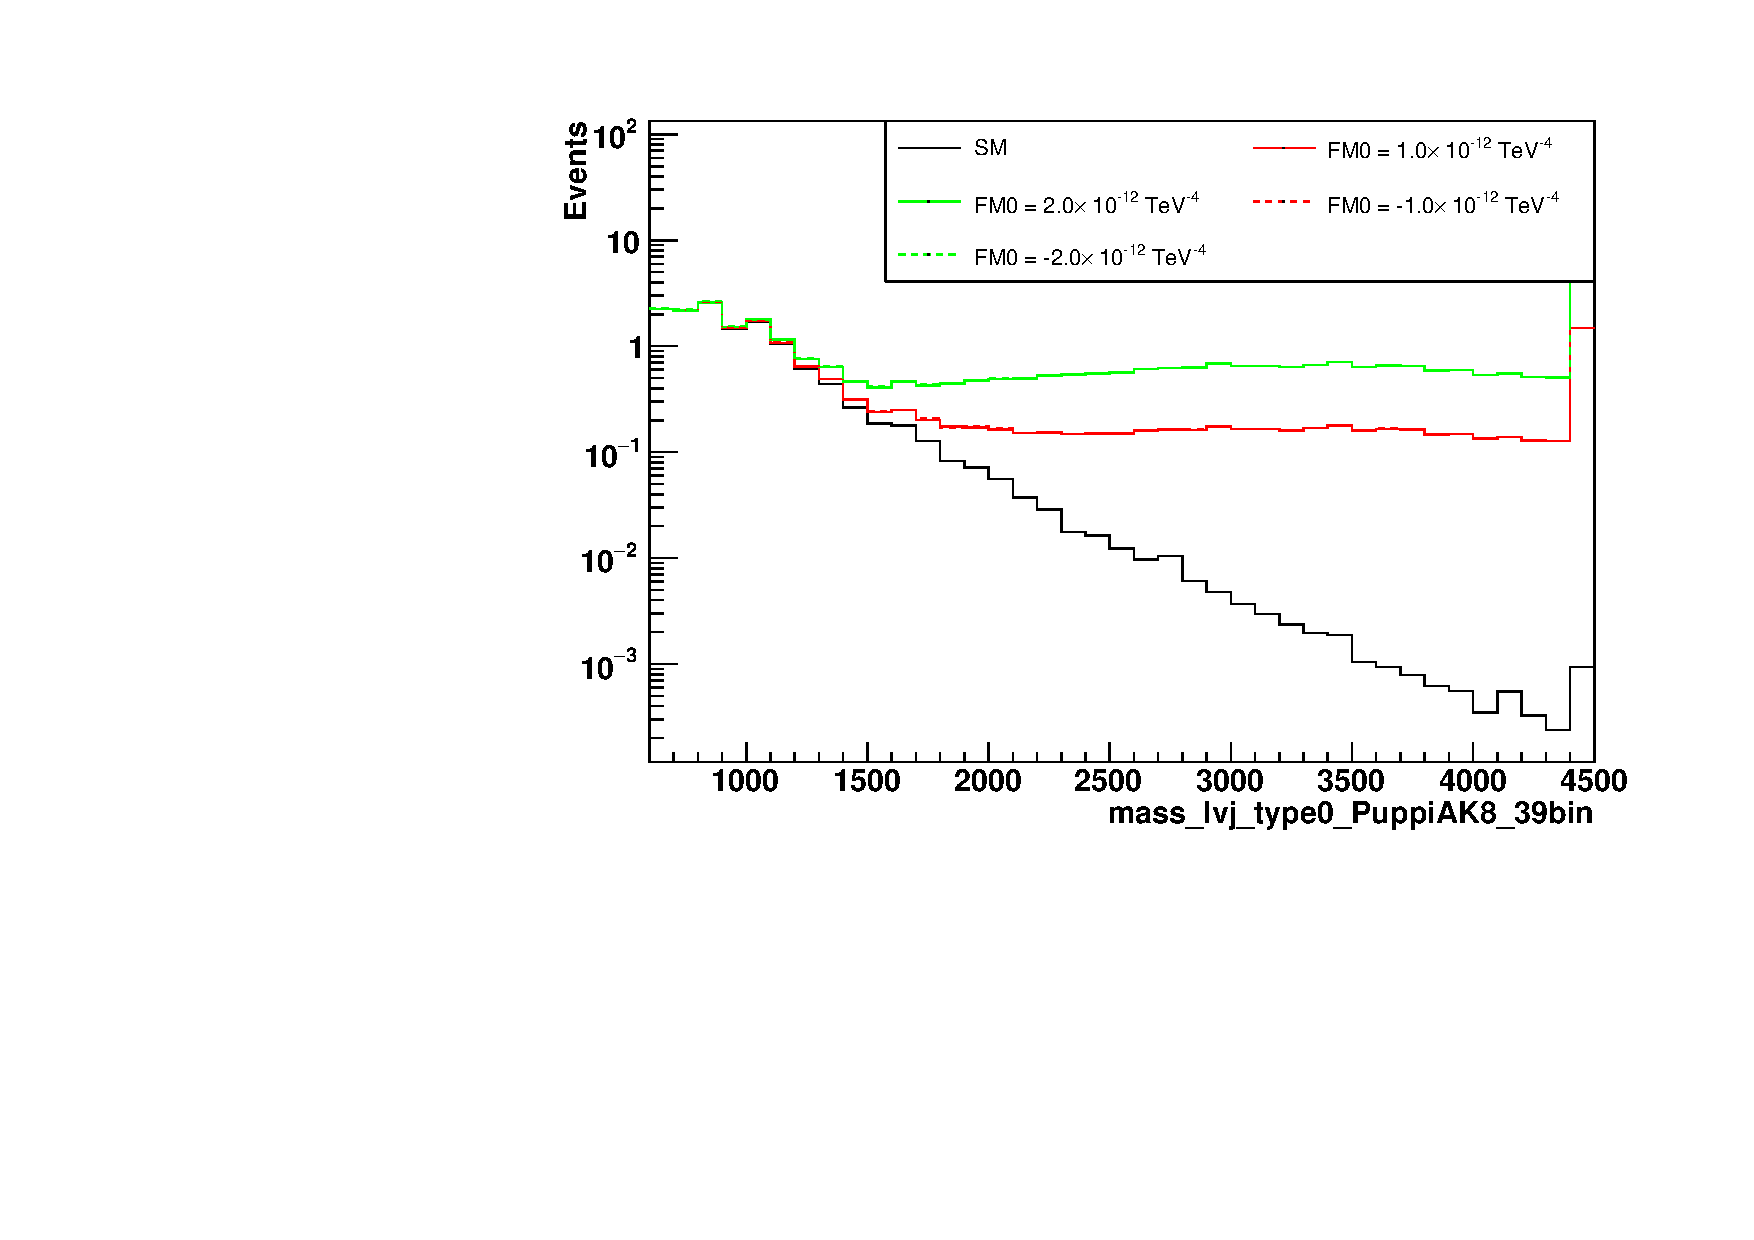
\includegraphics[width=0.45\textwidth]{Plots/aQGC_kinematics/mass_lvj_type0_PuppiAK8_39bin_FM0_log.pdf}\\	
    \caption{}
  \end{center}
\end{figure}

\begin{figure}[h]
  \begin{center}
	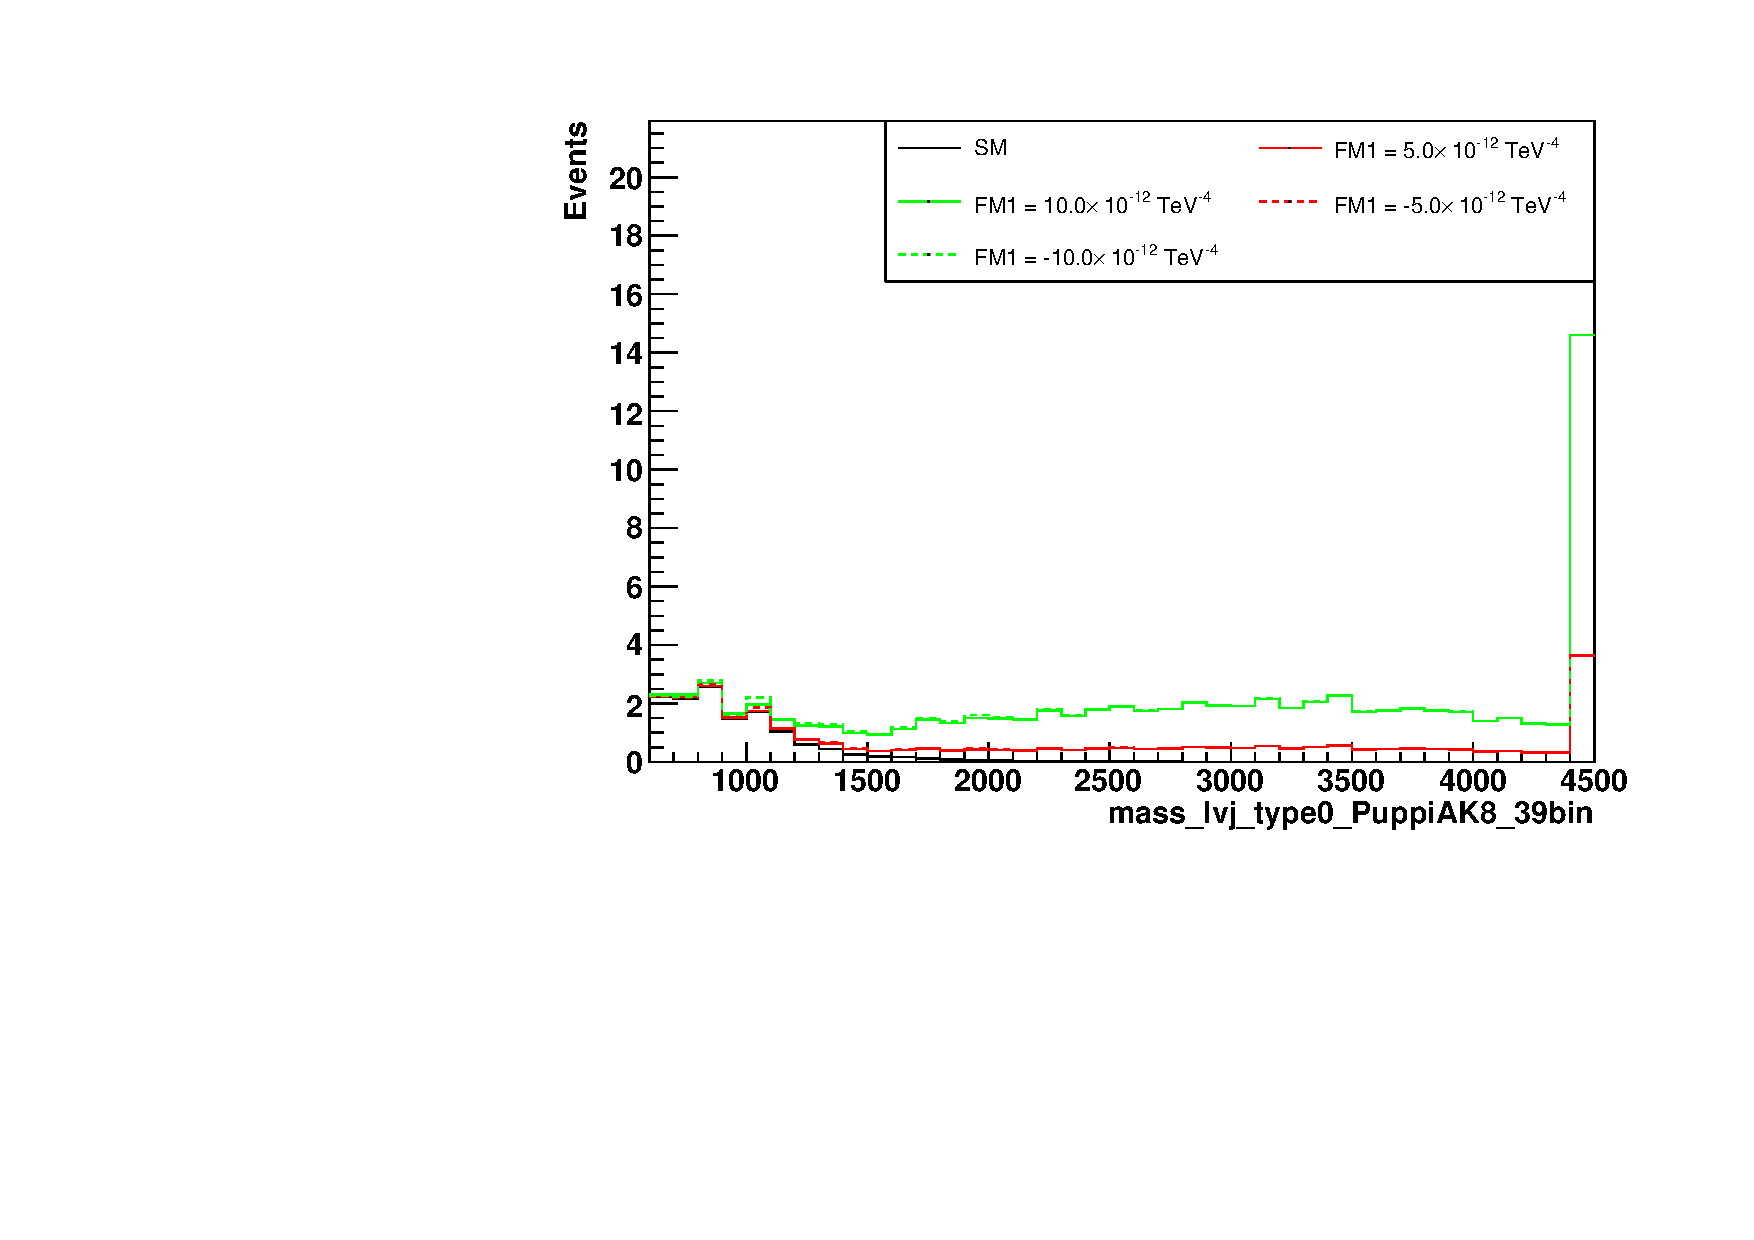
\includegraphics[width=0.45\textwidth]{Plots/aQGC_kinematics/mass_lvj_type0_PuppiAK8_39bin_FM1.pdf}%		
	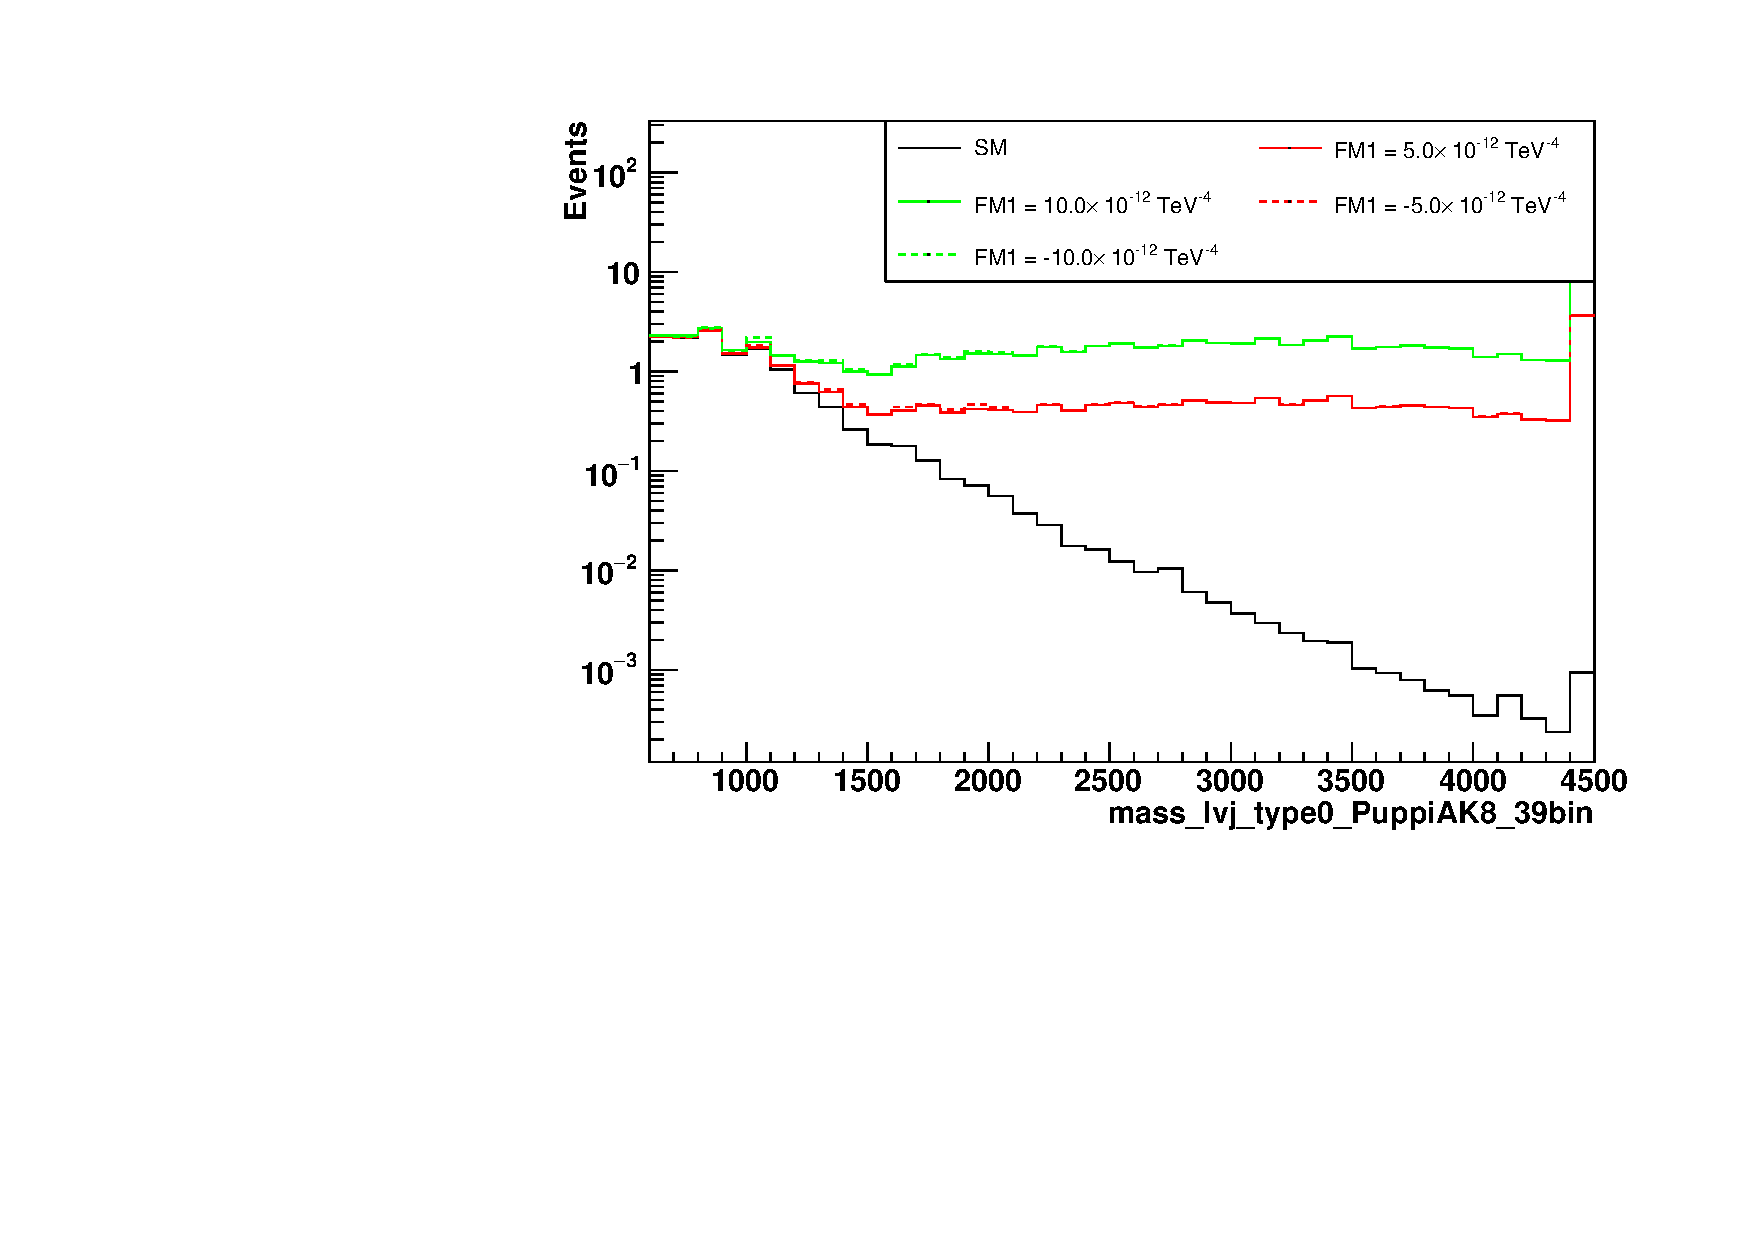
\includegraphics[width=0.45\textwidth]{Plots/aQGC_kinematics/mass_lvj_type0_PuppiAK8_39bin_FM1_log.pdf}\\	
    \caption{}
  \end{center}
\end{figure}
\begin{figure}[h]
  \begin{center}
	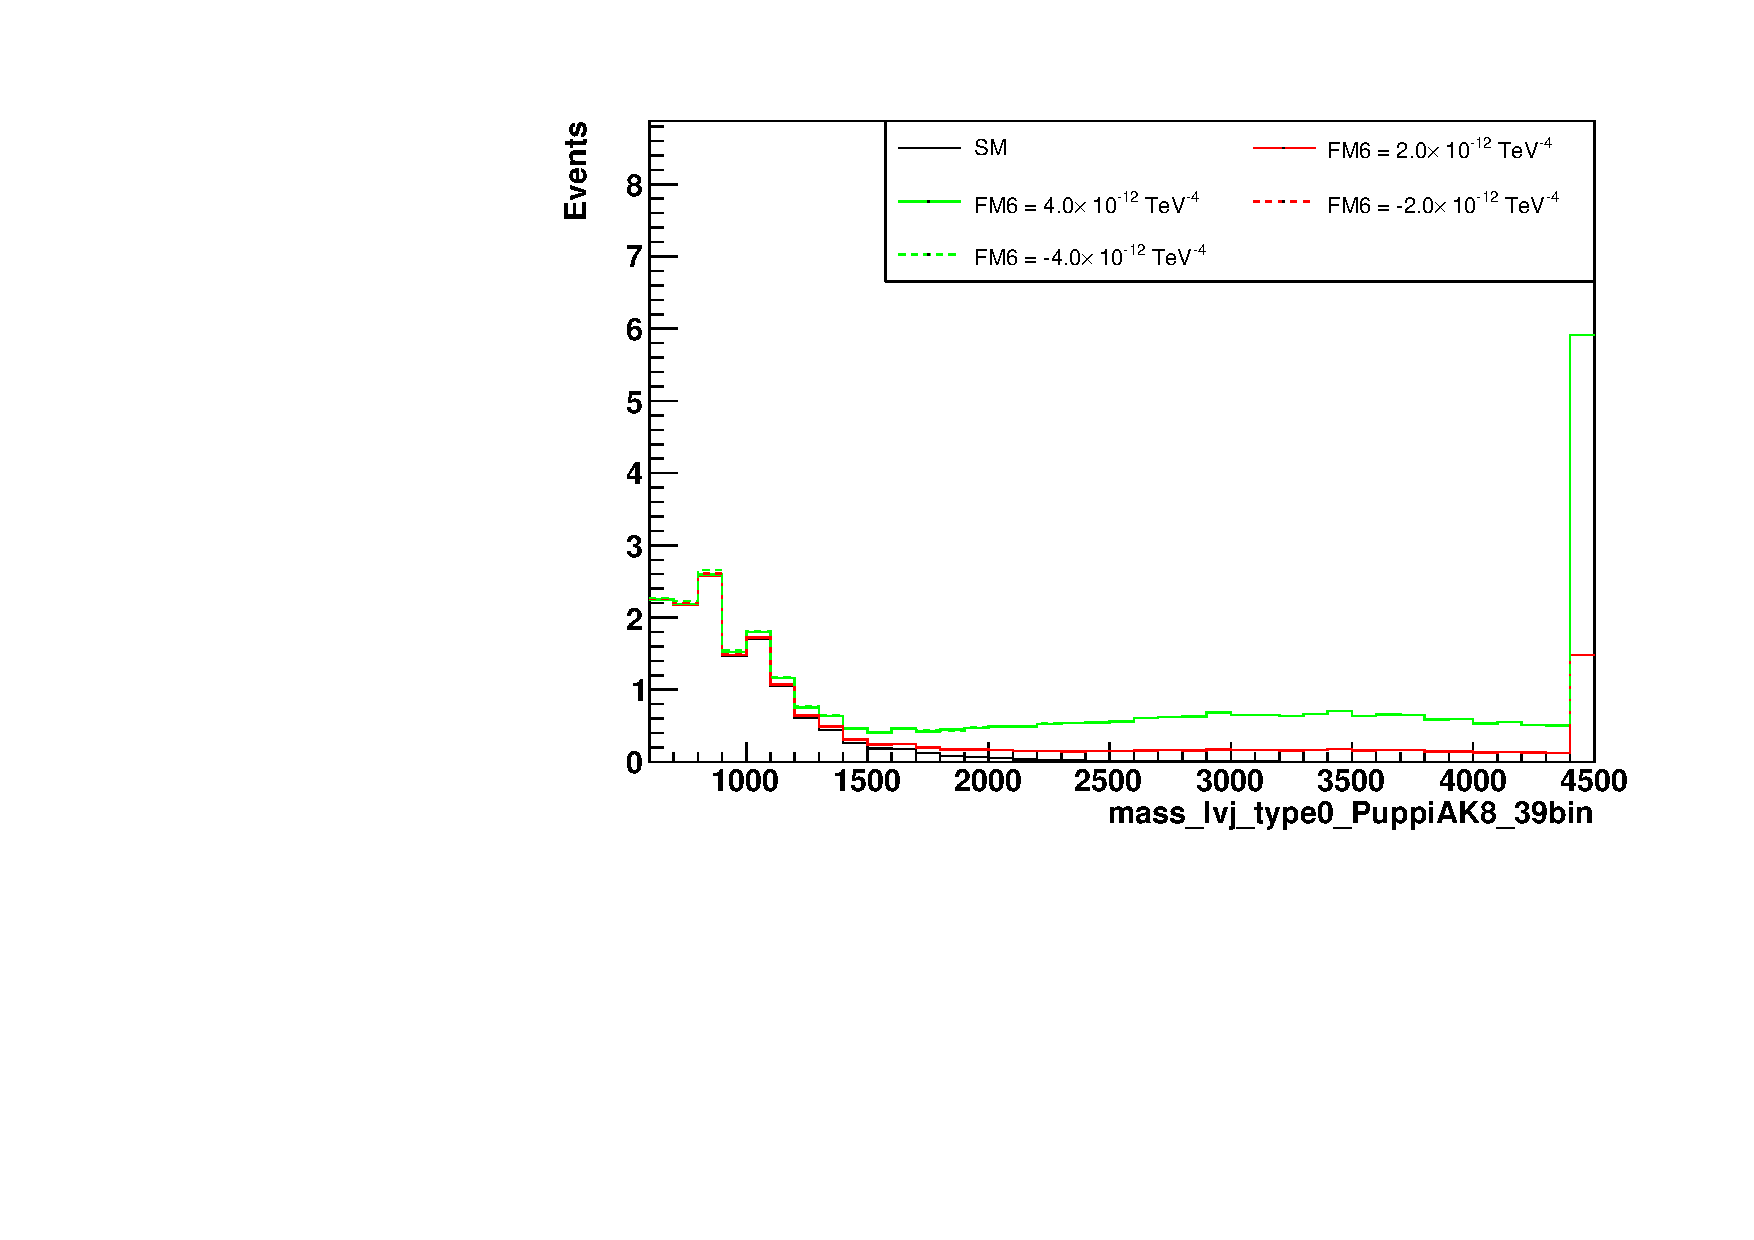
\includegraphics[width=0.45\textwidth]{Plots/aQGC_kinematics/mass_lvj_type0_PuppiAK8_39bin_FM6.pdf}%		
	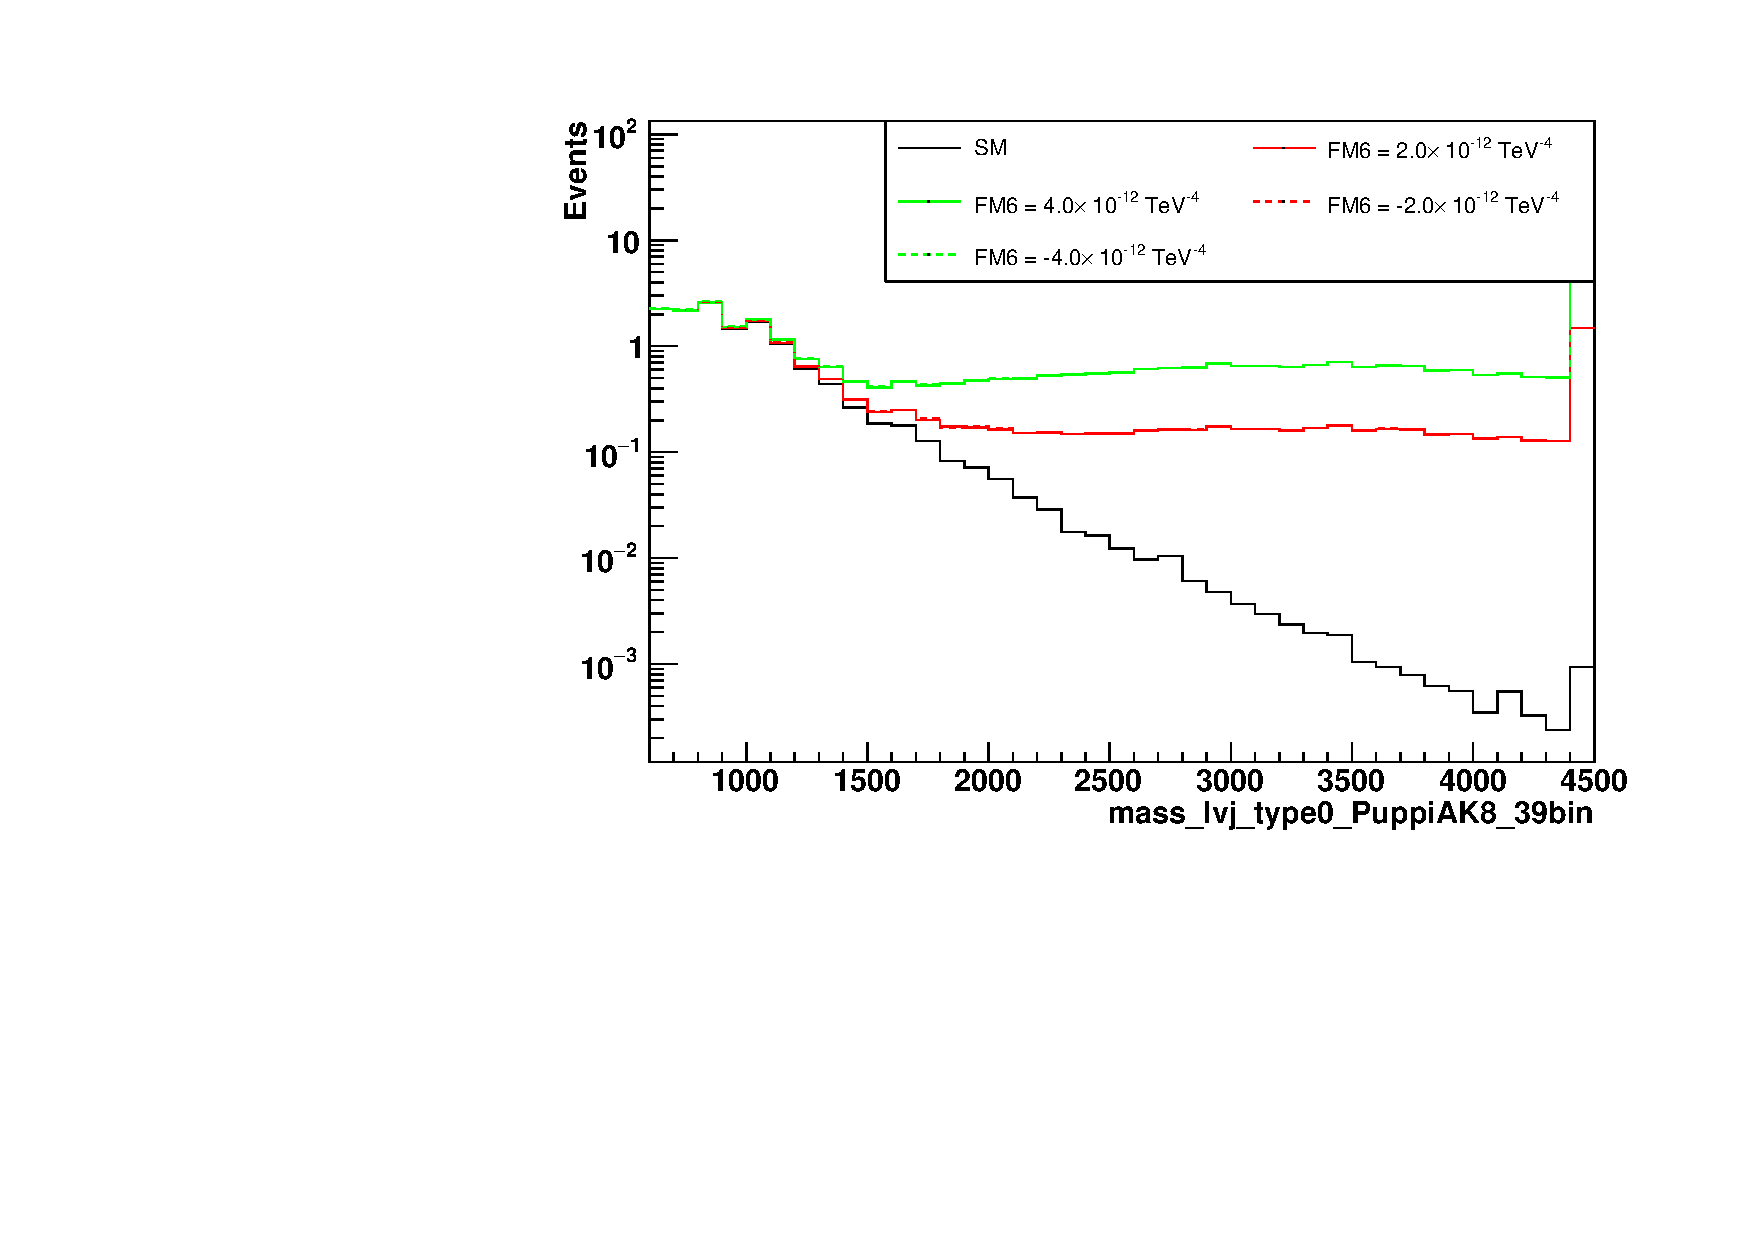
\includegraphics[width=0.45\textwidth]{Plots/aQGC_kinematics/mass_lvj_type0_PuppiAK8_39bin_FM6_log.pdf}\\	
    \caption{}
  \end{center}
\end{figure}
\begin{figure}[h]
  \begin{center}
	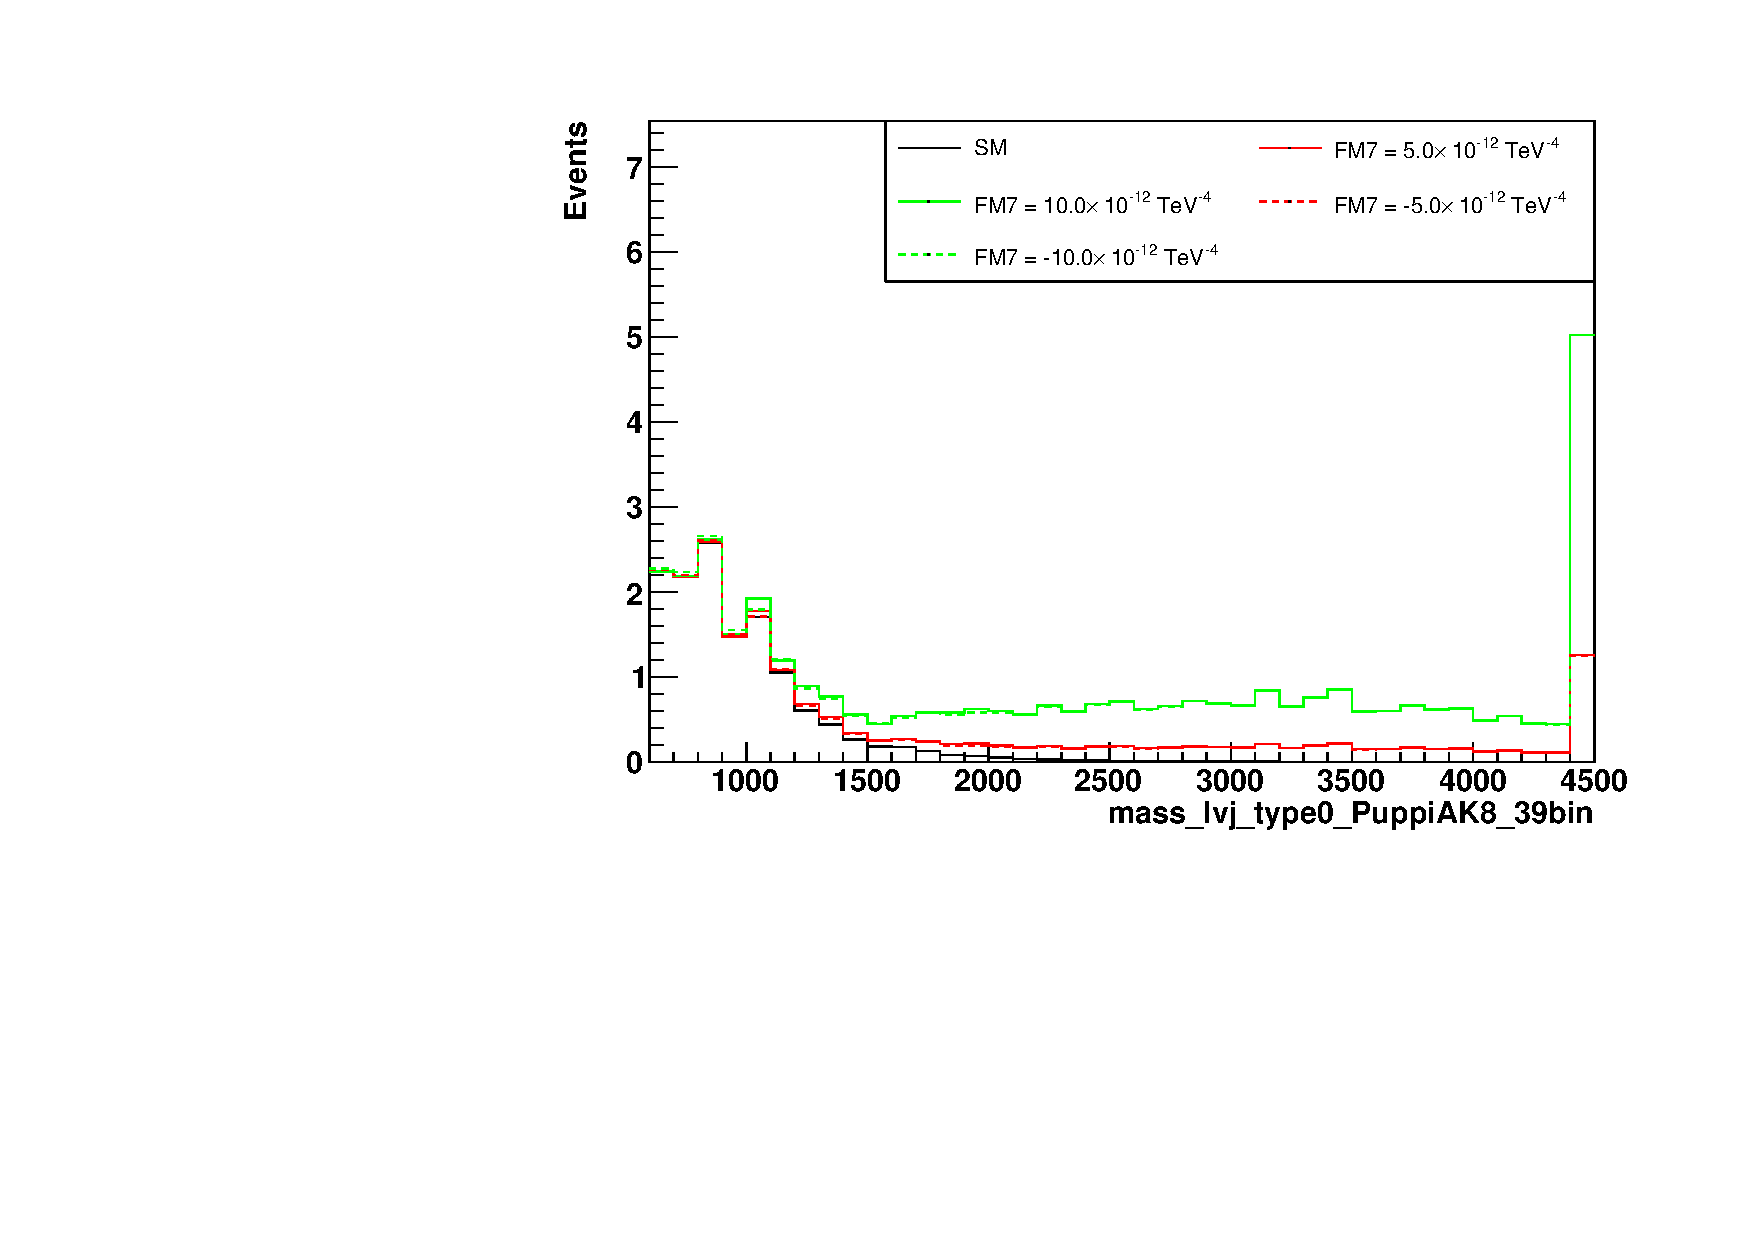
\includegraphics[width=0.45\textwidth]{Plots/aQGC_kinematics/mass_lvj_type0_PuppiAK8_39bin_FM7.pdf}%		
	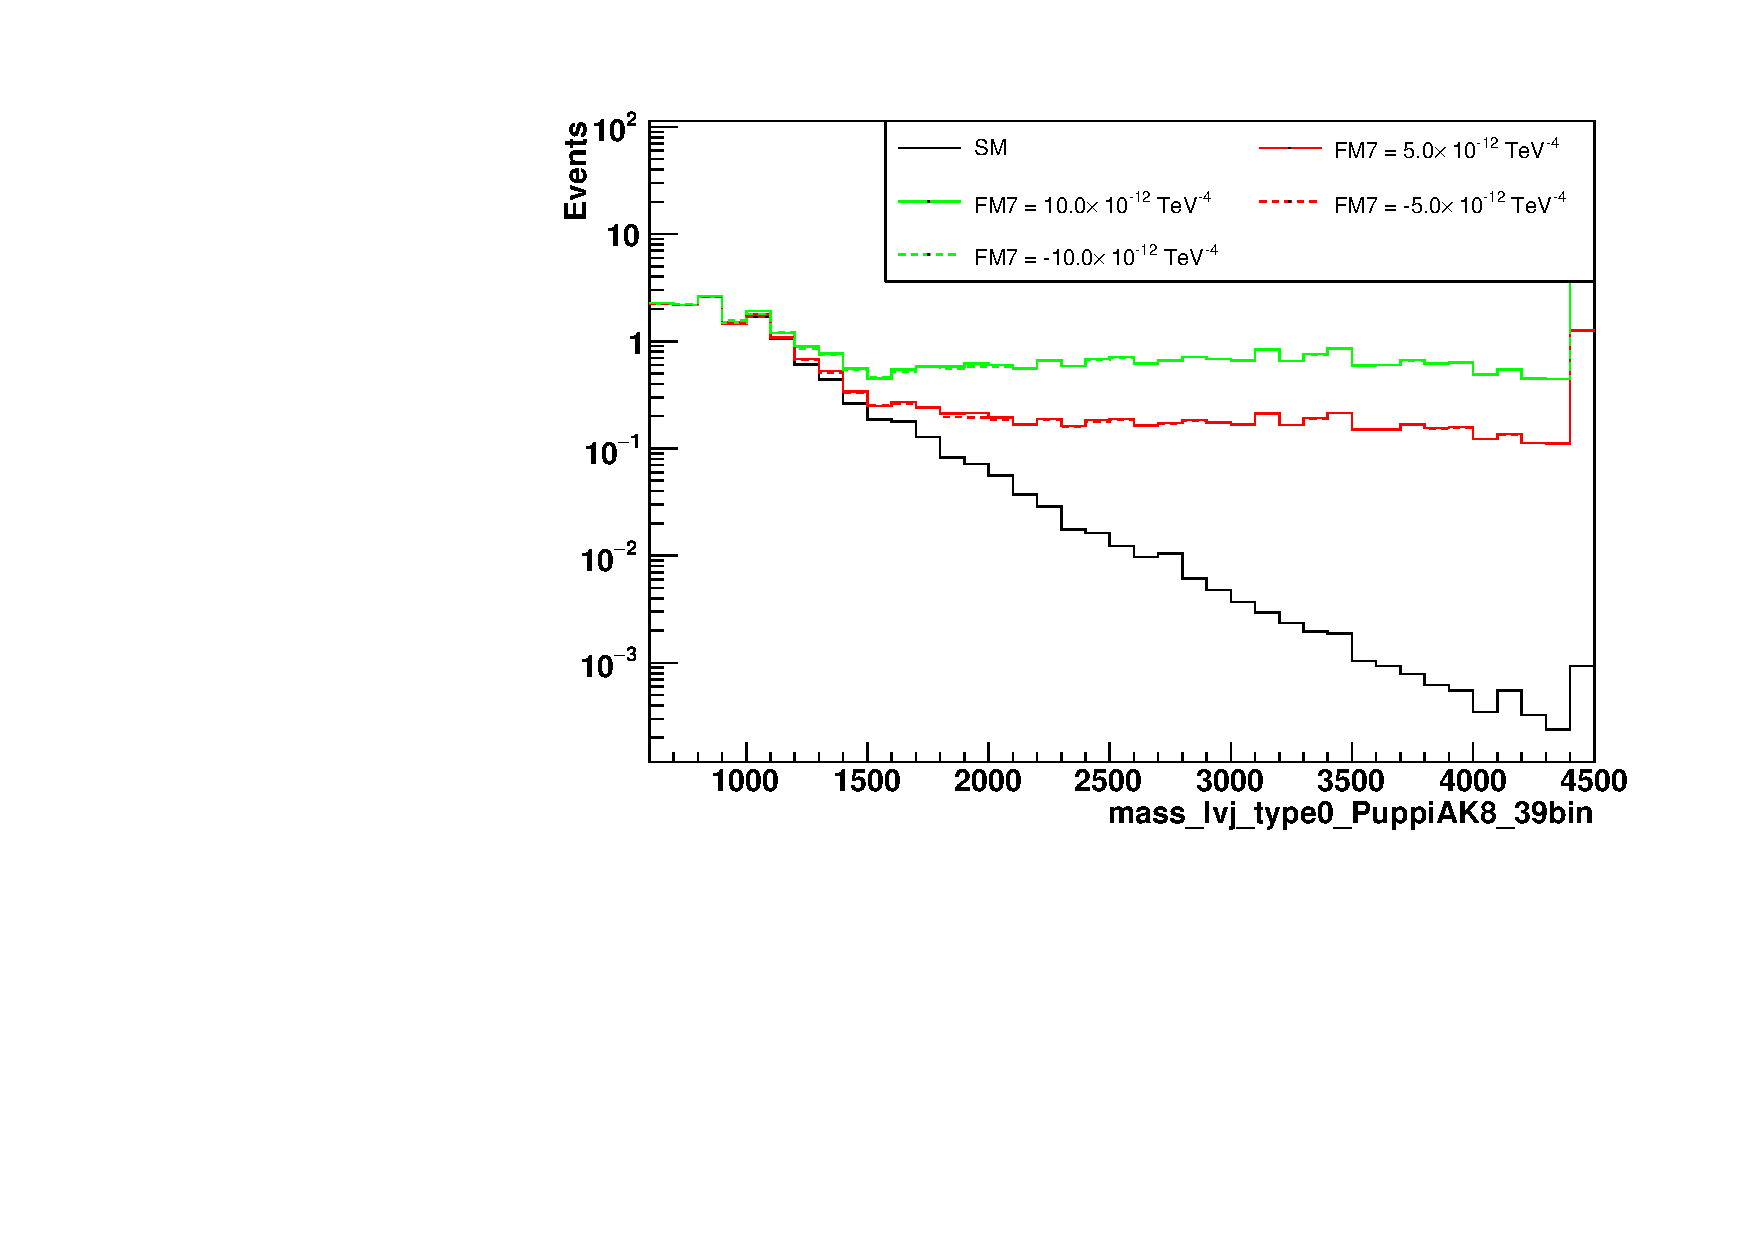
\includegraphics[width=0.45\textwidth]{Plots/aQGC_kinematics/mass_lvj_type0_PuppiAK8_39bin_FM7_log.pdf}\\	
    \caption{}
  \end{center}
\end{figure}
\begin{figure}[h]
  \begin{center}
	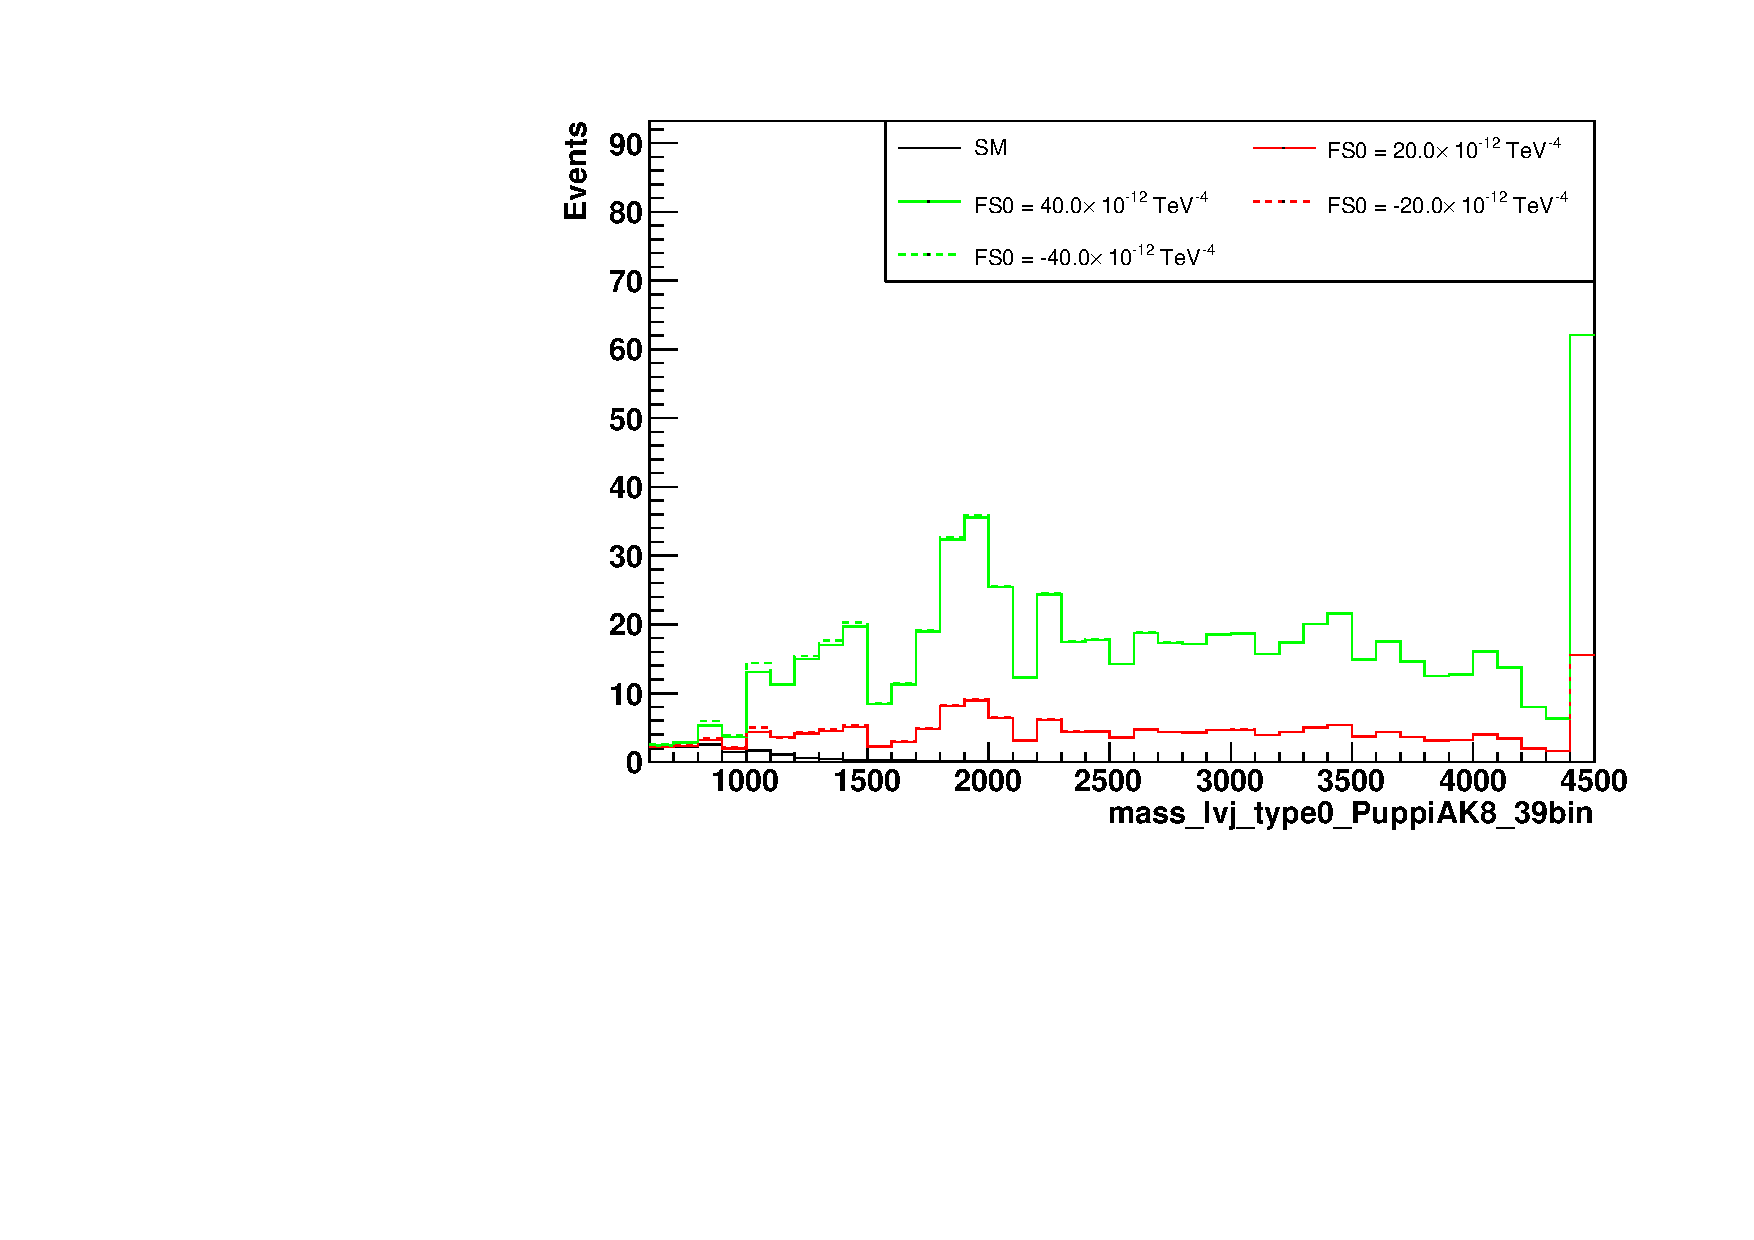
\includegraphics[width=0.45\textwidth]{Plots/aQGC_kinematics/mass_lvj_type0_PuppiAK8_39bin_FS0.pdf}%		
	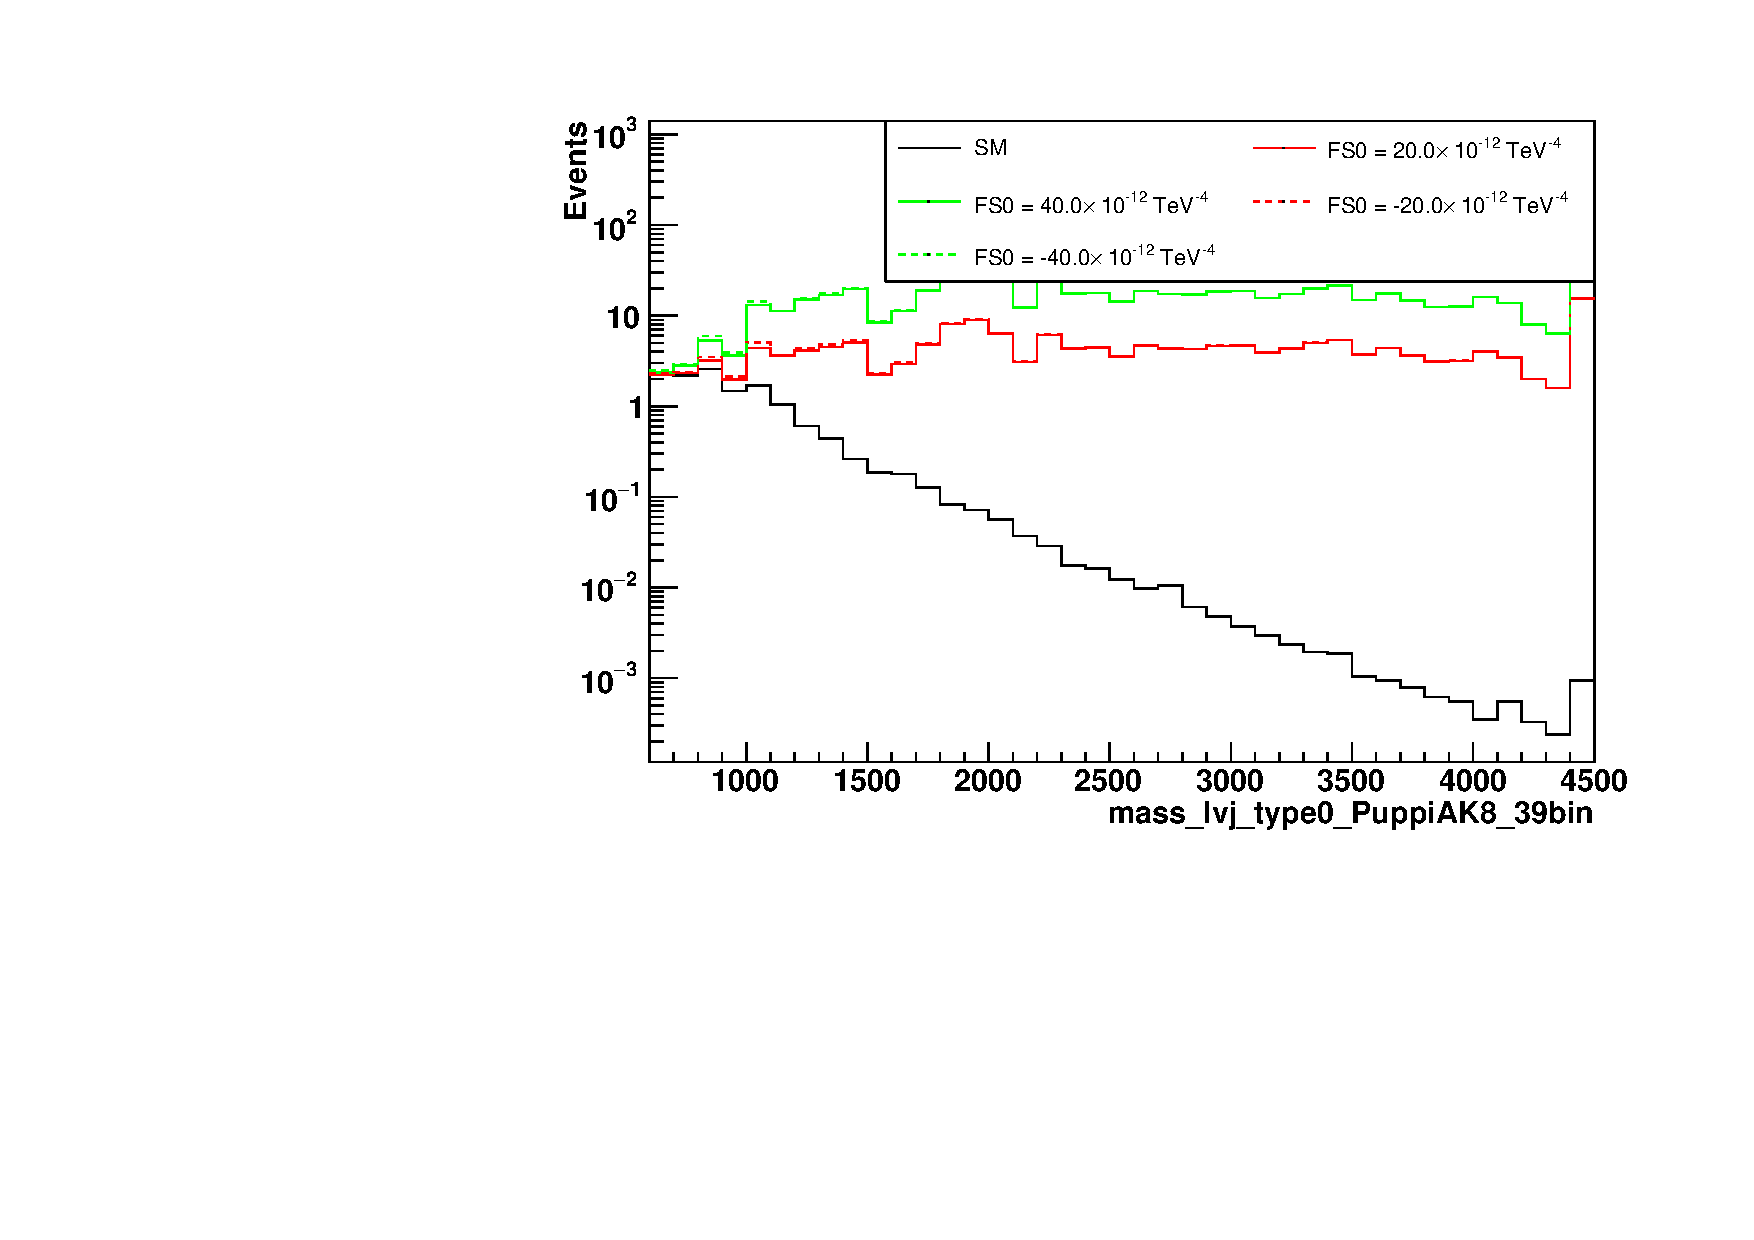
\includegraphics[width=0.45\textwidth]{Plots/aQGC_kinematics/mass_lvj_type0_PuppiAK8_39bin_FS0_log.pdf}\\	
    \caption{}
  \end{center}
\end{figure}
\begin{figure}[h]
  \begin{center}
	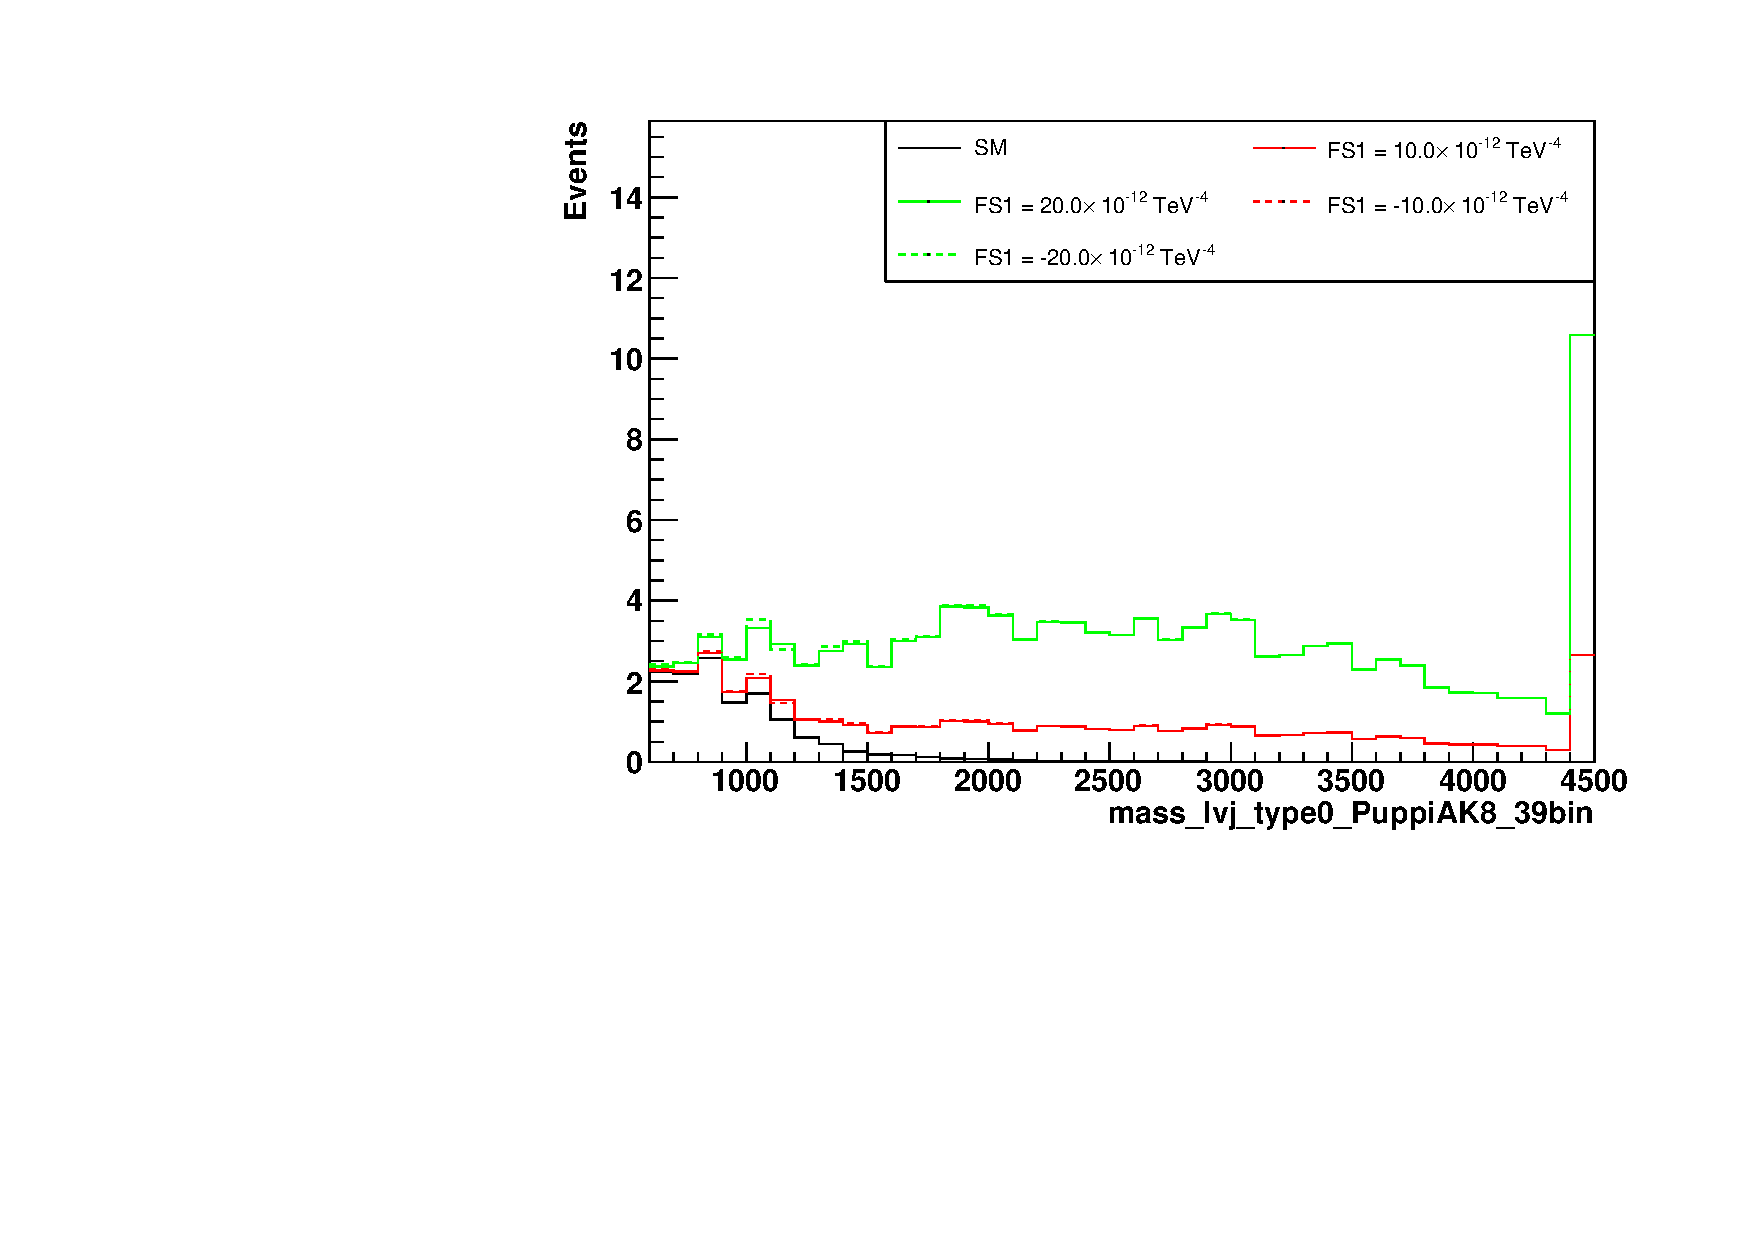
\includegraphics[width=0.45\textwidth]{Plots/aQGC_kinematics/mass_lvj_type0_PuppiAK8_39bin_FS1.pdf}%		
	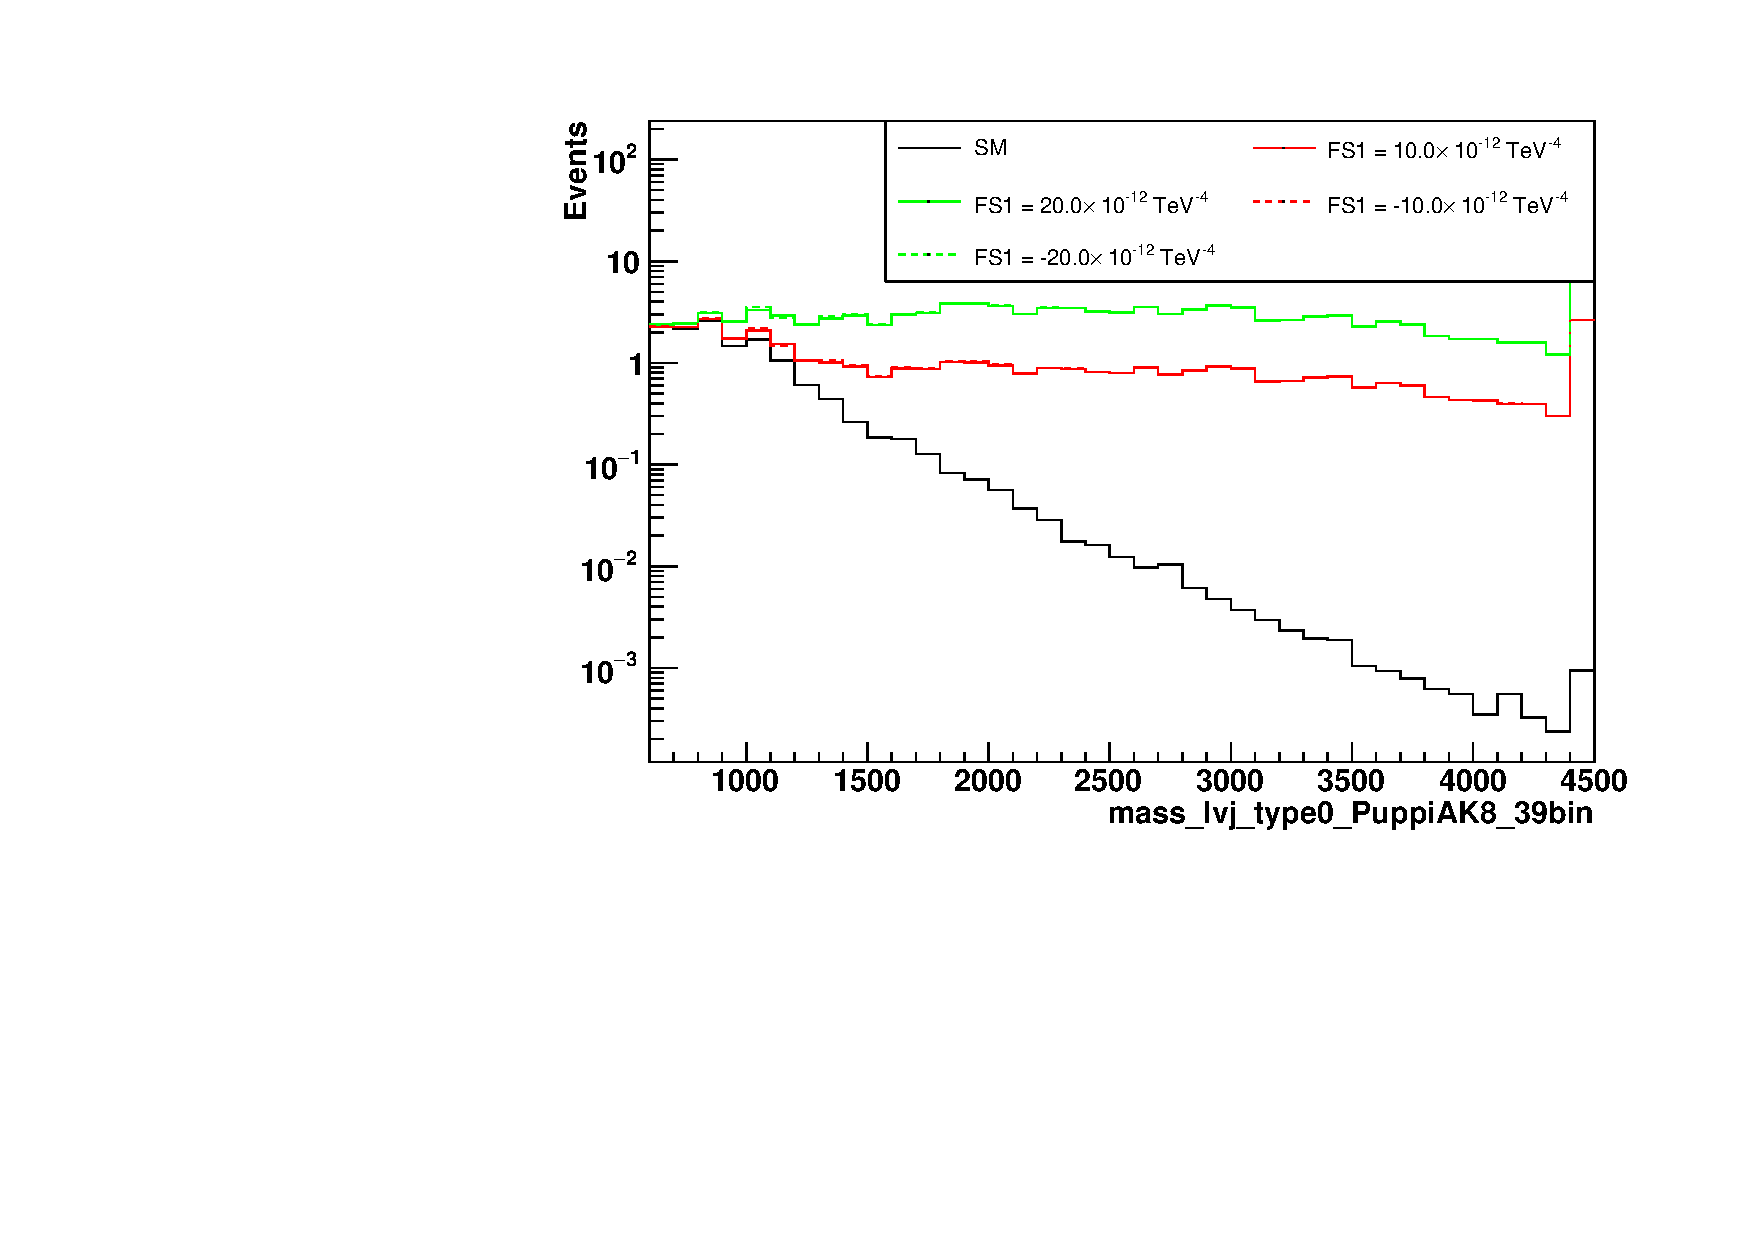
\includegraphics[width=0.45\textwidth]{Plots/aQGC_kinematics/mass_lvj_type0_PuppiAK8_39bin_FS1_log.pdf}\\	
    \caption{}
  \end{center}
\end{figure}
\begin{figure}[h]
  \begin{center}
	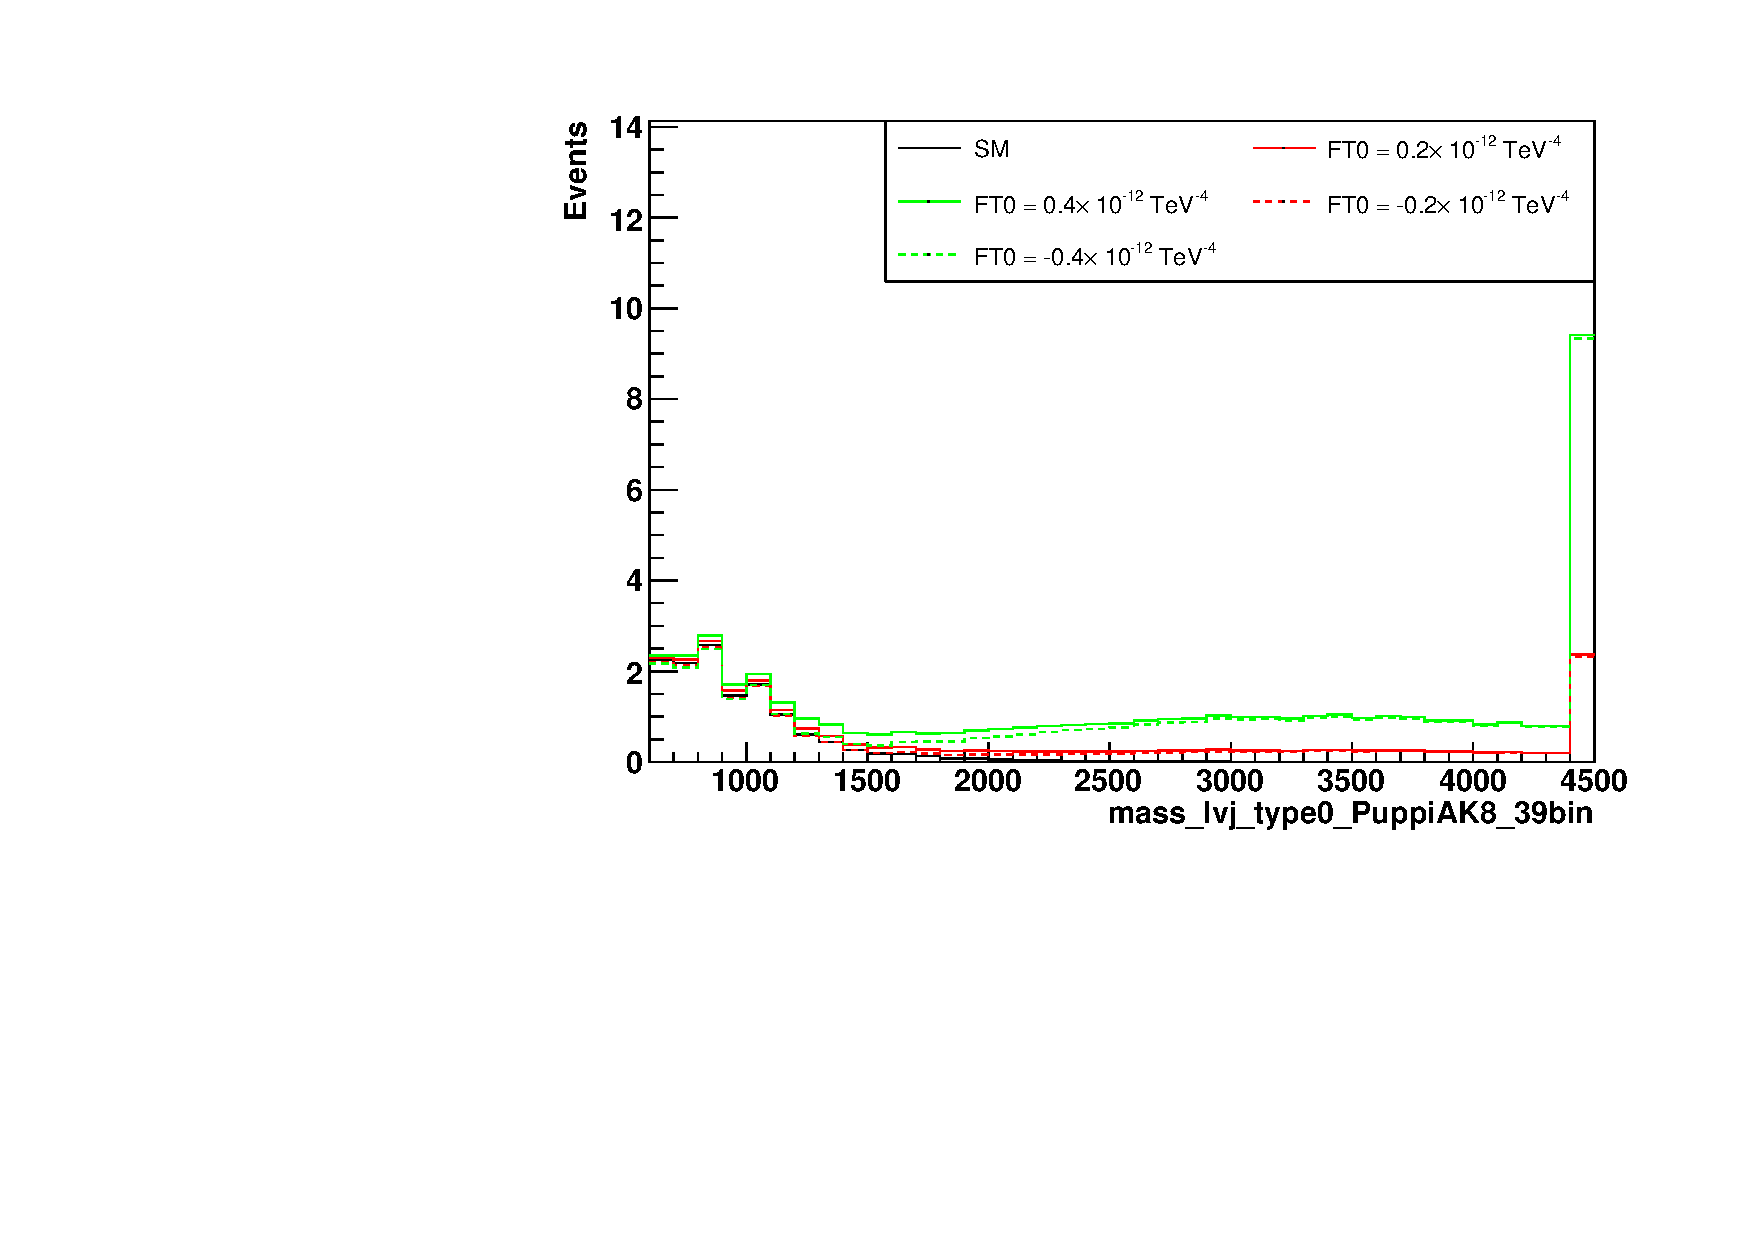
\includegraphics[width=0.45\textwidth]{Plots/aQGC_kinematics/mass_lvj_type0_PuppiAK8_39bin_FT0.pdf}%		
	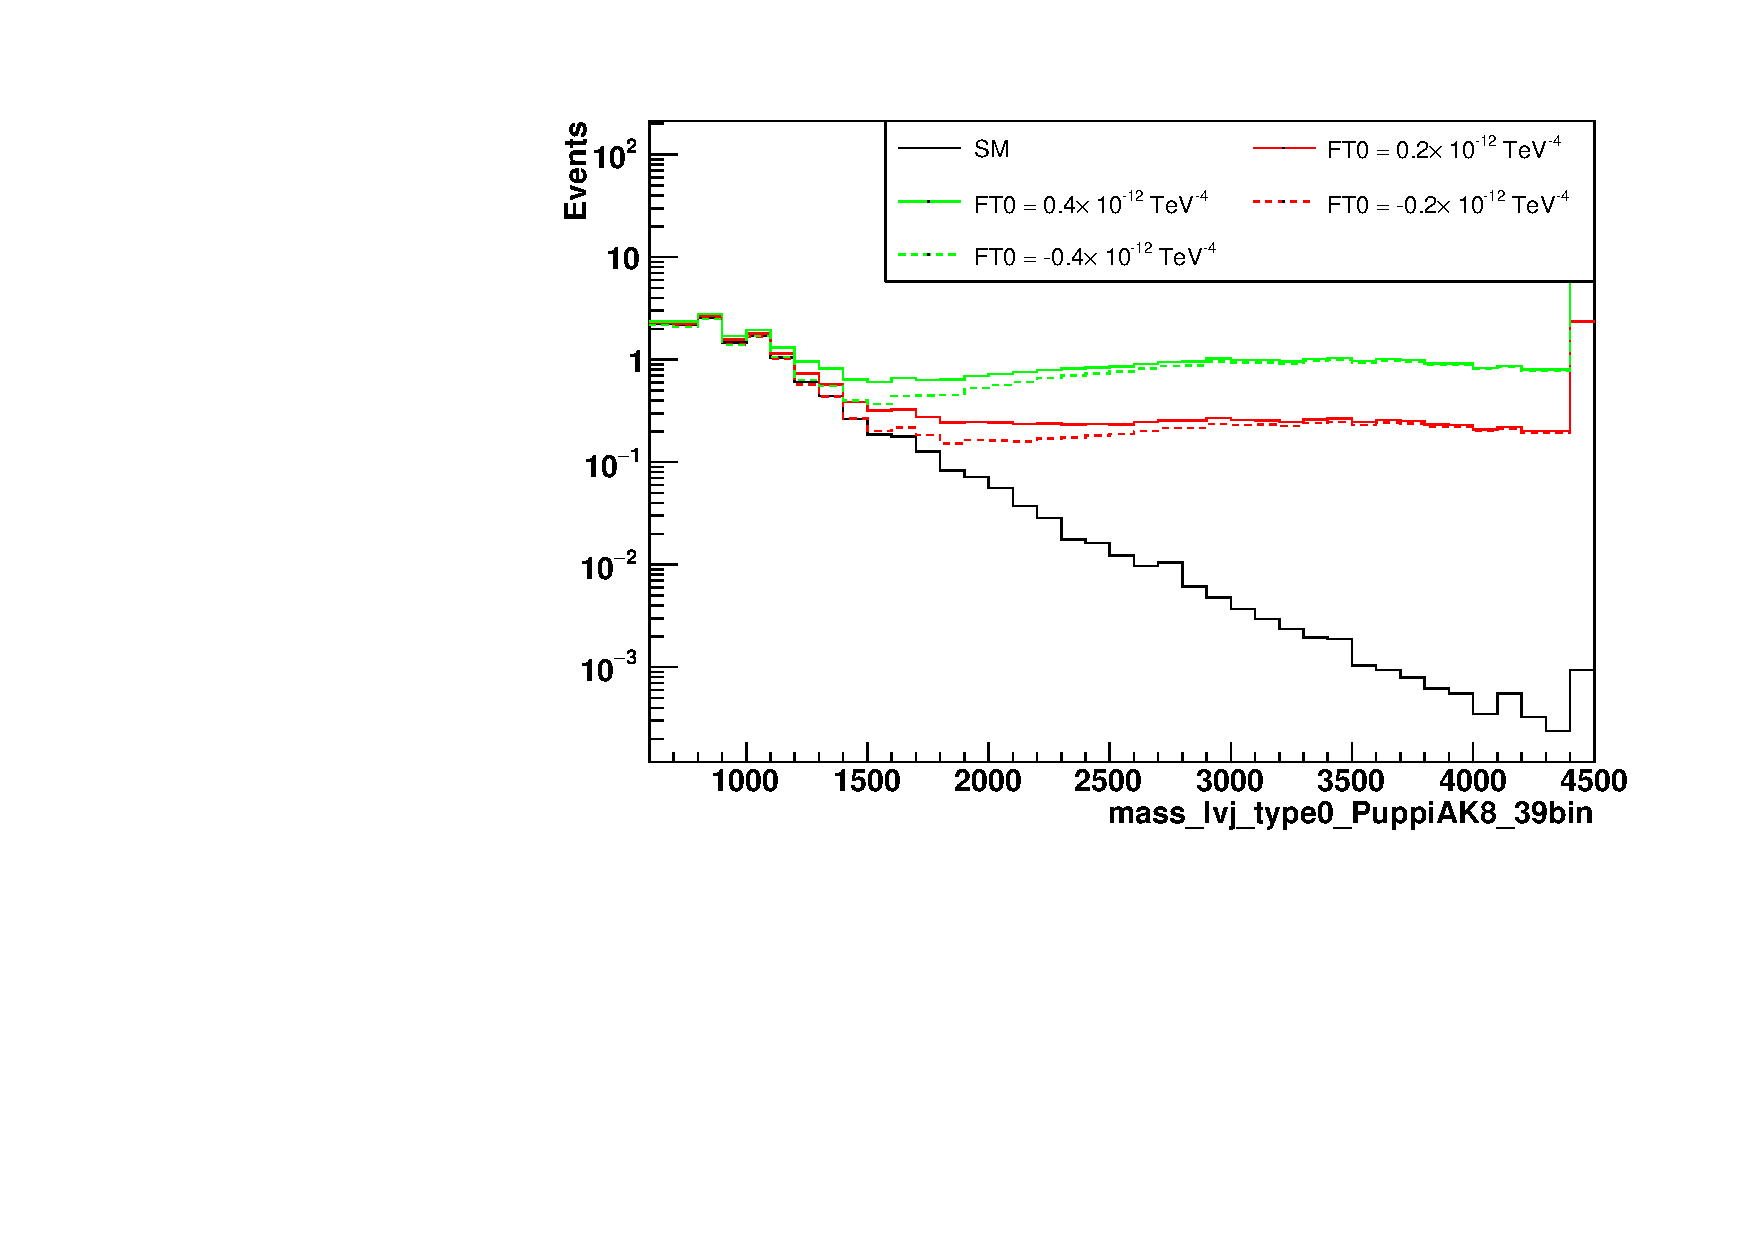
\includegraphics[width=0.45\textwidth]{Plots/aQGC_kinematics/mass_lvj_type0_PuppiAK8_39bin_FT0_log.pdf}\\	
    \caption{}
  \end{center}
\end{figure}
\begin{figure}[h]
  \begin{center}
	\includegraphics[width=0.45\textwidth]{Plots/aQGC_kinematics/mass_lvj_type0_PuppiAK8_39bin_FT1.pdf}%		
	\includegraphics[width=0.45\textwidth]{Plots/aQGC_kinematics/mass_lvj_type0_PuppiAK8_39bin_FT1_log.pdf}\\	
    \caption{}
  \end{center}
\end{figure}
\begin{figure}[h]
  \begin{center}
	\includegraphics[width=0.45\textwidth]{Plots/aQGC_kinematics/mass_lvj_type0_PuppiAK8_39bin_FT2.pdf}%		
	\includegraphics[width=0.45\textwidth]{Plots/aQGC_kinematics/mass_lvj_type0_PuppiAK8_39bin_FT2_log.pdf}\\	
    \caption{}
  \end{center}
\end{figure}
\begin{figure}[h]
  \begin{center}
	\includegraphics[width=0.45\textwidth]{Plots/aQGC_kinematics/mass_lvj_type0_PuppiAK8_4bin_FM0.pdf}%		
	\includegraphics[width=0.45\textwidth]{Plots/aQGC_kinematics/mass_lvj_type0_PuppiAK8_4bin_FM0_log.pdf}\\	
    \caption{}
  \end{center}
\end{figure}
\begin{figure}[h]
  \begin{center}
	\includegraphics[width=0.45\textwidth]{Plots/aQGC_kinematics/mass_lvj_type0_PuppiAK8_4bin_FM1.pdf}%		
	\includegraphics[width=0.45\textwidth]{Plots/aQGC_kinematics/mass_lvj_type0_PuppiAK8_4bin_FM1_log.pdf}\\	
    \caption{}
  \end{center}
\end{figure}
\begin{figure}[h]
  \begin{center}
	\includegraphics[width=0.45\textwidth]{Plots/aQGC_kinematics/mass_lvj_type0_PuppiAK8_4bin_FM6.pdf}%		
	\includegraphics[width=0.45\textwidth]{Plots/aQGC_kinematics/mass_lvj_type0_PuppiAK8_4bin_FM6_log.pdf}\\	
    \caption{}
  \end{center}
\end{figure}
\begin{figure}[h]
  \begin{center}
	\includegraphics[width=0.45\textwidth]{Plots/aQGC_kinematics/mass_lvj_type0_PuppiAK8_4bin_FM7.pdf}%		
	\includegraphics[width=0.45\textwidth]{Plots/aQGC_kinematics/mass_lvj_type0_PuppiAK8_4bin_FM7_log.pdf}\\	
    \caption{}
  \end{center}
\end{figure}
\begin{figure}[h]
  \begin{center}
	\includegraphics[width=0.45\textwidth]{Plots/aQGC_kinematics/mass_lvj_type0_PuppiAK8_4bin_FS0.pdf}%		
	\includegraphics[width=0.45\textwidth]{Plots/aQGC_kinematics/mass_lvj_type0_PuppiAK8_4bin_FS0_log.pdf}\\	
    \caption{}
  \end{center}
\end{figure}
\begin{figure}[h]
  \begin{center}
	\includegraphics[width=0.45\textwidth]{Plots/aQGC_kinematics/mass_lvj_type0_PuppiAK8_4bin_FS1.pdf}%		
	\includegraphics[width=0.45\textwidth]{Plots/aQGC_kinematics/mass_lvj_type0_PuppiAK8_4bin_FS1_log.pdf}\\	
    \caption{}
  \end{center}
\end{figure}
\begin{figure}[h]
  \begin{center}
	\includegraphics[width=0.45\textwidth]{Plots/aQGC_kinematics/mass_lvj_type0_PuppiAK8_4bin_FT0.pdf}%		
	\includegraphics[width=0.45\textwidth]{Plots/aQGC_kinematics/mass_lvj_type0_PuppiAK8_4bin_FT0_log.pdf}\\	
    \caption{}
  \end{center}
\end{figure}
\begin{figure}[h]
  \begin{center}
	\includegraphics[width=0.45\textwidth]{Plots/aQGC_kinematics/mass_lvj_type0_PuppiAK8_4bin_FT1.pdf}%		
	\includegraphics[width=0.45\textwidth]{Plots/aQGC_kinematics/mass_lvj_type0_PuppiAK8_4bin_FT1_log.pdf}\\	
    \caption{}
  \end{center}
\end{figure}
\begin{figure}[h]
  \begin{center}
	\includegraphics[width=0.45\textwidth]{Plots/aQGC_kinematics/mass_lvj_type0_PuppiAK8_4bin_FT2.pdf}%		
	\includegraphics[width=0.45\textwidth]{Plots/aQGC_kinematics/mass_lvj_type0_PuppiAK8_4bin_FT2_log.pdf}\\	
    \caption{}
  \end{center}
\end{figure}
\begin{figure}[h]
  \begin{center}
	\includegraphics[width=0.45\textwidth]{Plots/aQGC_kinematics/mass_lvj_type0_PuppiAK8_8bin_FM0.pdf}%		
	\includegraphics[width=0.45\textwidth]{Plots/aQGC_kinematics/mass_lvj_type0_PuppiAK8_8bin_FM0_log.pdf}\\	
    \caption{}
  \end{center}
\end{figure}
\begin{figure}[h]
  \begin{center}
	\includegraphics[width=0.45\textwidth]{Plots/aQGC_kinematics/mass_lvj_type0_PuppiAK8_8bin_FM1.pdf}%		
	\includegraphics[width=0.45\textwidth]{Plots/aQGC_kinematics/mass_lvj_type0_PuppiAK8_8bin_FM1_log.pdf}\\	
    \caption{}
  \end{center}
\end{figure}
\begin{figure}[h]
  \begin{center}
	\includegraphics[width=0.45\textwidth]{Plots/aQGC_kinematics/mass_lvj_type0_PuppiAK8_8bin_FM6.pdf}%		
	\includegraphics[width=0.45\textwidth]{Plots/aQGC_kinematics/mass_lvj_type0_PuppiAK8_8bin_FM6_log.pdf}\\	
    \caption{}
  \end{center}
\end{figure}
\begin{figure}[h]
  \begin{center}
	\includegraphics[width=0.45\textwidth]{Plots/aQGC_kinematics/mass_lvj_type0_PuppiAK8_8bin_FM7.pdf}%		
	\includegraphics[width=0.45\textwidth]{Plots/aQGC_kinematics/mass_lvj_type0_PuppiAK8_8bin_FM7_log.pdf}\\	
    \caption{}
  \end{center}
\end{figure}
\begin{figure}[h]
  \begin{center}
	\includegraphics[width=0.45\textwidth]{Plots/aQGC_kinematics/mass_lvj_type0_PuppiAK8_8bin_FS0.pdf}%		
	\includegraphics[width=0.45\textwidth]{Plots/aQGC_kinematics/mass_lvj_type0_PuppiAK8_8bin_FS0_log.pdf}\\	
    \caption{}
  \end{center}
\end{figure}
\begin{figure}[h]
  \begin{center}
	\includegraphics[width=0.45\textwidth]{Plots/aQGC_kinematics/mass_lvj_type0_PuppiAK8_8bin_FS1.pdf}%		
	\includegraphics[width=0.45\textwidth]{Plots/aQGC_kinematics/mass_lvj_type0_PuppiAK8_8bin_FS1_log.pdf}\\	
    \caption{}
  \end{center}
\end{figure}
\begin{figure}[h]
  \begin{center}
	\includegraphics[width=0.45\textwidth]{Plots/aQGC_kinematics/mass_lvj_type0_PuppiAK8_8bin_FT0.pdf}%		
	\includegraphics[width=0.45\textwidth]{Plots/aQGC_kinematics/mass_lvj_type0_PuppiAK8_8bin_FT0_log.pdf}\\	
    \caption{}
  \end{center}
\end{figure}
\begin{figure}[h]
  \begin{center}
	\includegraphics[width=0.45\textwidth]{Plots/aQGC_kinematics/mass_lvj_type0_PuppiAK8_8bin_FT1.pdf}%		
	\includegraphics[width=0.45\textwidth]{Plots/aQGC_kinematics/mass_lvj_type0_PuppiAK8_8bin_FT1_log.pdf}\\	
    \caption{}
  \end{center}
\end{figure}
\begin{figure}[h]
  \begin{center}
	\includegraphics[width=0.45\textwidth]{Plots/aQGC_kinematics/mass_lvj_type0_PuppiAK8_8bin_FT2.pdf}%		
	\includegraphics[width=0.45\textwidth]{Plots/aQGC_kinematics/mass_lvj_type0_PuppiAK8_8bin_FT2_log.pdf}\\	
    \caption{}
  \end{center}
\end{figure}
\begin{figure}[h]
  \begin{center}
	\includegraphics[width=0.45\textwidth]{Plots/aQGC_kinematics/pfMET_Corr_FM0.pdf}%				
	\includegraphics[width=0.45\textwidth]{Plots/aQGC_kinematics/pfMET_Corr_FM0_log.pdf}\\				
    \caption{}
  \end{center}
\end{figure}
\begin{figure}[h]
  \begin{center}
	\includegraphics[width=0.45\textwidth]{Plots/aQGC_kinematics/pfMET_Corr_FM1.pdf}%				
	\includegraphics[width=0.45\textwidth]{Plots/aQGC_kinematics/pfMET_Corr_FM1_log.pdf}\\				
    \caption{}
  \end{center}
\end{figure}
\begin{figure}[h]
  \begin{center}
	\includegraphics[width=0.45\textwidth]{Plots/aQGC_kinematics/pfMET_Corr_FM6.pdf}%				
	\includegraphics[width=0.45\textwidth]{Plots/aQGC_kinematics/pfMET_Corr_FM6_log.pdf}\\				
    \caption{}
  \end{center}
\end{figure}
\begin{figure}[h]
  \begin{center}
	\includegraphics[width=0.45\textwidth]{Plots/aQGC_kinematics/pfMET_Corr_FM7.pdf}%				
	\includegraphics[width=0.45\textwidth]{Plots/aQGC_kinematics/pfMET_Corr_FM7_log.pdf}\\				
    \caption{}
  \end{center}
\end{figure}
\begin{figure}[h]
  \begin{center}
	\includegraphics[width=0.45\textwidth]{Plots/aQGC_kinematics/pfMET_Corr_FS0.pdf}%				
	\includegraphics[width=0.45\textwidth]{Plots/aQGC_kinematics/pfMET_Corr_FS0_log.pdf}\\				
    \caption{}
  \end{center}
\end{figure}
\begin{figure}[h]
  \begin{center}
	\includegraphics[width=0.45\textwidth]{Plots/aQGC_kinematics/pfMET_Corr_FS1.pdf}%				
	\includegraphics[width=0.45\textwidth]{Plots/aQGC_kinematics/pfMET_Corr_FS1_log.pdf}\\				
    \caption{}
  \end{center}
\end{figure}
\begin{figure}[h]
  \begin{center}
	\includegraphics[width=0.45\textwidth]{Plots/aQGC_kinematics/pfMET_Corr_FT0.pdf}%				
	\includegraphics[width=0.45\textwidth]{Plots/aQGC_kinematics/pfMET_Corr_FT0_log.pdf}\\				
    \caption{}
  \end{center}
\end{figure}
\begin{figure}[h]
  \begin{center}
	\includegraphics[width=0.45\textwidth]{Plots/aQGC_kinematics/pfMET_Corr_FT1.pdf}%				
	\includegraphics[width=0.45\textwidth]{Plots/aQGC_kinematics/pfMET_Corr_FT1_log.pdf}\\				
    \caption{}
  \end{center}
\end{figure}
\begin{figure}[h]
  \begin{center}
	\includegraphics[width=0.45\textwidth]{Plots/aQGC_kinematics/pfMET_Corr_FT2.pdf}%				
	\includegraphics[width=0.45\textwidth]{Plots/aQGC_kinematics/pfMET_Corr_FT2_log.pdf}\\				
    \caption{}
  \end{center}
\end{figure}
\begin{figure}[h]
  \begin{center}
	\includegraphics[width=0.45\textwidth]{Plots/aQGC_kinematics/ungroomed_PuppiAK8_jet_eta_FM0.pdf}%		
	\includegraphics[width=0.45\textwidth]{Plots/aQGC_kinematics/ungroomed_PuppiAK8_jet_eta_FM0_log.pdf}\\		
    \caption{}
  \end{center}
\end{figure}
\begin{figure}[h]
  \begin{center}
	\includegraphics[width=0.45\textwidth]{Plots/aQGC_kinematics/ungroomed_PuppiAK8_jet_eta_FM1.pdf}%		
	\includegraphics[width=0.45\textwidth]{Plots/aQGC_kinematics/ungroomed_PuppiAK8_jet_eta_FM1_log.pdf}\\		
    \caption{}
  \end{center}
\end{figure}
\begin{figure}[h]
  \begin{center}
	\includegraphics[width=0.45\textwidth]{Plots/aQGC_kinematics/ungroomed_PuppiAK8_jet_eta_FM6.pdf}%		
	\includegraphics[width=0.45\textwidth]{Plots/aQGC_kinematics/ungroomed_PuppiAK8_jet_eta_FM6_log.pdf}\\		
    \caption{}
  \end{center}
\end{figure}
\begin{figure}[h]
  \begin{center}
	\includegraphics[width=0.45\textwidth]{Plots/aQGC_kinematics/ungroomed_PuppiAK8_jet_eta_FM7.pdf}%		
	\includegraphics[width=0.45\textwidth]{Plots/aQGC_kinematics/ungroomed_PuppiAK8_jet_eta_FM7_log.pdf}\\		
    \caption{}
  \end{center}
\end{figure}
\begin{figure}[h]
  \begin{center}
	\includegraphics[width=0.45\textwidth]{Plots/aQGC_kinematics/ungroomed_PuppiAK8_jet_eta_FS0.pdf}%		
	\includegraphics[width=0.45\textwidth]{Plots/aQGC_kinematics/ungroomed_PuppiAK8_jet_eta_FS0_log.pdf}\\		
    \caption{}
  \end{center}
\end{figure}
\begin{figure}[h]
  \begin{center}
	\includegraphics[width=0.45\textwidth]{Plots/aQGC_kinematics/ungroomed_PuppiAK8_jet_eta_FS1.pdf}%		
	\includegraphics[width=0.45\textwidth]{Plots/aQGC_kinematics/ungroomed_PuppiAK8_jet_eta_FS1_log.pdf}\\		
    \caption{}
  \end{center}
\end{figure}
\begin{figure}[h]
  \begin{center}
	\includegraphics[width=0.45\textwidth]{Plots/aQGC_kinematics/ungroomed_PuppiAK8_jet_eta_FT0.pdf}%		
	\includegraphics[width=0.45\textwidth]{Plots/aQGC_kinematics/ungroomed_PuppiAK8_jet_eta_FT0_log.pdf}\\		
    \caption{}
  \end{center}
\end{figure}
\begin{figure}[h]
  \begin{center}
	\includegraphics[width=0.45\textwidth]{Plots/aQGC_kinematics/ungroomed_PuppiAK8_jet_eta_FT1.pdf}%		
	\includegraphics[width=0.45\textwidth]{Plots/aQGC_kinematics/ungroomed_PuppiAK8_jet_eta_FT1_log.pdf}\\		
    \caption{}
  \end{center}
\end{figure}
\begin{figure}[h]
  \begin{center}
	\includegraphics[width=0.45\textwidth]{Plots/aQGC_kinematics/ungroomed_PuppiAK8_jet_eta_FT2.pdf}%		
	\includegraphics[width=0.45\textwidth]{Plots/aQGC_kinematics/ungroomed_PuppiAK8_jet_eta_FT2_log.pdf}\\		
    \caption{}
  \end{center}
\end{figure}
\begin{figure}[h]
  \begin{center}
	\includegraphics[width=0.45\textwidth]{Plots/aQGC_kinematics/ungroomed_PuppiAK8_jet_pt_FM0.pdf}%		
	\includegraphics[width=0.45\textwidth]{Plots/aQGC_kinematics/ungroomed_PuppiAK8_jet_pt_FM0_log.pdf}\\		
    \caption{}
  \end{center}
\end{figure}
\begin{figure}[h]
  \begin{center}
	\includegraphics[width=0.45\textwidth]{Plots/aQGC_kinematics/ungroomed_PuppiAK8_jet_pt_FM1.pdf}%		
	\includegraphics[width=0.45\textwidth]{Plots/aQGC_kinematics/ungroomed_PuppiAK8_jet_pt_FM1_log.pdf}\\		
    \caption{}
  \end{center}
\end{figure}
\begin{figure}[h]
  \begin{center}
	\includegraphics[width=0.45\textwidth]{Plots/aQGC_kinematics/ungroomed_PuppiAK8_jet_pt_FM6.pdf}%		
	\includegraphics[width=0.45\textwidth]{Plots/aQGC_kinematics/ungroomed_PuppiAK8_jet_pt_FM6_log.pdf}\\		
    \caption{}
  \end{center}
\end{figure}
\begin{figure}[h]
  \begin{center}
	\includegraphics[width=0.45\textwidth]{Plots/aQGC_kinematics/ungroomed_PuppiAK8_jet_pt_FM7.pdf}%		
	\includegraphics[width=0.45\textwidth]{Plots/aQGC_kinematics/ungroomed_PuppiAK8_jet_pt_FM7_log.pdf}\\		
    \caption{}
  \end{center}
\end{figure}
\begin{figure}[h]
  \begin{center}
	\includegraphics[width=0.45\textwidth]{Plots/aQGC_kinematics/ungroomed_PuppiAK8_jet_pt_FS0.pdf}%		
	\includegraphics[width=0.45\textwidth]{Plots/aQGC_kinematics/ungroomed_PuppiAK8_jet_pt_FS0_log.pdf}\\
    \caption{}
  \end{center}
\end{figure}
\begin{figure}[h]
  \begin{center}
	\includegraphics[width=0.45\textwidth]{Plots/aQGC_kinematics/ungroomed_PuppiAK8_jet_pt_FS1.pdf}%
	\includegraphics[width=0.45\textwidth]{Plots/aQGC_kinematics/ungroomed_PuppiAK8_jet_pt_FS1_log.pdf}\\
    \caption{}
  \end{center}
\end{figure}
\begin{figure}[h]
  \begin{center}
	\includegraphics[width=0.45\textwidth]{Plots/aQGC_kinematics/ungroomed_PuppiAK8_jet_pt_FT0.pdf}%
	\includegraphics[width=0.45\textwidth]{Plots/aQGC_kinematics/ungroomed_PuppiAK8_jet_pt_FT0_log.pdf}\\
    \caption{}
  \end{center}
\end{figure}
\begin{figure}[h]
  \begin{center}
	\includegraphics[width=0.45\textwidth]{Plots/aQGC_kinematics/ungroomed_PuppiAK8_jet_pt_FT1.pdf}%
	\includegraphics[width=0.45\textwidth]{Plots/aQGC_kinematics/ungroomed_PuppiAK8_jet_pt_FT1_log.pdf}\\
    \caption{}
  \end{center}
\end{figure}
\begin{figure}[h]
  \begin{center}
	\includegraphics[width=0.45\textwidth]{Plots/aQGC_kinematics/ungroomed_PuppiAK8_jet_pt_FT2.pdf}%
	\includegraphics[width=0.45\textwidth]{Plots/aQGC_kinematics/ungroomed_PuppiAK8_jet_pt_FT2_log.pdf}\\
    \caption{}
  \end{center}
\end{figure}
\begin{figure}[h]
  \begin{center}
	\includegraphics[width=0.45\textwidth]{Plots/aQGC_kinematics/vbf_maxpt_jj_Deta_FM0.pdf}%
	\includegraphics[width=0.45\textwidth]{Plots/aQGC_kinematics/vbf_maxpt_jj_Deta_FM0_log.pdf}\\
    \caption{}
  \end{center}
\end{figure}
\begin{figure}[h]
  \begin{center}
	\includegraphics[width=0.45\textwidth]{Plots/aQGC_kinematics/vbf_maxpt_jj_Deta_FM1.pdf}%
	\includegraphics[width=0.45\textwidth]{Plots/aQGC_kinematics/vbf_maxpt_jj_Deta_FM1_log.pdf}\\
    \caption{}
  \end{center}
\end{figure}
\begin{figure}[h]
  \begin{center}
	\includegraphics[width=0.45\textwidth]{Plots/aQGC_kinematics/vbf_maxpt_jj_Deta_FM6.pdf}%
	\includegraphics[width=0.45\textwidth]{Plots/aQGC_kinematics/vbf_maxpt_jj_Deta_FM6_log.pdf}\\
    \caption{}
  \end{center}
\end{figure}
\begin{figure}[h]
  \begin{center}
	\includegraphics[width=0.45\textwidth]{Plots/aQGC_kinematics/vbf_maxpt_jj_Deta_FM7.pdf}%
	\includegraphics[width=0.45\textwidth]{Plots/aQGC_kinematics/vbf_maxpt_jj_Deta_FM7_log.pdf}\\
    \caption{}
  \end{center}
\end{figure}
\begin{figure}[h]
  \begin{center}
	\includegraphics[width=0.45\textwidth]{Plots/aQGC_kinematics/vbf_maxpt_jj_Deta_FS0.pdf}%
	\includegraphics[width=0.45\textwidth]{Plots/aQGC_kinematics/vbf_maxpt_jj_Deta_FS0_log.pdf}\\
    \caption{}
  \end{center}
\end{figure}
\begin{figure}[h]
  \begin{center}
	\includegraphics[width=0.45\textwidth]{Plots/aQGC_kinematics/vbf_maxpt_jj_Deta_FS1.pdf}%
	\includegraphics[width=0.45\textwidth]{Plots/aQGC_kinematics/vbf_maxpt_jj_Deta_FS1_log.pdf}\\
    \caption{}
  \end{center}
\end{figure}
\begin{figure}[h]
  \begin{center}
	\includegraphics[width=0.45\textwidth]{Plots/aQGC_kinematics/vbf_maxpt_jj_Deta_FT0.pdf}%
	\includegraphics[width=0.45\textwidth]{Plots/aQGC_kinematics/vbf_maxpt_jj_Deta_FT0_log.pdf}\\
    \caption{}
  \end{center}
\end{figure}
\begin{figure}[h]
  \begin{center}
	\includegraphics[width=0.45\textwidth]{Plots/aQGC_kinematics/vbf_maxpt_jj_Deta_FT1.pdf}%
	\includegraphics[width=0.45\textwidth]{Plots/aQGC_kinematics/vbf_maxpt_jj_Deta_FT1_log.pdf}\\
    \caption{}
  \end{center}
\end{figure}
\begin{figure}[h]
  \begin{center}
	\includegraphics[width=0.45\textwidth]{Plots/aQGC_kinematics/vbf_maxpt_jj_Deta_FT2.pdf}%
	\includegraphics[width=0.45\textwidth]{Plots/aQGC_kinematics/vbf_maxpt_jj_Deta_FT2_log.pdf}\\
    \caption{}
  \end{center}
\end{figure}
\begin{figure}[h]
  \begin{center}
	\includegraphics[width=0.45\textwidth]{Plots/aQGC_kinematics/vbf_maxpt_jj_m_FM0.pdf}%
	\includegraphics[width=0.45\textwidth]{Plots/aQGC_kinematics/vbf_maxpt_jj_m_FM0_log.pdf}\\
    \caption{}
  \end{center}
\end{figure}
\begin{figure}[h]
  \begin{center}
	\includegraphics[width=0.45\textwidth]{Plots/aQGC_kinematics/vbf_maxpt_jj_m_FM1.pdf}%
	\includegraphics[width=0.45\textwidth]{Plots/aQGC_kinematics/vbf_maxpt_jj_m_FM1_log.pdf}\\
    \caption{}
  \end{center}
\end{figure}
\begin{figure}[h]
  \begin{center}
	\includegraphics[width=0.45\textwidth]{Plots/aQGC_kinematics/vbf_maxpt_jj_m_FM6.pdf}%
	\includegraphics[width=0.45\textwidth]{Plots/aQGC_kinematics/vbf_maxpt_jj_m_FM6_log.pdf}\\
    \caption{}
  \end{center}
\end{figure}
\begin{figure}[h]
  \begin{center}
	\includegraphics[width=0.45\textwidth]{Plots/aQGC_kinematics/vbf_maxpt_jj_m_FM7.pdf}%
	\includegraphics[width=0.45\textwidth]{Plots/aQGC_kinematics/vbf_maxpt_jj_m_FM7_log.pdf}\\
    \caption{}
  \end{center}
\end{figure}
\begin{figure}[h]
  \begin{center}
	\includegraphics[width=0.45\textwidth]{Plots/aQGC_kinematics/vbf_maxpt_jj_m_FS0.pdf}%
	\includegraphics[width=0.45\textwidth]{Plots/aQGC_kinematics/vbf_maxpt_jj_m_FS0_log.pdf}\\
    \caption{}
  \end{center}
\end{figure}
\begin{figure}[h]
  \begin{center}
	\includegraphics[width=0.45\textwidth]{Plots/aQGC_kinematics/vbf_maxpt_jj_m_FS1.pdf}%
	\includegraphics[width=0.45\textwidth]{Plots/aQGC_kinematics/vbf_maxpt_jj_m_FS1_log.pdf}\\
    \caption{}
  \end{center}
\end{figure}
\begin{figure}[h]
  \begin{center}
	\includegraphics[width=0.45\textwidth]{Plots/aQGC_kinematics/vbf_maxpt_jj_m_FT0.pdf}%
	\includegraphics[width=0.45\textwidth]{Plots/aQGC_kinematics/vbf_maxpt_jj_m_FT0_log.pdf}\\
    \caption{}
  \end{center}
\end{figure}
\begin{figure}[h]
  \begin{center}
	\includegraphics[width=0.45\textwidth]{Plots/aQGC_kinematics/vbf_maxpt_jj_m_FT1.pdf}%
	\includegraphics[width=0.45\textwidth]{Plots/aQGC_kinematics/vbf_maxpt_jj_m_FT1_log.pdf}\\
    \caption{}
  \end{center}
\end{figure}
\begin{figure}[h]
  \begin{center}
	\includegraphics[width=0.45\textwidth]{Plots/aQGC_kinematics/vbf_maxpt_jj_m_FT2.pdf}%
	\includegraphics[width=0.45\textwidth]{Plots/aQGC_kinematics/vbf_maxpt_jj_m_FT2_log.pdf}\\
    \caption{}
  \end{center}
\end{figure}
